% FIXME Ao final, deixe descomentada a linha correspondente ao numero de paginas
% que a sua defesa possui.
% Para menos de 100 paginas.
% \documentclass[%
% 				12pt, 
% 				a4paper, 
% 				oneside, 
% 				bibliography=totoc,
%                 chapterprefix, 
%                 appendixprefix,

% 				]{scrbook}  
% Para mais de 100 paginas.
\documentclass[%
				12pt, 
		 		letterpaper, 
				twoside,
				bibliography=totoc, 
				 cleardoublepage=empty,
				chapterprefix, 
                appendixprefix, 
                openright,
                % draft,
                ]{scrbook}  


\usepackage{scrpage2}
\clearscrheadfoot
\pagestyle{scrplain}
\clearscrheadfoot
\cfoot[\pagemark]{\pagemark}
\KOMAoptions{cleardoublepage=scrplain}
%%%%%%%%%%%%%%%%%%%%%%%%%%%% Configuração: pacotes %%%%%%%%%%%%%%%%%%%%%%%%%%%%
%!TEX root = tese.tex
%%%%%%%%%%%%%%%%%%%%%%%%%%%%%% Pacotes: básicos %%%%%%%%%%%%%%%%%%%%%%%%%%%%%% 
\usepackage[utf8]{inputenc}
\usepackage{cmap}
\usepackage[T1]{fontenc}
\usepackage{ae}
\usepackage[english,brazilian]{babel}
\usepackage{indentfirst}
\usepackage[top=3cm,bottom=3cm,outer=2cm,inner=2cm]{geometry}
\usepackage[backend=biber,sortcites=true,hyperref=true,maxbibnames=9,sorting=nyt]{biblatex}
\usepackage{csquotes}
% FIXME Para compatibilidade de alguns pacotes com Koma-Script
\usepackage{scrhack} 


%%%%%%%%%%%%%%%%%%%%%%%%%%%%%%% Pacotes: layoyt %%%%%%%%%%%%%%%%%%%%%%%%%%%%%%%
\usepackage{etoolbox}  % É preciso para mudar o layout do frontmatter


%%%%%%%%%%%%%%%%%%%%%%%%%%%%%%% Pacotes: links %%%%%%%%%%%%%%%%%%%%%%%%%%%%%%%
\usepackage{url}
\usepackage{hyperref}
% FIXME breakurl sempre depois de hhyperref. Use apenas se não estiver gerando 
% via PDFLATEX
% \usepackage{breakurl}
% FIXME Comente o pacote abaixo quando for concluir sua defesa e for entregar a
% versão final.
% \usepackage[]{showkeys}
 % \renewcommand*\showkeyslabelformat[1]{%
 %   \fbox{\parbox[t]{\marginparwidth}{\raggedright\normalfont\small\ttfamily#1}}}

%%%%%%%%%%%%%%%%%%%%%%%%%%%%%%%% Pacotes: ams %%%%%%%%%%%%%%%%%%%%%%%%%%%%%%%% 
% \usepackage{amsmath}
% \usepackage{amsfonts}
% \usepackage{amssymb}
% \usepackage{amsthm}
% \usepackage{breqn}


%%%%%%%%%%%%%%%%%%%%%%%%%%%%%% Pacotes: tabelas %%%%%%%%%%%%%%%%%%%%%%%%%%%%%%
\usepackage{multicol}
\usepackage{multirow}
\usepackage{array}
\usepackage{booktabs}


%%%%%%%%%%%%%%%%%%%%%%%%%%%%%% Pacotes: cores %%%%%%%%%%%%%%%%%%%%%%%%%%%%%%%% 
\usepackage[usenames,dvipsnames,svgnames,table]{xcolor}


%%%%%%%%%%%%%%%%%%%%%%%%%%%%%% Pacotes: figuras %%%%%%%%%%%%%%%%%%%%%%%%%%%%%% 
\usepackage{pdfpages}
\usepackage{graphicx}
\usepackage{wrapfig}
\usepackage{tikz}
\usetikzlibrary{fit}


%%%%%%%%%%%%%%%%%%%%%%%%%%%%% Pacotes: algoritmos %%%%%%%%%%%%%%%%%%%%%%%%%%%%% 
\usepackage{algorithmicx}
\usepackage[chapter]{algorithm}
\usepackage{algpseudocode}
\floatname{algorithm}{Algoritmo}
\renewcommand{\listalgorithmname}{Lista de Algoritmos}
 \algrenewcommand{\algorithmicrequire}{\textbf{Dado:}}
% \algrenewcommand{\algorithmicreturn}{\textbf{Sa\' ida:}}
 \algrenewcommand{\algorithmicend}{\textbf{Fim}}
% \algrenewcommand{\algorithmicif}{\textbf{Se}}
% \algrenewcommand{\algorithmicthen}{\textbf{Ent\~ao}}
% \algrenewcommand{\algorithmicelse}{\textbf{Sen\~ao}}
% \algrenewcommand{\algorithmicelsif}{\algorithmicelse\ \algorithmicif}
% \algrenewcommand{\algorithmicendif}{\algorithmicend\ \algorithmicif}
\algrenewcommand{\algorithmicfor}{\textbf{para}}
\algrenewcommand{\algorithmicforall}{\textbf{para todo}}
\algrenewcommand{\algorithmicdo}{\textbf{fa\c{c}a}}
% \algrenewcommand{\algorithmicendfor}{\algorithmicend\ \algorithmicfor}
% \algrenewcommand{\algorithmicwhile}{\textbf{Enquanto}}
% \algrenewcommand{\algorithmicendwhile}{\algorithmicend\ \algorithmicwhile}
% \algrenewcommand{\algorithmicloop}{\textbf{loop}}
% \algrenewcommand{\algorithmicendloop}{\algorithmicend\ \algorithmicloop}
 \algrenewcommand{\algorithmicrepeat}{\textbf{Repita}}
 \algrenewcommand{\algorithmicuntil}{\textbf{At\'e}}
%\algrenewcommand{\algorithmicprint}{\textbf{Imprima}}
%\algrenewcommand{\algorithmicreturn}{\textbf{Retorna}}
%\algrenewcommand{\algorithmictrue}{\true}
%\algrenewcommand{\algorithmicfalse}{\false}
\algrenewcommand{\algorithmicprocedure}{\textbf{Fun\c{c}\~{a}o}}





%%%%%%%%%%%%%%%%%%%%%%%%%%%%%% Pacotes: códigos %%%%%%%%%%%%%%%%%%%%%%%%%%%%%% 
\usepackage{textcomp}
\usepackage{listings}
\renewcommand\lstlistingname{Código}
\renewcommand\lstlistlistingname{Lista de Códigos}


%%%%%%%%%%%%%%%%%%%%%%%%%%%%%%% Pacotes: index %%%%%%%%%%%%%%%%%%%%%%%%%%%%%%% 
\usepackage{makeidx}
\makeindex


%%%%%%%%%%%%%%%%%%%%%%%%%%%%%%% Pacotes: fontes %%%%%%%%%%%%%%%%%%%%%%%%%%%%%% 
\usepackage{lmodern} \normalfont
 \DeclareFontShape{T1}{lmr}{bx}{sc} { <-> ssub * cmr/bx/sc }{}
 \usepackage{mathrsfs}


%%%%%%%%%%%%%%%%%%%%%%%%%%%%%%% Pacotes: fontes %%%%%%%%%%%%%%%%%%%%%%%%%%%%%% 

\usepackage{enumerate} %Controle melhor do env enumerate
\usepackage{acronym}
% \usepackage[pagewise]{lineno}
\usepackage{lrsmath,lrsthm}
  % Arquivo com os pacotes.

%%%%%%%%%%%%%%%%%%%%%%%%% Configuração: dados pessoais %%%%%%%%%%%%%%%%%%%%%%%%%
% FIXME Substituir 'Nome completo do aluno' pelo seu nome.
\newcommand{\autor}{Luiz Rafael dos Santos}
% FIXME Se for do sexo feminino, descomente a linha a seguir.
% \def\femaleAuthor{}

% FIXME Substituir 'Título da defesa' pelo título da defesa.
\newcommand{\titulo}{Escolha otimizada de parâmetros em métodos de pontos interiores para programação linear}
% FIXME Se estiver no programa de mestrado, descomente a linha a seguir.
%\ \def\mestrado{}
% FIXME Deixe descomente apenas a linha referente ao departamento.
% \def\matematica{}
\def\aplicada{}
% \def\estatistica{}

% FIXME Substituir 'Nome completo do orientador' pelo nome completo do seu
% orientador.
\newcommand{\orientador}{Aurelio Ribeiro Leite de Oliveira}
% FIXME Se for orientado por uma mulher, descomente a linha a seguir.
% \def\femaleOrientador{}

% FIXME Substituir 'Nome completo do coorientador' pelo nome completo do seu
% coorientador. Caso não tenha coorientador, comente a linha a seguir.
\newcommand{\coorientador}{Fernando Rocha Villas Bôas e Clóvis Perin Filho}
% FIXME Se for coorientado por uma mulher, descomente a linha a seguir.
% \def\femaleCoorientador{}
% FIXME Se tiver mais que um coorientador, descomente a linha a seguir.
\def\Coorientadores{}

% FIXME Substituir 'Ano' pelo ano em que ocorreu sua defesa.
\newcommand{\ano}{2014}

%%%%%%%%%%%%%%%%%%%%%%%%%%% Configuração: definições %%%%%%%%%%%%%%%%%%%%%%%%%%%
%!TEX root = tese.tex
%%%%%%%%%%%%%%%%%%%%%%%%%% Configuração: frontmatter %%%%%%%%%%%%%%%%%%%%%%%%%%
\appto\frontmatter{\pagestyle{plain}}  % Adiciona o estilo plano de página.


%%%%%%%%%%%%%%%%%%%%%%%%%% Configurações: referências %%%%%%%%%%%%%%%%%%%%%%%%%%
\addbibresource{references_bibdesk_papers.bib}

%%%%%%%%%%%%%%%%%%%%%%%%%%%%% Configurações: links %%%%%%%%%%%%%%%%%%%%%%%%%%%%%
\hypersetup{
% TODO Por padrão os links, no pdf, para equações, figuras, referencias,
% tabelas, urls são identificados por uma caixa colorida em volta do link. Essa
% caixa colorida não eh impressa mas pode atrapalhar a leitura para alguns. Se
% desejar removê-las descomente a linha abaixo.
% hidelinks,
hypertexnames=false,
pdftitle={\titulo},  % Não modifique esta linha.
pdfauthor={\autor}  % Não modifique esta linha.
}


%%%%%%%%%%%%%%%%%%%%%%%%%% Configurações: numeração %%%%%%%%%%%%%%%%%%%%%%%%%%
\numberwithin{equation}{chapter}
\numberwithin{section}{chapter}


%%%%%%%%%%%%%%%%%%%%%%%%%%%%% Configurações: ams %%%%%%%%%%%%%%%%%%%%%%%%%%%%%
% \theoremstyle{definition}
% \newtheorem{thm}{Teorema}[section]
% \newtheorem{con}[thm]{Conjectura}
% \newtheorem{cor}[thm]{Corolário}
% \newtheorem{dfn}[thm]{Definição}
% \newtheorem{exm}[thm]{Exemplo}
% \newtheorem{lem}[thm]{Lema}
% \newtheorem{obs}[thm]{Observação}
% \newtheorem{pps}[thm]{Proposição}


%%%%%%%%%%%%%%%%%%%%%%%%%%%%%% Configurações: códigos %%%%%%%%%%%%%%%%%%%%%%%% 
% \lstset{
% basicstyle=\ttfamily,
% keywordstyle=\bfseries\color{green!40!black},
% commentstyle=\color{gray},
% stringstyle=\color{Maroon},
% identifierstyle=\color{Blue},
% numbers=left,
% numberstyle=\tiny,
% breaklines=false
% }


%%%%%%%%%%%%%%%%%%%%%%%%%%%%% Configurações: anexo %%%%%%%%%%%%%%%%%%%%%%%%%%%
\newcommand{\annexname}{Anexo}
\makeatletter
\newcommand\annex{\par
\setcounter{chapter}{0}%
\setcounter{section}{0}%
\gdef\@chapapp{\annexname}%
\gdef\thechapter{\@Roman\c@chapter}}
\makeatother



%%%%%%%%%%%%%%%%%%%%%%%%%%%%%%% Configuracoes Koma-Script %%%%%%%%%%%%%%%%%%%%%%%%%%%%%% 

\setkomafont{dictumtext}{\normalfont\normalcolor\sffamily\footnotesize}


% TODO Inserir configurações adicionais aqui.



\def\Dex{\De x}
\def\DeX{\De X}
\def\Dey{\De y}
\def\Dez{\De z}
\def\DeZ{\De Z}
\def\Dew{\De w}


\def\dex{\Dex^{\text{af}}}
\def\deX{\DeX^{\text{af}}}
\def\deZ{\DeZ^{\text{af}}}
\def\dey{\Dey^{\text{af}}}
\def\dez{\Dez^{\text{af}}} 
\def\dew{\Dew^{\text{af}}} 
\def\DeMe{\De^{\text{m}}}
\def\DeMu{\De^{\text{g}}}

\def\Pset{\mathcal{P}}
\def\Dset{\mathcal{D}}
\def\Fset{\mathcal{F}}
\def\Cset{\mathcal{C}} 
\def\Nset{\mathcal{N}}  
\def\Oset{\mathcal{O}} 
\def\Qset{\mathcal{Q}} 
\def\Sset{\mathcal{S}}
\def\Bset{\mathcal{B}}
\def\Mset{\mathcal{M}}


\def\xbar{\overline{x}}
\def\mubar{\overline{\mu}}
\def\sigbar{\overline{\sig}}
\def\xstar{x^*}
\def\ystar{y^*}
\def\zstar{z^*}
\def\xzero{x^0}
\def\yzero{y^0}
\def\zzero{z^0}


\def\xk{x^k}
\def\yk{y^k}
\def\zk{z^k}



\def\Decox{\Dex^{\text{c}}}  
\def\DeMex{\Dex^{\text{m}}}   
\def\DeMux{\Dex^{\text{g}}}

\def\Decoy{\Dey^{\text{c}}}   
\def\DeMey{\Dey^{\text{m}}}   
\def\DeMuy{\Dey^{\text{g}}}

\def\Decoz{\Dez^{\text{c}}}  
\def\DeMez{\Dez^{\text{m}}}   
\def\DeMuz{\Dez^{\text{g}}} 

\def\Decow{\Dew^{\text{c}}}  
\def\DeMew{\Dew^{\text{m}}}   
\def\DeMuw{\Dew^{\text{g}}}


\def\dbvec{\overline}

\def\nextx{\hat{x}}
\def\nexty{\hat{y}}
\def\nextz{\hat{z}}
\def\nextrho{\hat{\rho}}
\def\nextphi{\hat{\varphi}}
\def\nextnu{\hat{\nu}}
\def\barnu{\bar{\nu}}
\def\barsig{\bar{\sig}}
\def\nextmu{\hat{\mu}}
\def\nextsig{\hat{\sig}}
\def\nextal{\hat{\al}}
\def\nextdel{\hat{\delta}}

\def\nuk{\nu_{k}}
\def\alk{\al_k}
\def\muk{\mu_k}
\def\sigk{\sig_k}

\def\xtil{\tilde{x}}
\def\ytil{\tilde{y}}
\def\ztil{\tilde{z}}


\def\rhoLkb{\dbvec{\rho_L^{k}}}
\def\rhoCkb{\dbvec{\rho_C^{k}}}
\def\rhoCb{\dbvec{\rho_C}}
\def\rhoLb{\dbvec{\rho_L}}


\def\xk{x^{k}}
\def\yk{y^{k}}
\def\zk{z^{k}}
\def\Xk{X^{k}}
\def\Dk{D^{k}}
\def\Dik{(D^{k})^{-1}}
\def\Zk{Z^{k}}
\def\dekx{(\dex)^{k} }
\def\deky{(\dey)^{k} }
\def\dekz{(\dez)^{k} }
\def\Dekx{(\Dex)^{k} }
\def\Deky{(\Dey)^{k} }
\def\Dekz{(\Dez)^{k} }

\def\Dekcox{(\Decox)^{k} }
\def\Dekcoy{(\Decoy)^{k} }
\def\Dekcoz{(\Decoz)^{k} }


\def\tol{\mathtt{tol}}
\def\tolL{\tol_{L}}
\def\tolG{\tol_{G}}


\def\minxzinit{\displaystyle \min_{i}\{\xzero_{i},\zzero_{i}\}}
\def\bdxzstar{\varsigma}
\def\bdxzzero{\varpi}
  % Arquivo com algumas configurações.

%%%%%%%%%%%%%%%%%%%%%%%%%% Início do texto da defesa %%%%%%%%%%%%%%%%%%%%%%%%%%%
\begin{document}
% WARNING Todas as paginas deverão ser numeradas.
%
% As paginas iniciais são numeradas com algoritmos romanos em sua forma
% minuscula.
\frontmatter
%
%!TEX root = tese.tex
%%%% Capa
\begin{titlepage}
  \thispagestyle{empty}
\noindent {\rule[-1ex]{16cm}{0.05cm}}
\begin{center}
\begin{minipage}[s]{1.5cm}

\includegraphics[width=0.6in]{figuras/unicamp.pdf}
\end{minipage}\begin{minipage}[s]{11cm}\noindent
{\begin{center} {\sffamily \Large Universidade Estadual de Campinas }\\ 
{ \sffamily Instituto de
Matem\'atica, Estat\'istica e Computa\c c\~ao Cient\'ifica}\protect \\
{\sffamily Programa de Pós-graduação em Matem\'atica Aplicada}
\end{center}}
\end{minipage}
\begin{minipage}[s]{1.5cm} 

\includegraphics[width=0.6in]{figuras/logo.pdf}
\end{minipage} 
\end{center}
\noindent{\rule[.2ex]{16cm}{0.03cm}}

\vspace{2cm} 
%\font\fontGrande=cmcsc10 scaled 2500
%\font\pessoal=cmr9 scaled 2500 

\begin{center}
\noindent{\LARGE {\sffamily \bfseries 2o Exame de Qualificação:  \\ Escolha
adiada de parâmetros em métodos de pontos \\[2mm] interiores para programação linear}}
\end{center}

\begin{center} 
  
\normalsize \vspace{10mm}

\setcounter{footnote}{1} \vspace{15mm} 
\renewcommand{\thefootnote}{\fnsymbol{footnote}}
{\Large {\bf\sffamily Luiz Rafael dos Santos}}

{\sf\normalsize{Doutorado em Matem\'atica Aplicada}}
\end{center}
\vspace{1cm}
%\setcounter{footnote}{1}
%\renewcommand{\thefootnote}{\fnsymbol{footnote}}
\begin{center}
 
{ \sf Orientador: {\large Prof. Dr.  Aurelio Ribeiro Leite de Oliveira}}\\[2mm] 
%Usar se tiver co-orientador
{ \sf Co-orientadores: {\large Dr. Fernando Villas-Bôas e Prof. Dr. Clóvis
Perin}}
\end{center}  
\vspace{1.5cm}

\begin{center}
{\sf Estre trabalho contou com suporte financeiro da FAPESP (processo
2008/09685-3).
 \vspace{1cm}

Campinas-SP

%xxxxx de yyyy
}
\end{center}

\end{titlepage}
\cleardoublepage

% %%%% Capa
% \begin{titlepage}
%   \thispagestyle{empty}
% \begin{center} 
% 
%   
% {\Large {\bf\sffamily Luiz Rafael dos Santos}}
% \end{center}
% 
% 
% \vspace{4cm}
% \begin{center}
% \noindent{\LARGE {\sffamily \bfseries  Escolha
% adiada de parâmetros em métodos de pontos \\[2mm] interiores para programação linear}}
% \end{center}
% 
% \vspace{1cm}
% % \setcounter{footnote}{1} \renewcommand{\thefootnote}{\fnsymbol{footnote}}
% \hfill
% \begin{minipage}{9cm}
% {  Tese  apresentada ao Instituto de Matem\'atica, Estat\'{\i}stica
% e Computa\c{c}\~ao Cient\'{\i}fica da Universidade Estadual de Campinas  para a obten\c{c}\~ao do 
% t\'{\i}tulo de {\bfseries DOUTOR em Matem\'atica Aplicada}.} \\
% 
% 
% \end{minipage}
% 
% 
% \vspace{1cm}
% \begin{center}
%  
% {  Orientador: \\ {\large Prof.~Dr.~Aurelio Ribeiro Leite de
% Oliveira}}\\[2mm]
% %Usar se tiver co-orientador
% {  Co-orientadores: \\ {\large Dr.~Fernando da Rocha Villas Bôas e
% Prof.~Dr.~Clóvis Perin}}
% \end{center}  
% 
% 
% \vspace{1cm}
% 
% \begin{center}
% 
% { \large  Universidade Estadual de Campinas \\[1mm] Instituto de Matemática,
% Estatística e Computação Científica \\[1mm] Programa de Pós-graduação em
% Matemática Aplicada}
% 
% \end{center}
% 
% 
% 
% 
% 
% 
% 
% 
% 
% 
% \vfill
% \begin{center}
% { 
% 
% 
% Campinas-SP
% 
% Dezembro de 2012
% }
% \end{center}
% 
% \end{titlepage}
% 
% 


\thispagestyle{empty}
   % Não edite esse arquivo.
\cleardoublepage
  % \newpage\mbox{}\thispagestyle{empty}\newpage  % Pagina em branco.
%
% WARNING A folha de rosto precisa ser assinada pelos orientadores.
% FIXME Substitua arquivo folha-de-rosto.pdf por uma copia escaneada, comente
% esta linha e descomente a próxima.
  %!TEX root = tese.tex
\thispagestyle{plain}
% WARNING Não modifique este arquivo.

\includegraphics[width=.94in, height=1in,keepaspectratio=true]{figuras/unicamp-logo}
\begin{center}
  {\large\textbf{\textsc{Universidade Estadual de Campinas}}
  \vspace{.3cm}

  Instituto de Matemática, Estatística \\
  e Computação Científica}
\end{center}
\vfill
\begin{center}
  {\large\textbf{\textsc{\autor}}}
\end{center}
\vfill
\begin{center}
  {\Large\textbf{\textsc{\titulo}}}
\end{center}
\vfill

\begin{flushright}
  \begin{minipage}[c]{.5\textwidth}
    \ifx\mestrado\undefined
    Tese
    \else
    Dissertação
    \fi
    apresentada ao Instituto de Matemática,
    Estatística e Computação Científica da Universidade
    Estadual de Campinas como parte dos requisitos exigidos
    para a obtenção do título de
    \ifx\mestrado\undefined
    \ifx\femaleAuthor\undefined
    Doutor
    \else
    Doutora
    \fi
    \else
    \ifx\femaleAuthor\undefined
    Mestre
    \else
    Mestra
    \fi
    \fi
    em
    \ifx\matematica\undefined
    \else
    matemática.
    \fi
    \ifx\aplicada\undefined
    \else
    matemática aplicada.
    \fi
    \ifx\estatistica\undefined
    \else
    estatística.
    \fi
  \end{minipage}
\end{flushright}
\vspace{.3cm}

\noindent
\textbf{Orientador\ifx\femaleOrientador\undefined
\else
a\fi: \orientador
}
\vspace{.15cm}

\ifx\coorientador\undefined
\else
\noindent
\textbf{Coorientador\ifx\femaleCoorientador\undefined
\else
a\fi\ifx\Coorientadores\undefined
\else
es\fi: \coorientador
}
% \vspace{.5cm}
\fi

\vfill



\begin{flushleft}
  \begin{minipage}[c]{.5\textwidth}\footnotesize 
 Este exemplar corresponde à versão final da
\ifx\mestrado\undefined
    Tese
    \else
    Dissertação
    \fi
    defendida pel\ifx\femaleOrientador\undefined
    o\else
  a\fi\
  alun\ifx\femaleOrientador\undefined
    o\else
  a\fi\
  \autor\
    e orientada 
    pel\ifx\femaleOrientador\undefined
    o\else
  a\fi\
  Prof\ifx\femaleOrientador\undefined
    \else
  a\fi.~Dr\ifx\femaleOrientador\undefined
    \else
  a\fi.~\orientador.
 \end{minipage}
\end{flushleft}

\vfill
\noindent
\begin{tabular}{l}
{\small\textbf{Assinatura
\ifx\femaleOrientador\undefined
do Orientador
\else
da Orientadora
\fi
}} \\
\includegraphics{aurelio}\\[-5mm]
\rule[1pt]{6cm}{.5pt} 
\\[0.4cm]
\end{tabular}

\noindent
\begin{tabular}{l}
\ifx\coorientador\undefined
\else
{\small\textbf{Assinatura
\ifx\femaleCoorientador\undefined
do\ifx\Coorientadores\undefined
\else s \fi\
Coorientador\ifx\Coorientadores\undefined
\else es \fi 
\else
da Coorientadora
\fi } }
 \\
 \includegraphics[scale=.7]{fernando}\\[-9mm]
\rule[1pt]{6cm}{.5pt} \\ % Linha para assinatura do orientador
 \ifx\Coorientadores\undefined
 \else
\includegraphics[scale=.4]{clovis}\\[-11mm]
\rule[1pt]{6cm}{.5pt}  % Linha para assinatura do coorientador
\fi
\end{tabular}

\vfill
\begin{center}
  {\small\textbf{\textsc{ Campinas \\ \ano}}}
\end{center}

% \includepdf{folha-de-rosto.pdf}
%
% WARNING A ficha catalográfica deve estar no verso da folha de rosto.
% FIXME O arquivo ficha-catalografica.pdf deve ser sobrescrito com uma cópia
% do arquivo pdf que a biblioteca lhe enviar.
 %!TEX root = tese.tex
% Este arquivo não deve ser utilizado.
\thispagestyle{plain}


\begin{center}
   \textbf{Ficha catalográfica} \\
   Universidade Estadual de Campinas \\
   Biblioteca do Instituto de Matemática, Estatística e Computação Científica\\
%Lembrar de trocar o nome da bibliotecaria
Bibliotec\'aria: Maria Fabiana Bezerra M\"uller -- CRB 8/6162 \\[1cm]
\end{center}

\begin{center}

\begin{tabular}{|cl|} \hline
  \hspace{1.3cm} & \\
  & Santos, Luiz Rafael dos, 1981--  \\
  \hspace{0.2cm} S14e & \hspace{0.6cm} Escolha otimizada de parâmetros em métodos de pontos interiores  \\ 
  &   para programação linear / Luiz Rafael dos Santos --
  Campinas, SP  : [s.n.], 2014. \\
  & \\
  & \hspace{0.6cm} Orientador: Aurelio Ribeiro Leite de Oliveira.\\
  & \hspace{0.6cm} Tese (doutorado) -- 
Universidade Estadual de Campinas, Instituto de  \\
  & Matem\'atica, Estat\'istica e Computa\c{c}\~ao   Cient\'ifica.\\ 
  & \\
  & \hspace{0.6cm} 1. Programação Linear. 2. Métodos de Pontos Interiores.  
  3. Análise de algoritmos.  \\ 
  & I. Oliveira, Aurelio Ribeiro Leite de, 1962--   \hspace{0.1cm} II. Universidade Estadual de
Campinas. 
  \\
  & Instituto de Matem\'atica,  Estat\'istica e Computa\c{c}\~ao Cient\'ifica.   III. T\'itulo. \\[0.5cm]
  \hline
\end{tabular}
\end{center}

\vfill
 \onehalfspacing



\noindent \underline{Informações para Biblioteca Digital}
\vskip .5cm

\noindent \textbf{Título em outro idioma:} Optimized choice of parameters in interior point methods for linear programming

\noindent \textbf{Palavras-chave em inglês:}

\noindent Linear programming

\noindent Interior Point Methods


\noindent Algorithm analysis

\noindent \textbf{Área de concentração:} Matemática Aplicada

\noindent \textbf{Titulação: }Doutor em Matemática Aplicada

\noindent  \textbf{Banca examinadora:}

\noindent Aurelio Ribeiro Leite de Oliveira [Orientador]

\noindent Francisco de Assis Magalhães Gomes

\noindent Marta Ines Velazco Fontova

\noindent Pedro Augusto Munari Junior

\noindent Luís Felipe Cesar da Rocha Bueno

\noindent \textbf{Data de defesa:} 31-07-2014

\noindent \textbf{Programa de Pós-Graduação:} Matemática Aplicada




% \end{titlepage}
% 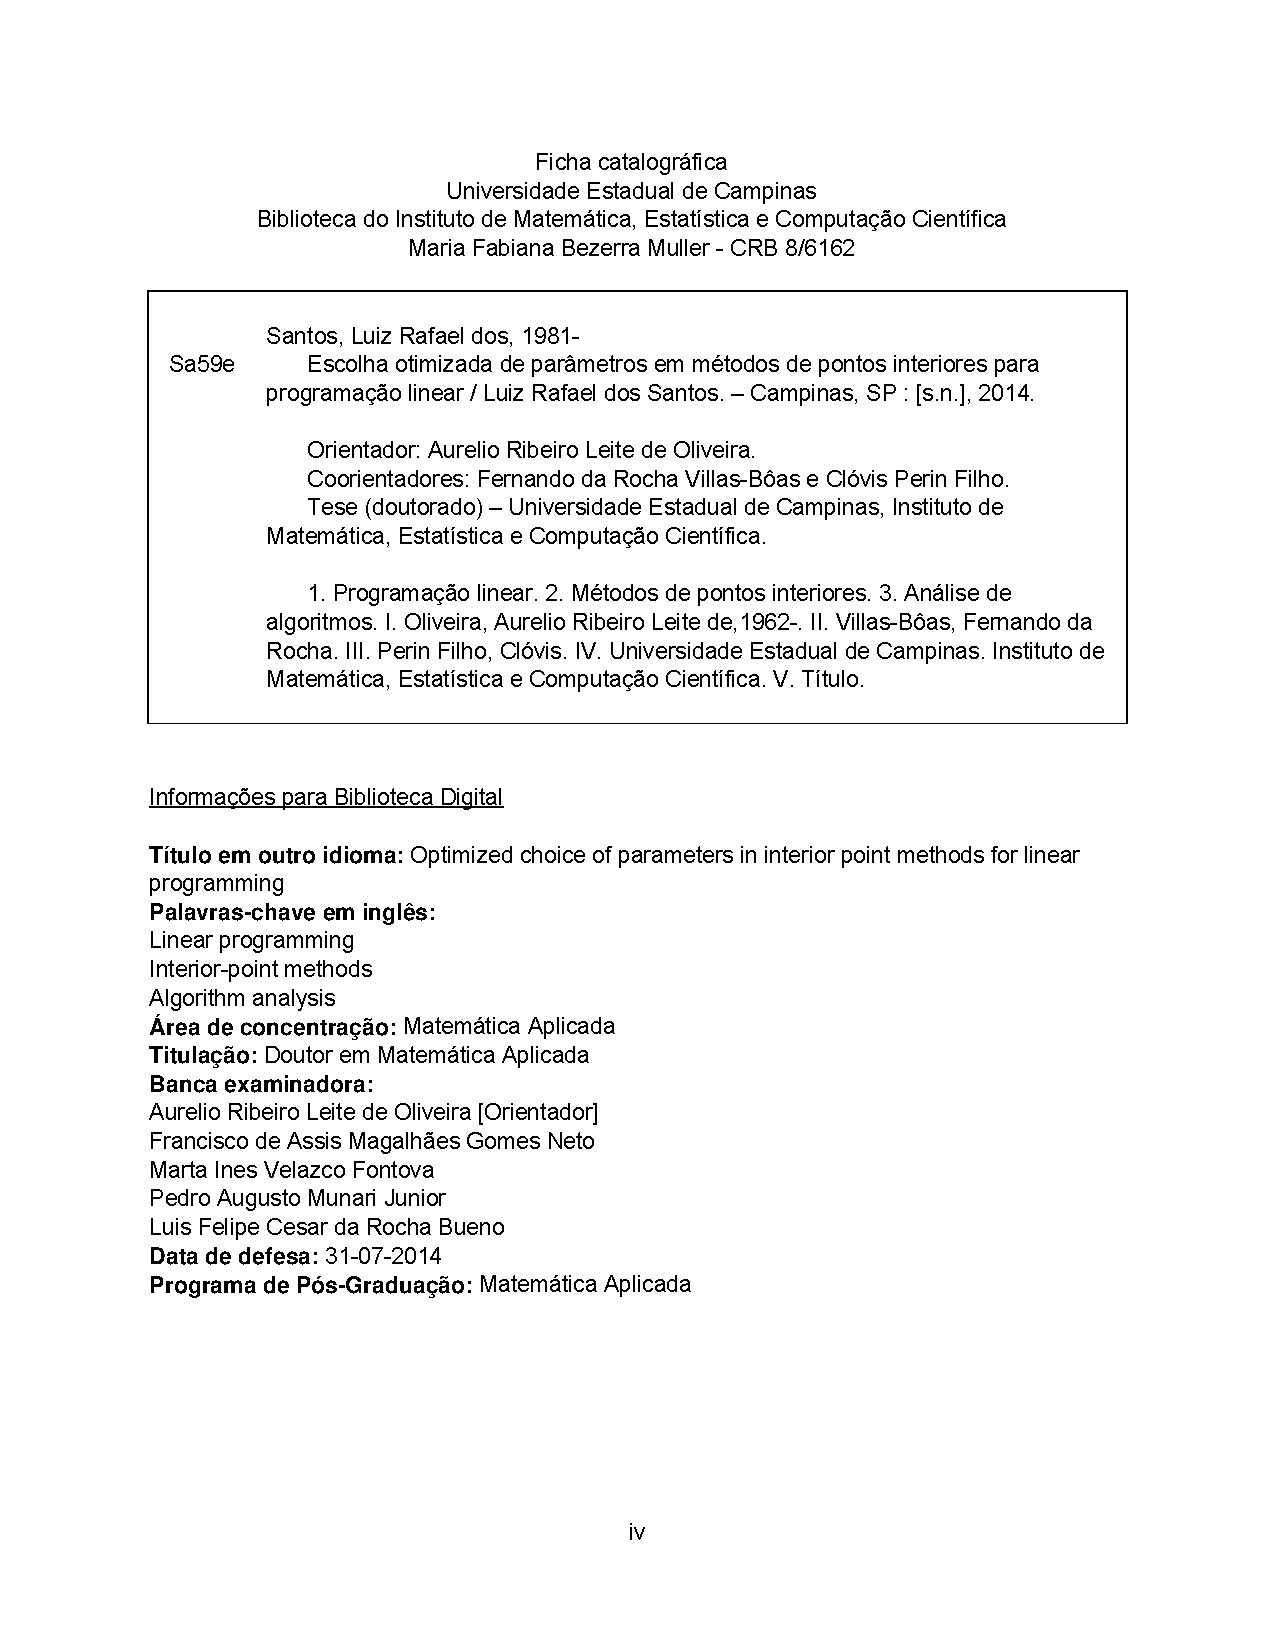
\includepdf{ficha-catalografica}
%
% WARNING A folha de aprovação deve ser assinada pelos membros da banca apos a
% defesa.
% FIXME Substitua o arquivo folha-de-aprovacao.pdf por uma copia escaneada.
 \includepdf[pages=-,pagecommand={\thispagestyle{plain}}]{folha-de-aprovacao1}


\cleardoublepage  % Capítulo vazio.
\begin{center}
  \large{\textbf{Abstract}}
\end{center}

\selectlanguage{english}
% FIXME Delete lines from this one until 14th.



In this work we propose a predictor-corrector interior point method for linear programming in a primal-dual context, in which the next iterate will be chosen by the minimization of a polynomial merit function  of three variables-parameters: the first one is the step length, the second one defines the central path and the last one models the weight that a corrector direction should have. The merit function minimization is performed by subjecting it to constraints defined by a neighborhood of the central path that allows wide steps. In this framework, we combine  different directions, such as predictor, corrector or centering ones, to produce a better direction. Our method generalizes most of predictor-corrector interior point methods, depending on the choice of the variables-parameters described above. Convergence analysis of the method is carried out, by considering an initial point that has good practical performance, which results in Q-linear convergence of the iterates in polynomial complexity. Numerical experiments, using Netlib set test,  showed that this approach is competitive when compared to  well established solvers, such as PCx.




% In this work we solve linear optimization problems on an Interior Point Methods environment by combining different directions, such as predictor, corrector or centering ones, to produce a better direction. We measure how good the new direction is by using a polynomial merit function on three variables. One of them is the step length, the other defines the central path and the last one models the weight that a corrector directions should have in a predictor-corrector method. Some numerical tests show that this approach is competitive when compared to more well established solvers as PCx, using the Netlib test set.

\vspace{.5cm}
\textbf{Keywords}:
% FIXME Remover a linha abaixo.
Linear Programming, Interior Point Methods.
% TODO Inserir as palavras-chave em inglês aqui.
\selectlanguage{brazilian}

\vspace{.05\textheight}
\begin{center}
  \large{\textbf{Resumo}}
\end{center}
\onehalfspacing
Neste trabalho, propomos um método de pontos interiores do tipo preditor-corretor para programação linear em um contexto primal-dual, em que o próximo iterado é escolhido através de um subproblema de minimização de uma função de mérito polinomial a três variáveis: a primeira variável é o tamanho de passo, a segunda define a trajetória central e a última modela o peso que uma direção corretora deve ter.  A minimização da função de mérito é feita  sujeitando-a a restrições  definidas por uma vizinhança da trajetória central que permite passos largos. Dessa maneira, combinamos diferentes direções, tais como preditora, corretora e de centralização, com o objetivo de obter uma direção melhor. O método proposto generaliza grande parte dos métodos de pontos interiores preditores-corretores, a depender da escolha do valor das variáveis  acima descritas. É feita, então, uma análise de convergência do método proposto, considerando um ponto inicial que tem bom desempenho na prática, e que resulta em convergência linear dos iterados em complexidade polinomial. São feitos experimentos numéricos, utilizando o conjunto de testes Netlib, que mostram que essa abordagem é competitiva, quando comparada a implementações de pontos interiores bem estabelecidas como o PCx.


% FIXME Remover deste ponto até a linha 14.
% Esse é o resumo. Ele não deve conter mais de 500 palavras. Uma maneira
% fácil de obter uma boa aproximação do número de palavras do seu resumo é:
% \begin{lstlisting}
% $ detex -l resumo.tex | wc -l
% \end{lstlisting}

% As palavras chaves permitidas podem ser consultadas na
% \href{http://acervus.unicamp.br/}{Base Acervus}, buscando pelo campo
% \emph{Assunto}.
% TODO Inserir o resumo em português aqui.


\textbf{Palavras-chave}:
% FIXME Remover a linha abaixo.
Programação Linear, Métodos de Pontos Interiores, Análise de algoritmos.
% TODO Inserir as palavras-chave aqui.

%
\tableofcontents
%
% FIXME Se não for incluir a dedicatória, comentar a linha abaixo.
  %!TEX root = tese.tex
%======================= DEDICAT\'{O}RIA ==================================

\chapter*{\markboth{}{}}  % \markboth{}{} é utilizado para corrigir o cabeçalho.
\phantomsection
\addcontentsline{toc}{chapter}{Dedicatória}
\begin{center}
  \emph{
  % FIXME Remover as duas linhas abaixo.
  Aos meus \ldots. \\
  Para \ldots.} 
  % TODO Inserir a dedicatória aqui.
\end{center}

%
% FIXME Se não for incluir os agradecimentos, comentar a linha abaixo.
 %!TEX root = tese.tex

\addchap{Agradecimentos}
% FIXME Escrever os agradecimentos.
Aqui deve-se agradecer quem merece agradecimento

Se recebeu bolsa de algum órgão de fomento, não esqueça de agradecê-lo.

%
% FIXME Comentar a linha abaixo se não desejar listar as figuras
% apresentadas.
%\renewcommand{\listfigurename}{Lista de Ilustrações}  % CCPG 228/2013
%\listoffigures
%
% FIXME Comentar a linha abaixo se não desejar listar as tabelas
% apresentadas.
%\listoftables
%
% FIXME Comentar a linha abaixo de não for apresentar as
% abreviações e siglas utilizadas.
%\chapter*{Lista de Abreviaturas e Siglas\markboth{Lista de Abreviaturas e Siglas}{}}  % \markboth{}{} é utilizado para corrigir o cabeçalho.

\begin{description}
  % FIXME Remover as duas abreviações/siglas abaixo e incluir as que serão
  % utilizadas.
  \item[FIXME] Indica que algo deve ser consertado.
  \item[TODO] Indica que algo deve ser feito.
\end{description}

%
% FIXME Comentar a linha abaixo se não for apresentar os
% símbolos utilizados.
\chapter*{Lista de Símbolos\markboth{Lista de Símbolos}{}}  % \markboth{}{} é utilizado para corrigir o cabeçalho.

\begin{description}
    % FIXME Remover os dois símbolos abaixo e incluir as que serão
    % utilizadas.
    \item[$\diamond$] Representa um diamante.
    \item[$\lhd$] Representa um deslocamento para a esquerda.
    \item[$\rhd$] Representa um deslocamento para a direita.
\end{description}

%
% FIXME Comentar a linha abaixo se não desejar listar os algoritmos
% apresentados.
%\listofalgorithms
%
% FIXME Comentar a linha abaixo se não desejar listar os trechos de código
% apresentados.
%\lstlistoflistings
%
% As paginas com o conteúdo da tese são numeradas com algoritmos arábicos.
\mainmatter
%
\doublespacing
% FIXME Remover as 3 linhas abaixo.
%!TEX root = tese.tex
\addchap{Introdução}



\section*{Objetivos e estrutura deste trabalho}




Desde que os  \acrodef{MPI}{Métodos de Pontos Interiores} \acf{MPI} Primais-Duais ficaram famosos nos anos 90 e que o Método Preditor-Corretor de \textcite{Mehrotra:1992wr} surgiu em \citeyear{Mehrotra:1992wr}, muito se teme feito na tentativa de estender e melhorar tal método. Algumas das principais questões atuais em \ac{MPI}, incluem o modo como se pode combinar diferentes direções, seja direção corretora, seja preditora, seja ainda alguma outra direção de  ordem superior, tal que uma melhor direção seja gerada em cada passo.  Como veremos a seguir, uma direção pode ser entendida como a solução do sistema de Newton para as condições KKT do problema de  \ac{PL}. Nesse sentido, as direções utilizadas a cada iteração são encontradas através da solução de um sistema linear com a mesma matriz de coeficientes  -- constante em cada iteração --, porém com vetor do lado direito alterado.


\textcite{Gondzio:1996uw}, por exemplo, combina a ideia inicial preditora-corretora de Mehrotra, porém permitindo múltiplas correções em um mesmo iterando, tentado aumentar o tamanho do passo que pode ser dado, impondo que os iterados estejam o mais perto possível da trajetória central. \textcite{Colombo:2008ia} desenvolvem essa ideia, escolhendo as direções preditora e corretora de forma diferente e permitindo, conforme o caso, quantas correções se deseje. 

Um outro caminho é percorrido por \textcite{Jarre:1999tl} que resolvem, em cada iteração, um subproblema que tenta melhorar os resíduos. Tal subproblema  é em si um problema de PL de dimensão bem  menor em relação ao problema original e cujas variáveis são o peso que cada componente da direção que utiliza deve ter. A solução desse subproblema é feita através do método Simplex. Para tais autores, o subproblema que resolvem pode ser entendido como uma forma de buscar o próximo iterando no subespaço gerado pelas direções que utilizam em seu método.


Nesse mesmo sentido, \textcite{Mehrotra:2005do}, também obtém a direção de busca combinando direções corretoras e preditoras  através de um pequeno subproblema de \ac{PL}. Aqui, as múltiplas  direções corretoras são encontradas fazendo uso de informações geradas a partir de um  subespaço de Krylov apropriado.



Além disso, conforme \textcite{Hung:1996br}, métodos de pontos interiores que são seguidores de caminho  -- veja Seção \ref{sec:path-following-methods} --  geram uma sequência de pontos dentro de uma certa vizinhança da  trajetória central, a qual previne os iterados de prematuramente chegarem muito perto da fronteira da região de factibilidade. Para tanto, é necessário impor condições pré-definidas que façam com que o próximo ponto esteja dentro de uma dessas vizinhanças, garantido  o bom desempenho do método. 




Nesta tese, mostraremos algumas alternativas de respostas para  essas e outras questões correlatas. Assim o objetivo principal desse trabalho é \emph{propor} e \emph{implementar} um Método de Pontos Interiores com pontos infactíves para \ac{PL}, do tipo seguidor de caminho, fazendo  uso de polinômios reais nas variáveis $(\al,\mu,\sig)$, em que $\al$ é o tamanho do passo, $\mu$ é o parâmetro que define a trajetória central, e $\sig$ modela o peso que uma direção corretora deve ter; trata-se portanto de um método preditor-corretor. 

Neste sentido, esses parâmetros são vistos como variáveis, e sua escolha é feita de forma adiada, através da solução de um subproblema que minimiza uma função de mérito \emph{preditiva} que é um polinômio nessas três variáveis e que está sujeita a restrições que impõem que o próximo iterando esteja dentro de uma vizinhança da trajetória central. A função de mérito é preditiva, no sentido que prediz os resíduos lineares e complementares do próximo iterado. Esse é  o que chamamos de Método de Escolha Otimizada de Parâmetros (MEOP).


Uma abordagem similar foi proposta primeiramente por \textcite{VillasBoas:2003tg}, em um contexto auto-dual. Já num contexto primal-dual \textcite{VillasBoas:2012ur,VillasBoas2013:wn}, também fazem uso de uma função de mérito polinomial, porém definem uma trajetória central mais geral, que envolve também os resíduos lineares na sua definição.  Em particular, a abordagem desses autores será utilizada para resolver o subproblema que surgir em nosso método.

Além disso, temos o objetivo de \emph{demonstrar} resultados de convergência do MEOP, utilizando as ferramentas de análise numérica para Métodos Preditores-Corretores do tipo Mehrotra infactíveis, apresentadas principalmente por \textcite{Zhang:2006ic} e trabalhos que são sequências desse e das ideias resumidas em \textcite[cap. 7]{Wright:Primal-dual-interior-point:1997h}. Dentre essas ferramentas, há a necessidade de escolher um ponto inicial adequado para que a convergência do método seja garantida.  

Em geral, conforme alerta \textcite[p. 112]{Wright:Primal-dual-interior-point:1997h}, vários autores utilizam pontos inicias que dependem da norma de uma solução ótima, valor que é desconhecido o que torna a implementação do algoritmo impossível, pelo menos da forma como o algoritmo é descrito.  
 Para contornar tal problema,  estabeleceremos uma Condição que o ponto inicial deve satisfazer a fim de que seja possível demonstrar a convergência e a complexidade  do algoritmo. Tal condição deve levar  em conta o tamanho dos dados do problema a  ser  resolvido e a distância entre o ponto inicial e uma solução ótima.  O ponto inicial será escolhido conforme a heurística de \textcite{Mehrotra:1992wr} e mostraremos que esse ponto satisfaz a Condição proposta, pelo menos para todo conjunto de testes que utilizamos. 



Em relação a experimentos computacionais, o objetivo é implementar o método proposto e testá-lo. Para os testes, utilizaremos o conjunto de testes \Netlib\footnote{Disponível em \url{www.netlib.org/lp/data}.}~\cite{Dongarra:1987jk,Gay:1985ts}. Também objetivamos comparar nosso método com o PCx~\cite{Czyzyk:1999hk}, uma implementação do método preditor-corretor de Mehrotra. 



Com o fim de alcançar  esses objetivos, esta monografia foi organizada com a seguinte estrutura: 

\begin{itemize}

	\item nos Capítulos \ref{chap:linprog} e  \ref{chap:mpis} apresentamos o problema de programação linear, bem como o estado da arte no que diz respeito aos métodos de pontos interiores; 
\item no Capítulo \ref{chap:merit-function} apresentamos o
desenvolvimento de um polinômio real de três variáveis e de grau total 6, como função de mérito  que sirva não só como medida
de factibilidade e otimalidade de um ponto, mas que permita escolher, de forma
otimizada, os parâmetros que determinam uma melhor direção em cada iteração
de um método de pontos interiores primal-dual do tipo seguidor de caminhos; 
\item no Capítulo \ref{chap:convergence} fizemos a análise de convergência e de complexidade do método proposto; 
\item no Capítulo \ref{chap:implementa}  relatamos alguns detalhes de nossa implementação, no que diz respeito  ao ponto inicial, ao critério de parada que utilizamos em nosso algoritmo. Além disso, fazemos uma breve explanação de como se resolve o subproblema de otimização que surge em cada iteração, com base em \cite{VillasBoas2013:wn,VillasBoas:2003tg,VillasBoas:2012ur};

\item No Capítulo  \ref{chap:numerical}  descrevemos o conjunto de testes utilizados e relatamos os resultados  numéricos.


\end{itemize}

 De modo a  concluir esta tese, no último capítulo fizemos considerações finais e encaminhamentos para trabalhos futuros.



\setchapterpreamble[u]{% 
\dictum[George B.~Dantzig]{``Linear programming can be viewed as part of a great
revolutionary development which has given mankind the ability to state general
goals and to lay out a path of detailed decisions to take in order to
 `best' achieve its goals when faced with practical situations of great
complexity.''~\cite{Dantzig:2002td}}
}

\chapter{Programação linear}  
   
\label{chap:linprog}

   Neste capítulo será feita uma breve introdução aos problemas de
\acrodef{PL}{Programação Linear} \ac{PL}, bem como a aspectos preliminares de
alguns métodos desenvolvidos para resolvê-los. 

\acl{PL} é um tópico que tem sido amplamente estudado no escopo da otimização e
que ganhou relevância a partir da década de 1940 com os trabalhos de Dantzig,
Kantorovich, Koopmans e von Neumann. A criação do método simplex por Dantzig 
acelerou o interesse pelo tema, já que se encontrou um meio de resolver tal problema. O texto de Dantzig que serve de epígrafe a este capítulo  serve ao mesmo tempo como um resumo histórico do
desenvolvimento da \ac{PL} e a define de maneira genérica.


A partir da necessidade de tratar matematicamente problemas econômicos
e de planejamento militar nos anos que se seguiram à Segunda Guerra Mundial, ao
mesmo tempo em que os computadores passaram a poder realizar operações
matemáticas com maior velocidade, houve um crescimento espantoso da utilização
da \ac{PL} e, por extensão, da otimização em geral. Para um resumo histórico há
boas fontes
\cite{Schrijver:Theory-of-Linear:1986k,Dantzig:Linear-Programming:1963t}.

Um problema de otimização pode ser descrito em termos de variáveis de decisão,
conjuntos de restrições e uma função objetivo. Resolver um problema de
otimização significa encontrar a ``melhor maneira'' na qual as variáveis
satisfaçam as restrições ao mesmo tempo em que se otimiza -- 
minimiza ou maximiza --  a função objetivo. 
 
Um problema de \emph{\acl{PL}}  é um problema de otimização no qual as
restrições e a função objetivo são lineares. A \ac{PL}\footnote{Usaremos
problema de PL e PL como sinônimos.} surge diretamente em várias aplicações
reais, por exemplo, em problemas de economia, logística, planejamento e controle
da produção, entre outros. Ela aparece ainda em aproximações de problemas mais
complexos ou na solução relaxada de problemas de programação inteira ou mista.


    
Matematicamente, podemos escrever qualquer \ac{PL} na seguinte \emph{forma
padrão}:
\begin{equation} \label{eq:introPL-primal}
	\begin{array}{lc}
\displaystyle \min_{x} & c^Tx \\
\text{sujeito a} &\begin{cases} Ax = b \\
				 x \geq 0	
				 \end{cases}
\end{array}.
\end{equation}
em que $A\in \Real^{m\times n}$ e $c$, $x$ e $b$ têm dimensões compatíveis. A
região $\Pset = \{x\in\Real^n | Ax=b \text{ e } x\geq 0\}$ é conhecida como
região factível do problema e é um poliedro com pelo menos um vértice ou
ponto extremo.

Como uma função linear é convexa, problemas de \ac{PL} tem a particularidade
dada pelo seguinte
teorema~\cite[cap.~3]{Bazaraa:2009uu}:

\begin{teo}[Teorema Fundamental da \acl{PL}] \label{teo:fundamental-pl} Em um
problema de \acl{PL} com região factível $\Pset$, ou o valor ótimo da função objetivo é  ilimitado ou então este valor
será atingido em um ponto extremo de  $\Pset$.
\end{teo}


Um conjunto de restrições lineares define um \emph{poliedro} que constitui
então a \emph{região factível}. De acordo com o
Teorema~\ref{teo:fundamental-pl}, uma forma de encontrar a solução de um
problema de \ac{PL} seria percorrer todos os vértices da região factível
comparando os valores da função objetivo e selecionando o melhor dentre eles.

Essa estratégia, no entanto, é pouco eficiente, haja vista o poliedro ser
resultante de um sistema linear de	$m$ restrições e $n$  variáveis $(m<n)$
podendo ter um número de vértices totalizando
\[ 
\binom{n}{m} = \dfrac{n!}{m!(n-m)!} \geq 
\left(\dfrac{n}{m}\right)^m,
\]
quando o problema está na forma padrão. Por conta disso, um método do tipo
exaustão seria pouco eficiente. Por outro lado, o fato de o número de vértices
ser limitado garante terminação finita para qualquer método que funcione desta
forma. Entretanto, esse número é exponencial,
já que 
\[
\left(\dfrac{n}{m}\right)^m \geq 2^m  \text{ para }   n\geq 2m.
\]
Encontrar um \emph{vértice ótimo} de maneira  eficiente é o
segredo dos bons métodos para resolver problemas de \ac{PL}.

Associado a todo problema \ac{PL}, escrito na forma padrão, existe um outro \ac{PL}, chamado \emph{problema dual} dado por
\begin{equation*}
\begin{array}{lc}
\displaystyle \max & b^Ty \\
\text{sujeito a} &\begin{cases} A^Ty \leq c \\
				 y \text{ livre}	
				 \end{cases}\
\end{array}
\end{equation*}
em que $A$, $b$ e $c$ são os mesmos do problema original, que neste caso, é chamado \emph{problema primal}.
A variável $y\in\Real^{m}$ é chamada variável dual. A fim de que tenhamos restrições de igualdade na definição do problema dual, introduzimos  variáveis de folga duais representadas por $z\in\Real^{n}$, tais que $z\geq 0$, obtendo 
\begin{equation}
\begin{array}{lc}
\displaystyle \max & b^Ty \\
\text{sujeito a} &\begin{cases} A^Ty +z =  c \\
				 z\geq 0, \quad y \text{ livre}	
				 \end{cases}\
\end{array}.
\label{eq:introPL-dual}
\end{equation}


Os problemas primal e dual são comumente chamados par primal-dual e as relações existentes entre estes permitiram a criação ou refinamento de diversos métodos para a solução de \ac{PL}~\cite{Bazaraa:2009uu}. No Capítulo~\ref{chap:mpis} faremos uma explanação mais detalhada sobre esses dois problemas, já estudaremos métodos primais-duais.

\section{Método simplex}


O Método Simplex foi apresentado por
\textcite{Dantzig:Maximization-of-a-linear:1951y} em 1947 e foi desenvolvido ao
mesmo tempo em que houve a percepção do poder da \ac{PL} como ferramenta auxiliar na
tomada de decisões. Seu pioneirismo deve-se à busca da solução do \ac{PL}
caminhando pelos vértices de maneira a utilizar o valor da função objetivo para determinar qual o próximo vértice adjacente deve ser
visitado, fazendo assim uma aplicação do Teorema~\ref{teo:fundamental-pl}.

Mais que isso, dado um método de escolha do próximo vértice, o conjunto de
vértices possíveis decresce em cada iteração,  ainda no caso não degenerado.
Degenerescência (primal) ocorre quando um vértice em $\Real^n$ é definido por
$p>n$ restrições, e um passo de tamanho zero pode ser produzido pelo método. Desta
maneira, o método simplex não sairia do lugar, logo nenhuma melhora na função
objetivo seria alcançada. 


O método simplex se mostrou, e ainda se mostra, robusto e eficiente na solução de grande
quantidade de problemas, e por isso mesmo foi considerado \emph{o método
preferencial} para se resolver \ac{PL}. Entretanto, dado o número exponencial
de  vértices possíveis, havia sempre o receio de que seria necessário esforço
exponencial, isto é, que   todos os vértices da região viável fossem
visitados para que se encontrasse a solução ótima. De fato, \textcite{Klee:1972wi}
foram os primeiros a apresentar uma classe de exemplos patológicos para a qual esse
comportamento  do método simplex apareceu. No exemplo criado por estes
autores, com $n$ variáveis e $2n$ restrições, o método simplex de Dantzig 
precisou passar por todos os $2^n-1$ pontos extremos da região viável antes de
encontrar a solução ótima. 


Apesar disso, nenhum caso com número exponencial de iterações foi encontrado na
vida real, e geralmente apenas uma pequena porcentagem de vértices é
consultada até que se chegue a uma solução ótima. Mais que isso, em geral, o método
simplex mostra comportamento polinomial, sendo linear em relação à $m$ e
sublinear em relação à $n$~\cite[pg.~94]{Fang:1993wu}. Um resumo sobre a
eficiência do método simplex pode ser encontrada no artigo
de~\textcite{Shamir:1987th}.
 

\section{Método elipsoide}

Enquanto na prática o método Simplex continuava como o método mais robusto e
eficiente, a busca por um método que tivesse \emph{complexidade polinomial} no pior
caso foi satisfeita por \textcite{Khachiyan:A-polynomial-algorithm:1979y} através
de seu  \emph{Método Elipsoide}. Antes de continuarmos, vale a penas fazermos uma observação sobre o sentido que daremos a complexidade.

\begin{obs}
Neste trabalho, quando mencionarmos \emph{complexidade}, o faremos no sentido de um limitante para o número de iterações apenas, descartando aqui o esforço gasto para calcular cada iteração.
\end{obs}

O  método elipsoide, ao contrário do método simplex,  não se baseia em caminhar pelos
vértices da região factível mas em diminuir o volume de um elipsoide que
contenha um potencial ponto de solução através de um conjunto de desigualdades
lineares estritas.

Inquestionavelmente, o método elipsoide representou um grande avanço teórico,
significando que a \acl{PL} faz parte dos problemas polinomiais, isto é, que
pode ser resolvido por um algoritmo de complexidade polinomial já que provou-se
que este método tem $\mathcal{O}(n^2(1/\eps))$ iterações, em
que $\eps$ é a precisão desejada para o algoritmo.

Todavia, do ponto de vista prático, o método elipsoide não conseguiu competir com o
método simplex~\cite{Bland:1981vn}, pois sua convergência era muito lenta, na
presença de erros de arredondamento perdia robustez e em cada iteração a
quantidade de memória necessária para armazenamento era muito grande, tornando a iteração cara.
Consequentemente, embora desafortunadamente o método simplex tenha complexidade
exponencial na análise do \emph{pior caso}, experimentos numéricos indicaram que
na prática este era absolutamente superior ao método elipsoide.


\section{Métodos de pontos interiores}



Em problemas práticos, o método Simplex reinou absoluto na solução de problemas
de \ac{PL} até meados da década de 1980 como único método viável para resolver
tal classe de problemas. Em 1984, \textcite{Karmarkar:1984cp} inicia uma nova
abordagem que ficou conhecida como
\acf{MPI} . Por outro lado,  em 1967,
\textcite{DIKIN:InterativeSol1967} já havia publicado um trabalho, no qual um 
 um método de pontos interiores é apresentado. O método de Dikin ficou
conhecido como método afim-escala.
      
% De fato, uma busca histórica mostra que em 1955  o primeiro \emph{\acl{MPI}} é
% atribuído a \textcite{Frisch:The-logarithmic-potential:1955t}.
% Este trabalho implementa uma função barreira-logarítmica para encontrar o mínimo local de uma
% função \emph{não-linear}, sujeita a restrições de desigualdade. O método foi
% extensamente estudado por \textcite{Fiacco:Nonlinear-programming::1968y}, porém
% caiu em desuso por conta de sua ineficiência bem como pela presença de
% competidores muito fortes como a programação quadrática sequencial.



A ideia principal dos \ac{MPI} difere-se fundamentalmente da que inspira o
método simplex. No método simplex as soluções encontradas em cada iteração estão
na fronteira da região factível, já que o método visita os vértices do poliedro
que define tal região. Por outro lado, nos \ac{MPI} estas soluções em cada
iteração estão no interior de uma região. 

Isto é feito criando-se uma família
parametrizada de soluções que convergem assintoticamente para uma solução exata,
isto é, temos de um método homotópico. Com efeito, um \ac{MPI} basicamente utiliza um método do tipo Newton nas condições de otimimalidade de Primeira Ordem, ou Condições KKT, do Problema de Programação Linear. Há, nos diferentes métodos, variação  do lado direito que se usa na solução da linearização das condições KKT que o Método de Newton utiliza, podendo gerar, nesse caso,  direções de Newton diferentes. Daí o nome \emph{Métodos} de Pontos Interiores. 

Em resumo,  uma abordagem não-linear é utilizada para resolver um problema
linear, escapando então da  dificuldade que a dimensão do problema apresenta ao
se lidar com as características combinatoriais  do \ac{PL}.


Além disso,  como exposto acima,  no método simplex a quantidade de
iterações cresce de acordo com o tamanho do problema,  o que não se repete
nos \ac{MPI}. Do ponto de vista
da complexidade computacional, esse método também é polinomial,  com
$\mathcal{O}(n(1/\eps))$ iterações~\cite{Karmarkar:1984cp}.
 
  
Ao contrário do método elipsoide, o método de \citeauthor{Karmarkar:1984cp} tem um desempenho muito
melhor e compete com o simplex, sendo consideravelmente melhor  que este em
problemas de grande porte. Uma variante do método de \citeauthor{Karmarkar:1984cp} foi implementada
por~\textcite{Adler:1989fw}, e desde então a compreensão do funcionamento desses
métodos aumentou consideravelmente, ao mesmo tempo em que variantes têm
sido propostas, muitas delas se apresentando como alternativas computacionais
viáveis ao método simplex.

Atualmente, o melhor algoritmo de pontos interiores conhecido para \ac{PL},  do ponto de vista teórico, 
encontra uma solução com $\eps$-precisão em $\Oset(\sqrt{n}\ln(1/\eps))$
iterações~\cite{Renegar:1988cr}.
De acordo com a teoria geral~\cite[Capítulo 4]{Nesterov:2003wi}, o termo
$\sqrt{n}$  é o melhor que se pode esperar para um \ac{MPI} usando uma função barreira como a
logarítmica. Na prática, no entanto, as implementações de \ac{MPI}  tem desempenho muito melhor que
isso, e em algumas dessas, o número de iterações é quase constante, independente da dimensão do
problema~\cite{Colombo:2008ia}.

Em linhas gerais, há classes de problemas que são melhores resolvidos
pelo método simplex e outras para os quais os métodos de pontos interiores são mais
adequados. Tamanho e estrutura de esparsidade, entre outros, são fatores
preponderantes para a escolha do  método apropriado. Entretanto, pode-se dizer
que com o aumento da dimensão do problema, os \ac{MPI} ficam mais atraentes e
efetivos. Em alguns problemas altamente esparsos e com  estrutura particular é possível uma revisão
do método simplex que o torna muito eficaz~\cite{Hall:2005vw}. Para problemas
de fluxo em rede, nos quais uma especialização do método simplex permite
explorar a estrutura do problema de maneira muito
eficiente~\cite{Nemhauser:Integer-and-combinatorial:1988s}, também é comprovada a eficácia do simplex. Vale a pena notar no entanto que, para um problema de fluxo de rede com de milhões de variáveis, 
\textcite{Resende:1993hh} mostraram que um \ac{MPI} foi mais eficiente.



  




\section{Formulação com variáveis canalizadas e extensões}

Embora a formulação padrão do problema primal de \ac{PL} dada em \eqref{eq:introPL-primal} considera apenas que devamos ter $x$ não-negativo, em problemas práticos, nem sempre isso acontece. 

Podemos ter, por exemplo, alguma componente de $x$ -- ou todo o vetor -- irrestrita ou livre. Para resolver esse problema, considere que $x_{i}$ seja livre, para algum $i$. As variáveis $x_{i}^{+},x_{i}^{-}\geq 0$ são criadas, tais que $x_{i} = x_{i}^{+} -  x_{i}^{-}$. Nesse caso, sessa variáveis substituídas são as restrições do problema e  uma variável livre é trocada por duas variáveis não-negativas. 

Pode haver também algum $x_{i}$ com limitante inferior não nulo, digamos, $\ell\in\Real$. Isto significa que se está exigindo agora $ x_{i}\geq \ell$. Uma forma de  contornar esse problema é  criar a variável $\xtil_{i} = x_{i} - \ell$ e substituir $x_{i}$ por $\xtil +\ell $ nas restrições do problema. Temos, nesse caso, que $\xtil_{i} \geq 0$.


Um caso não menos comum e bastante importante é o da variável $x$ ser canalizada, isto é, possuir algum limitante superior. Queremos dizer com isso que para algum $i$, existe  $u_i>0$ tal que $0\leq x_{i} \leq u_{i}$. Para esse caso, uma saída possível é a seguinte. 

Suponha que existam $p\leq n$ componentes de $x$ que sejam canalizadas. Definimos então a matriz de posto completo $E\in\Real^{p\times n}$, em que cada coluna e cada linha tem exatamente um elemento não nulo e igual a 1. Aqui, $E$  representa a transformação linear $E:\Real^{n}\To \Real^{p}$ que mapeia $x$ em sua parte canalizada $Ex$. Neste caso teremos $Ex \leq u$, em que $u\in\Real^{p}$ é o vetor das canalizações do problema.


Com isso, o \ac{PL} é escrito como 
\begin{equation*}
	\begin{array}{lc}
\displaystyle \min_{x} & c^Tx \\
\text{sujeito a} &\begin{cases} Ax = b \\
								Ex \leq u	\\				 
				 x \geq 0	
				 \end{cases}
\end{array}.
\end{equation*}
Vamos fazer com a desigualdade desapareça das restrições do problema acima, definindo variáveis de folga primais, dadas pelo vetor $s\in\Real^{p}$, tais que $s\geq 0$ e $Ex +s =  u$. Assim, obtemos o \emph{problema primal canalizado}
\begin{equation}
\label{eq:introPL-primal-bounded}
	\begin{array}{lc}
\displaystyle \min_{x} & c^Tx \\
\text{sujeito a} &\begin{cases} Ax = b \\
								Ex +s =  u	\\				 
				 (x,s) \geq 0	
				 \end{cases}
\end{array}.
\end{equation}

A esse problema, associamos o \emph{problema dual canalizado}
\begin{equation}
\label{eq:introPL-dual-bounded}
\begin{array}{lc}
\displaystyle \max_{(y,v)} & b^Ty + u^{T}v \\
\text{sujeito a} &\begin{cases} A^Ty +z + E^Tv =  c \\
								v + w = 0 \\ 
				 (w,z)\geq 0, \quad y,v \text{ livres}	
				 \end{cases}\
\end{array}.
\end{equation}


É possível escrever tais problemas em uma forma matricial como 
\begin{equation*}
	\begin{array}{lc}
\displaystyle \min_{x} & c^Tx \\
\text{sujeito a} &\begin{cases} \bbm A & 0 \\ E & I_{p}\ebm \bbm x\\ s\ebm = \bbm b\\ u\ebm \\			 
				 (x, s) \geq 0	
				 \end{cases}
\end{array}
\quad \text{e} \quad \begin{array}{lc}
\displaystyle \max_{y,v} & b^Ty + u^{T}v \\
\text{sujeito a} &\begin{cases}  \bbm A^{T} & E^{T} \\ 0 & I_{p}\ebm \bbm y\\ v\ebm +\bbm z\\ w\ebm   = \bbm c\\ 0\ebm \\ 
				 (w,z)\geq 0, \quad y,v \text{ livre}	
				 \end{cases}
\end{array}.
\end{equation*}


Sejam $\Atil = \bbm A & 0 \\ E & I_{p}\ebm$,  $\btil = \bbm b\\ u\ebm$, $\ctil = \bbm c\\ 0\ebm$, $\xtil = \bbm x\\ s\ebm$, $\ytil = \bbm y\\ v\ebm$ e $\ztil = \bbm z\\ w\ebm$. Essas definições transformam \eqref{eq:introPL-primal-bounded} e \eqref{eq:introPL-dual-bounded} em
\begin{equation} \label{eq:introPL-primal-dual-bounded-tilde}
	\begin{array}{lc}
\displaystyle \min_{x} & \ctil^T\xtil \\
\text{sujeito a} &\begin{cases} \Atil\xtil = \btil \\
				 \xtil \geq 0	
				 \end{cases}
\end{array} \quad \text{e} \quad \begin{array}{lc}
\displaystyle \max & \btil^T\ytil \\
\text{sujeito a} &\begin{cases} \Atil^T\ytil +\ztil =  \ctil \\
				 \ztil\geq 0 \quad\ytil \text{ livre}	
				 \end{cases}
\end{array}.
\end{equation}

Observe que essa notação transforma o par primal-dual canalizado na forma padrão do par primal-dual padrão. Assim, temos uma vantagem que utilizaremos em todo este trabalho. Isso é feito porque, agora é possível tratar apenas do par primal dual na forma padrão sem canalizações, e a notação acima indica que todos os resultados obtidos também serão estendidos para os problemas canalizados. 

Com isso, a partir de agora, consideraremos apenas \ac{PL} na forma dada em \eqref{eq:introPL-primal} e \eqref{eq:introPL-dual} e faremos comentários relativos a canalizações, quando oportunos, em particular quando tratarmos da implementação.


Conforme dissemos, a presente tese trata de \ac{MPI} para problemas de \ac{PL}, no entretanto tais
métodos também podem ser estendidos com o objetivo de resolver problemas não-lineares
de certos tipos, em geral quando a função objetivo é não linear, porém convexa, mas as restrições são lineares e há a exigência da não negatividade das variáveis. 

Em particular, problemas de \acrodef{QP}{Programação Quadrática} \ac{QP} convexa
são usualmente resolvidos com \ac{MPI}, principalmente
quando são de grande porte e é possível especializar o método~\cite{Gondzio:2010bh}. Com efeito, um \ac{QP} convexo pode ser  escrito como
\begin{equation*}
	\begin{array}{lc}
\displaystyle \min_{x} & x^TQx + c^Tx \\
\text{sujeito a} &\begin{cases} Ax = b \\
				 x \geq 0	
				 \end{cases}
\end{array},
\label{eq:QP}
\end{equation*}
em que $Q\in\Real^{n\times n}$ é simétrica semi-definida positiva, $A\in \Real^{m\times
n}$ e $c$, $x$ e $b$ têm dimensão compatível. Com exceção da matriz $Q$, temos a
mesma estrutura de um \ac{PL}.


Neste capítulo fizemos uma breve introdução à \acf{PL}. No próximo capítulo mencionaremos restultados importantes de PL bem como faremos uma revisão dos Métodos de Pontos Interiores  para \ac{PL}.
%!TEX root = tese.tex
\setchapterpreamble[u]{% 
\dictum[Narenda Karmarkar]{``In the simplex method, the
current solution is modified by introducing a nonzero coefficient for one of the
columns in the constraint matrix.
Our method allows the current solution to be modified by introducing several
columns at once''~\cite{Karmarkar:1984cp}}}


\chapter{Métodos de Pontos Interiores Primais-Duais  para \acl{PL}\label{chap:mpis}}


     

Este capítulo tem o objetivo de apresentar os \acl{MPI} primais-duais seguidores
de caminho. A teoria central que versa sobre \ac{MPI} está bem estabelecida e há
ótimos textos sobre o
assunto~\cite{Vanderbei:2008vp,Wright:Primal-dual-interior-point:1997h,Bazaraa:2009uu,Fang:1993wu}.
Recentemente \textcite{Gondzio:2011ta} fez um resumo histórico, no qual resgata as
principais contribuições no tema.  Estas referências servem como texto
introdutório e foi com base nelas e nos trabalhos de 
 \textcite{Colombo:2008wm} e \textcite{Villas-Boas:2000}, que este capítulo foi
 escrito.
    

     

   
\section{Um método de  pontos interiores}
O  problema de \ac{PL} na forma padrão, 
\begin{equation} %(P) \quad
	\begin{array}{lc}
\displaystyle \min_{x} & c^Tx \\
\text{sujeito a} &\begin{cases} Ax = b \\
				 x \geq 0	
				 \end{cases}\
\end{array}
\label{eq:primal}
\end{equation}
é chamado de \emph{problema primal}.

Associado a todo \ac{PL} existe um outro \ac{PL} chamado 
\emph{problema dual}, o qual consiste nos mesmos dados arranjados de maneira
diferente. O dual de \eqref{eq:primal} é
 \begin{equation}%(D) \quad
	\begin{array}{lc}
\displaystyle \max_{(y,z)} & b^Ty \\
\text{sujeito a} &\begin{cases} A^Ty + z = c \\
				 z \geq 0, \:y \text{ livre}	
				 \end{cases}\
\end{array}
\label{eq:dual}
\end{equation}
em que $A\in \Real^{m\times n}$ é uma matriz de posto completo, $c,x,z\in
\Real^n$, $y,b\in\Real^m$ e $m<n$. Chamamos o vetor $y$ de
\emph{variáveis duais}, enquanto que  $z$ é o vetor das \emph{folgas duais}.
Note que, como $A$ tem posto completo, existe uma relação unívoca entre
$z$ e $y$. 

Sejam
\begin{equation}
\label{eq:primal-dual-feas-set}
\Pset = \{x : Ax = b, x\geq 0\} \quad\text{ e } \quad
\Dset = \{ (y, z) : A^Ty + z = b, z\geq 0\}
\end{equation}
 os conjuntos de pontos factíveis primais e duais 
respectivamente. Usando essa notação, o par primal-dual de
(\ref{eq:primal}-\ref{eq:dual}) pode ser reescrito como
\begin{equation}
\label{eq:primal-dual-reescrito}
\min_x\; c^Tx \; \text{ s.a. }\; x\in \Pset \qquad\text{ e } \qquad
\max_{(y, z)}
b^Tx \; \text{ s.a. }\; (y, z) \in \Dset.
\end{equation}


Denomina-se $\Fset = \Pset\times\Dset$ o conjuntos dos pontos primais-duais
factíveis.
 Para fins de notação, pode-se dizer que se  $w = (x, y, z)$ é primal-dual factível, então $w\in\Fset$. Define-se também os conjuntos \[ \Qset =
 \{w\in\Real^{2n+m}:(x,z)\geq 0\} \] e \[ \Qset^+ = \{w\in\Real^{2n+m}:(x,z) >
 0\} \] respectivamente  como os
conjuntos dos pontos de $\Real^{2n+m}$ não-negativos e positivos nas variáveis
$x$ e $z$.



Com isso, 
\begin{equation}
  	\label{eq:F+}
  	\Fset^+ = \Fset \cap \Qset^+
  \end{equation}   o conjunto dos
pontos primais e duais interiores. Como o próprio nome sugere, em Métodos de 
Pontos Interiores dedica-se especialmente a estudar iterados que estejam
contidos em $\Fset^+$, no caso de métodos factíveis, ou iniciando com pontos em $\Qset^{+}$, no caso de métodos infactíveis. Ainda utilizamos as notações $\Pset^{+}$ e $\Dset^{+}$ para indicar os conjuntos primal e dual estritamente factíveis, isto é, respectivamente.


Neste trabalho, o seguinte pressuposto é assumido como verdadeiro:

\begin{pressup}\label{ass:interior-nonempty}
 O conjunto $\Fset^+$ é não-vazio, isto é, existe $(x,y,z)\in\Fset$, tal que $(x,z)\in\Qset^+$.
\end{pressup}




Com efeito,   o Pressuposto \ref{ass:interior-nonempty} tem como
consequência o fato existir  solução para
\eqref{eq:primal} e para \eqref{eq:dual}~\cite[Teorema 3.1]{Guler:1995wf}.
Mais que isso, a partir desse pressuposto, conhecido como \emph{pressuposto do
ponto interior}, concluímos que o conjunto ótimo primal-dual  é
limitado~\cite[Lema 2.2]{Guler:1995tn}.  Caso
esse pressuposto não seja satisfeito, considera-se permitir que o método aceite
iterados infactíveis ou introduz-se perturbações que aumentem o conjunto
$\Fset$.

  


Apresenta-se agora  alguns resultados bem conhecidos sobre a relação entre o par
primal-dual. 

\begin{lema}[Dualidade Fraca]\label{lema:weak-duality}
Seja $(x,y,z)\in\Fset$. Então $c^Tx \geq b^Ty$.
\end{lema}

\begin{proof}
Como $x\in\Pset$ e $(y,z)\in \Dset$ então vale
\[
c^Tx -  b^Ty = c^Tx - x^TA^Ty = x^T(c - A^ty) = x^Tz \geq 0.
\]
\end{proof}  
O significado da Dualidade Fraca é que o valor objetivo primal serve de
limitante superior para o valor objetivo dual e vice-versa. A diferença $c^Tx - 
b^Ty $ é chamada \emph{gap de dualidade}.
Quando em um ponto $(x,y,z)$ factível, o gap de dualidade é zero, isto é, quando 
tanto o valor objetivo primal quanto dual alcançam seus limites, então este ponto  é
solução ótima primal-dual. Este resultado é formalizado no lema a seguir.


 \begin{lema}[Dualidade Forte]\label{lema:strong-duality}
Um ponto $x\in\Pset$ é ótimo se e somente se existe um par $(y,z)\in\Dset$ tal
que $c^Tx = b^Ty$.
\end{lema}

Uma condição necessária e suficiente para que o problema \eqref{eq:primal} tenha uma solução
factível é que $\Pset \neq \varnothing$.  Além disso, se $\Pset \neq \varnothing$
e $\Dset\neq \varnothing$ então ambos \eqref{eq:primal} e \eqref{eq:dual} admitem solução ótima
 $(x^*,y^*,z^*)$ e pelo Lema \ref{lema:strong-duality} o valor da função
 objetivo coincide neste ponto. Por outro lado, se um dos conjuntos $\Pset$ ou
 $\Dset$ forem vazios, então o outro conjunto será ilimitado ou vazio. Nestes
casos, os problemas (\ref{eq:primal}-\ref{eq:dual}) não terão solução.

Podemos agora expressar condições de otimalidade para \eqref{eq:primal} e \eqref{eq:dual}. Tais
condições  ajudarão a reconhecer quando estes problemas  possuem solução
ótima e por isso podem nos ajudar a desenvolver algoritmos ou métodos para
encontrar tais soluções. As condições de 
\acrodef{KKT}{Karush-Kuhn-Tucker}
\ac{KKT}  expressam uma condição de otimalidade de primeira ordem para um \ac{PL}
e podem ser escritas como 
\begin{subnumcases}{\label{eq:KKT}}
Ax=b,\label{eq:KKT-fac-primal}\\ 
A^Ty + z =c, \label{eq:KKT-fac-dual}\\
XZe =0,  \label{eq:KKT-complementar}\\
(x,z)\geq 0. \label{eq:KKT-nao-negativ} 
\end{subnumcases}
em que $X = \diag(x)$, $Z = \diag(z)$ e $e = (1,\ldots,1)^T$.

 As duas primeiras
equações de \eqref{eq:KKT} são conhecidas como \emph{factibilidade ou
viabilidade primal e dual} -- com exceção feita à não-negatividade  --,
respectivamente.
A equação \eqref{eq:KKT-complementar}
significa que $x_iz_i = 0$, para todo $i=1,2,\ldots,n$, e é chamada de \emph{complementaridade}. A última equação é chamada
de \emph{não-negatividade}. Note ainda que se $(x,y,z)\in\Fset$, então ele
satisfaz \eqref{eq:KKT-fac-primal}, \eqref{eq:KKT-fac-dual} e \eqref{eq:KKT-nao-negativ}.
Isso significa que uma solução ótima é caracterizada pela factibilidade primal e
dual e pela complementaridade. Para pontos não ótimos, mas factíveis, a
complementaridade pode nos dar uma medida da \emph{distância} destes pontos para a
otimalidade:
\begin{equation}
\label{eq:gap-complementarity}
x^Tz = c^Tx - b^Ty.
\end{equation}
A valor $x^Tz$ é chamado \emph{gap de complementaridade}. Quando este 
converge para zero, então tem-se uma solução ótima. Além disso, a igualdade
entre o gap de complementaridade e o gap de dualidade mostrado em
\eqref{eq:gap-complementarity} só vale quando o ponto é factível. 


% \begin{obs}
%  Para fins  de
% notação, dados vetores $u$ e $v$ em $\Real^n$,  o vetor $UVe$ poderá
% ser representado usando-se o produto de Hadamard~\cite[p.~455]{Horn:1985tf},
% isto é, $uv$ é o vetor em $\Real^n$, tal que cada componente  $(uv)_i  = u_iv_i$, para $i=1,\ldots,n$.
% Além disso, a substituição $\xi e$ por $\xi$ pode ser feita, quando  $\xi$ for
% um escalar e $e = (1,\ldots,1)$, sempre respeitando e adequando as dimensões.
% \end{obs}




As equações \eqref{eq:KKT} dão uma condição necessária e suficiente para que
$w^* = (x^*,y^*,z^*)$ seja solução de (\ref{eq:primal}-\ref{eq:dual}), isto é, $x^*$ é
solução de \eqref{eq:primal} e $(y^*,z^*)$ é solução de \eqref{eq:dual}. Consequentemente, um
corolário de \ac{KKT} para \ac{PL} é  o Lema \ref{lema:strong-duality}. 


\subsection{Método Afim-escala\label{sec:affine-scalling}}

Os métodos de pontos interiores primais-duais para \ac{PL}  encontram
$w^*$ resolvendo as equações \eqref{eq:KKT}. Note que a única equação não-linear de
\eqref{eq:KKT} é $XZe=0$ e por conta dela é que aplica-se alguma  variante do
método de Newton, modificando a direção de busca e o tamanho de passo de modo que
\eqref{eq:KKT-nao-negativ} seja  satisfeita \emph{estritamente} em toda iteração. 


Podemos reescrever \eqref{eq:KKT} utilizando uma aplicação
$F:\Real^{2n+m}\to \Real^{2n+m}$ da seguinte maneira:
\begin{subequations}
\label{eq:KKT-Newton}
\begin{gather}
F(w) = \bbm Ax - b \\ A^Ty + z - c \\ xz \ebm = 0\label{eq:KKT-Newton-F},\\
(x,z)\geq 0. \label{eq:KKT-Newton-NN}
\end{gather}
\end{subequations}
Todos os \acl{MPI} primais-duais geram iterados $w^k = (x^k, y^k,z^k)$ que satisfazem
\eqref{eq:KKT-Newton-NN} estritamente, isto é, $(x^k, z^k) > 0$. Esta
propriedade dá origem ao termo \emph{ponto interior}. Ao respeitar estes
limites, impede-se iterados tais que $F(w^k)=0$, mas que  não satisfaçam
$(x,z)\geq 0$. Estes tipos de soluções são facilmente encontrados, no entanto
não nos dão informações úteis para a solução de \eqref{eq:primal} e
\eqref{eq:dual}. Alguns métodos primais-duais exigem que $w^k\in\Fset^+$, ou
seja, que o ponto seja estritamente factível. No entanto, atualmente os métodos
mais competitivos trabalham com pontos infactíveis, exigindo somente que o ponto
seja estritamente interior (veja Seção~\ref{sec:infeasible_inicial_point})

O método de Newton aplicado a \eqref{eq:KKT-Newton-F} dá uma aproximação linear
em torno do ponto atual, obtendo uma direção de busca $\Dew = (\Dex, \Dey,
\Dez)$ resolvendo o seguinte sistema linear

\[
\nabla F (w)\Dew = -F(w)
\]
em que 
\[\nabla F = \bbm A & 0 & 0 \\ 
0 & A^T & I \\
Z& 0 & X
\ebm\] 
é a matriz Jacobiana de $F$. 

No caso de problemas de \ac{QP} como dado em
\eqref{eq:QP}, a diferença  estaria justamente na matriz Jacobiana, que
seria  dada por 
\[\nabla F = \bbm A & 0 & 0 \\ 
-Q & A^T & I \\
Z& 0 & X
\ebm.\] 

A direção de Newton é encontrado 
ao resolver
\begin{equation}
\label{eq:KKT-Newton-step}
\bbm A & 0 & 0 \\ 
0 & A^T & I \\
Z& 0 & X
\ebm
\bbm\Delta x \\ \Delta y  \\
\Delta z\ebm
=
\bbm b - Ax \\
 c- A^Ty - z \\
  -xz
\ebm = \bbm r_P \\ r_D \\ r_C\ebm .
\end{equation}
Se o ponto atual é estritamente
factível, então os resíduos $r_P$ e $r_D$ são nulos.  
 
Um passo na direção $\Dew = (\Dex,\Dey,\Dez)$ é chamado \emph{afim-escala}. Normalmente não é
possível caminhar nesta direção com passo completo, isto é, $w + \Dew$
geralmente viola o limite \eqref{eq:KKT-Newton-NN}. Para evitar essa dificuldade
pode ser feita uma busca linear na direção de Newton tal que o novo iterado
será \[ w + \alpha\Dew \] em que $\alpha \in (0,1]$ é o parâmetro da busca
linear. Mesmo assim, geralmente podemos apenas realizar passos pequenos nesta direção
($\alpha \ll 1$) antes de violar a condição $(x,z) > 0$. Consequentemente passos
puramente afim-escala não nos permitem um bom progresso em direção à solução.


 De modo a poder contornar os problemas do método afim-escala, os métodos
 seguidores de caminho sugerem algumas estratégias diferentes do  procedimento padrão de
 Newton:
 \begin{enumerate}[(i)]
\item Enviesar a direção de busca de modo a fazê-la apontar para dentro do
interior do ortante não-negativo $(x,z)\geq 0$, de tal forma que seja possível
mover-se suficientemente  longe da fronteira de tal ortante, antes que algum componente de
$(x,z)$ se torne negativo.
\item Manter os componentes de $(x,z)$  longe do limite do ortante não negativo.
Direções de busca calculadas por meio de pontos próximos a este limite tendem a
ser calculadas com erros de arredondamento relativamente grandes e pouco
progresso pode ser feito por elas.
 \end{enumerate}
 
 
 \subsection{O método de barreira logarítmica}
\label{subsec:barrier-problem}


Uma maneira de fazer  as duas proposições acima valerem é usar  uma
função barreira logarítmica no \ac{PL}. Dado o \ac{PL} na forma padrão \eqref{eq:primal}, é
possível definir um \emph{problema de barreira} correspondente 
\begin{equation}
\begin{array}{cc}
\displaystyle \min_{x} & \displaystyle c^Tx - \tau\sum_{i=1}^n \ln x \\[6mm]
\text{s.a.} & x\in\Pset^{+}
\end{array}\tag{$P_\tau$},
\label{eq:primal-barrier}
\end{equation}
em que $\tau > 0$ é um escalar, normalmente pequeno, que serve de parâmetro para
uma família de problemas $(P_\tau)$, e que é é chamado de
\emph{parâmetro de barreira}.

A presença da barreira logarítmica na função objetivo de \eqref{eq:primal-barrier} força o
iterado a ficar no interior da região factível, já que há uma penalização muito
pesada quando os pontos estão perto do limite. Por outro lado a influência da
função barreira pode ser controlada através do parâmetro $\tau$. O peso na
barreira regula a distância do iterado para o limite, ou seja, quando $\tau \to
0$,  o problema \eqref{eq:primal-barrier} cada vez mais se parece com o problema \eqref{eq:primal}. Esta
estratégia só é possível se $\Pset^0 \neq \varnothing$. Além disso, se $\Pset$
for limitado então tanto \eqref{eq:primal} quanto \eqref{eq:primal-barrier} admitem solução ótima.

Como a função objetivo de \eqref{eq:primal-barrier} é estritamente convexa, o minimizador desta
função, se existir, pode ser completamente caracterizado pelas condições
\ac{KKT}:

\[
\begin{cases}
Ax  =b,\\ 
\tau X^{-1}e + A^Ty =c,\\
(x,z) > 0. 
\end{cases}
\]
Fazendo $Ze=\tau X^{-1}e$, ou equivalentemente $xz = \tau e$, obtemos a
formulação padrão primal-dual das chamadas \emph{condições \ac{KKT} perturbadas}:

\begin{subnumcases}{\label{eq:KKT-perturbed}}
Ax  =b,\label{eq:KKT-fac-primal-perturbed}\\ 
A^Ty + z =c, \label{eq:KKT-fac-dual-perturbed}\\
xz =\tau e,  \label{eq:KKT-complementar-perturbed}\\
(x,z)  >0. \label{eq:KKT-nao-negativ-perturbed} 
\end{subnumcases}

Se as condições \ac{KKT} perturbadas admitem solução para algum $\hat{\tau} >0$,
então admitem solução para qualquer $\tau>0$. O sistema \eqref{eq:KKT-perturbed}
se aproxima mais e mais de \eqref{eq:KKT} quando $\tau\to 0$ e determina uma
única curva suave, contínua e parametrizada pela variável $\tau$, definida por
$\Cset = \{(x(\tau),y(\tau),z(\tau)):
\tau > 0 \}$. Para cada $\tau$ o ponto da curva é completamente caracterizado
como sendo a solução única do sistema \eqref{eq:KKT-perturbed}.
Além disso, quando  $\tau\to 0$, $\Cset$ converge  para uma solução ótima
prima-dual do \ac{PL}. Essa curva é chamada em \ac{MPI} de \emph{trajetória
central}.  Esta trajetória nos guia para uma solução em que os pares $x_iz_i$
são estritamente positivos e decrescem a zero na mesma taxa de
decrescimento de $\tau$. Estudos sobre a trajetória central pode ser encontrados
em \textcite{Bayer:1989av,Bayer:1989ud,Sonnevend:1986ua,Meggido:Pathways-to-the-optimal:1988u}, entre outros. 

Usando o fato de que para algum $\tau>0$ o ponto $(x(\tau),y(\tau),z(\tau))$ é
primal-dual factível, podemos definir o gap de dualidade $g(\tau)$ para \eqref{eq:primal-barrier}
de forma semelhante à Equação \eqref{eq:gap-complementarity} como função do
parâmetro de barreira:

\begin{equation}
\label{eq:gap-duality-mu}
g(\tau) = c^Tx(\tau) - b^Ty(\tau) =
x(\tau)^T(\tau),
\end{equation}
isto é, para cada valor de $\tau$, o gap de dualidade corresponde ao gap de
complementaridade e logo reduzir um significa reduzir o outro. Além disso, como
$XZe - \tau e = 0$ por \eqref{eq:KKT-complementar-perturbed}, então $x_iz_i =
\tau, i=1,\dotsc,n$ e logo
 \begin{equation}
\label{eq:gap-duality-n-mu}
g(\tau) = x(\tau)^Tz(\tau)= \sum_{i=1}^nx_i(\tau)z_i(\tau) = n\tau.
\end{equation}
Isso significa que quando $\tau\to 0$ temos $g(\tau) \to 0$. As equações
\eqref{eq:gap-duality-mu} e \eqref{eq:gap-duality-n-mu} em conjunto com o fato
de que $c^T x (\tau) \geq c^Tx^* = b^T y^* \geq b^Ty(\tau)$, implicam que

 \[ c^Tx(\tau) \xrightarrow{\tau \to 0} c^Tx^* \quad \text{ e } \quad b^Ty(\tau)
 \xrightarrow{\tau \to 0} b^Ty^*.
\] Assim, as funções objetivos do problema perturbado convergem para aqueles
obtidos por uma solução ótima $(x^*,y^*,z^*)$ do problema original. Mais que isso, vale
o seguinte resultado~\cite{Meggido:Pathways-to-the-optimal:1988u}:
 
 
 \begin{teo}\label{teo:xmu-to-xstar}
 Se um problema de \ac{PL} for primal e dual factível e 
 $A$ for de posto completo, então
  \[
 x(\tau) \to x^* \quad \text{ e } \quad 
 (y(\tau),z(\tau))  \to (y^*,z^*),
\]
sempre que   $\tau\to0$.
 \end{teo}
 
 Este teorema significa que, sob algumas condições, a trajetória central
 converge para a solução ótima dos problemas \eqref{eq:primal} e
 \eqref{eq:dual}. Em consequência disto, a trajetória central  pode ser um bom
 guia para encontrar o conjunto ótimo primal-dual. Métodos que se baseiam na
 trajetória central são chamados \acl{MPI}
\emph{seguidores de caminho}.
 


A solução que se encontra por seguir a trajetória central é caracterizada pela
\emph{complementaridade estrita}. Isso é descrito pelo seguinte resultado.
\begin{teo}[Complementaridade estrita]\label{thm:strict_complementarity}
Se \eqref{eq:primal} e \eqref{eq:dual} forem factíveis, então existe um ponto
$x^*\in\Pset$ e um par $(y^*,z^*)\in\Dset$ tais que 
\[
(x^*)^Tz^* = 0 \text{\quad e \quad} x^*_i+ z^*_i >0, \text{ para }i=1,\ldots,n.
\]
\end{teo}

 

Uma solução $(x^*,z^*)$ que satisfaça o teorema acima é chamada estritamente
complementar. Nesses termos pode-se definir o conceito de partição ótima.
Seguindo as ideias de \textcite{Jansen:1997vy}, definimos o suporte do vetor
$v\in\Real^n$ como
\[
\supp(v) = \{i:v_i>0, i=1,\ldots,n\}.
\]
e a partição do conjunto de índices $\{1,\ldots,n\}$ através da definição dos
conjuntos 
\[
\Bset = \supp(x^*) \text{\quad e \quad } \Mset = \supp(z^*).
\]
Do Teorema \ref{thm:strict_complementarity} segue que essa é uma partição bem
definida, no sentido de que as soluções que possuem a propriedade da
complementaridade estrita satisfazem tanto $\Bset\cap \Mset = \varnothing$
quanto $\Bset\cup\Mset = {1,\ldots,n}$. A noção de complementaridade estrita e
de partição ótima são ideias recorrentes em análises de \ac{MPI}.

Um  fato que vale a pena chamar atenção é que nos casos em que o \ac{PL}
tenha múltiplas soluções, um \ac{MPI} para em uma vizinhança do 
centro analítico da face ótima ao invés de em um vértice, como no método
simplex. Isso significa que de certa maneira, através do conceito de partição
ótima,  pode-se interpretar essa situação como sendo a determinação de
todo o conjunto de soluções ótimas. Em contraste a isso, a escolha do vértice ótimo obtido pelo
método simplex é arbitrária e depende de alguns fatores como regras de
pivoteamento. 

Não raramente, ter uma solução básica que identifica um vértice é equivalente a
encontrar uma solução \emph{exata}. Entretanto, deve-se discutir o que significa de
solução ``exata''. Em vários casos, não é necessária uma precisão adicional de
ter-se uma solução em um vértice, ao invés da solução que se encontra no centro
analítico da face ótima.  Do ponto de vista da programação inteira, temos uma
exceção a esse caso, já que as solução inteiras encontram-se nos vértices do
envoltório convexo de pontos inteiros factíveis. A diferença entre ter ou não
uma base ótima ou uma partição ótima é de importante consequência para o uso de
soluções na análise de sensibilidade \cite{Jansen:1997vy,Yildirim:2001gp}


\textcite{Vavasis:1996bw}
discutiram propriedades da trajetória central, demonstrando que a mesma é caracterizada por
$\mathcal{O}(n^2)$ curvas de alto grau e segmentos nos quais a trajetória é
relativamente reta. Mais que isso, em uma vizinhança
suficientemente pequena do ótimo a trajetória central se torna uma linha reta
e com isto, nesta região, o método apresenta a boa propriedade da convergência quadrática que os métodos do tipo
Newton possuem~\cite{Meggido:Pathways-to-the-optimal:1988u}.
 


Considere o limite de \eqref{eq:primal-barrier} quando $\tau\to \infty$ e
consequentemente encontra-se o ponto do qual a trajetória central inicia. Isso
corresponde a encontrar o ponto $\check{x}$ que minimiza a função de barreira,
isto é, 
\[
\check{x} = \arg \min_{x\in\Pset^+}\left\{-\sum_{i=1}^{n}\ln x_i \right\}.
\]
O ponto $\check{x}$ é o \emph{centro analítico} do politopo factível, e foi
primeiramente estudado por \textcite{Sonnevend:1986ua}. Dada a convexidade estrita
da função de barreira, o conceito de centro analítico está bem definido. Como o
centro analítico minimiza o problema de barreira, ele é o ponto que se encontra
mais distante da fronteira do politopo. Entretanto, existe um problema em
definir a trajetória central em termos de centro analítico: a trajetória central
é afetada pela presença de restrições redundantes. Isso acontece porque tem-se
aqui um conceito exclusivamente analítico, o qual não explora considerações
geométricas. Para vencer essa desvantagem, outros tipos de centro -- centro de
gravidade, centro do elipsoide de volume máximo que pode ser inscrito em
$\Pset$, centro volumétrico  -- podem ser definidos, mas usualmente são muito
custosos de se calcular \cite{Gonzaga:1992uj}.


Tal desvantagem da trajetória central foi  apresentada como potencialmente
geradora de consequências extremas por \textcite{Deza:2006hm}, que conseguiram
replicar o comportamento do método simplex no cubo de Klee-Minty num contexto de
pontos interiores. Isso foi conseguido por patologicamente se adicionar um
número exponencial de restrições redundantes e paralelas às faces do cubo, tal que a trajetória
central torna-se altamente destorcida e está presente em vizinhanças
arbitrariamente pequenas de todos os vértices do cubo. 

Menciona-se aqui o fato de que técnicas de pré-processamento são usualmente
implementadas em códigos maduros de modo a remover tanto quanto possível essas
restrições redundantes, mas embora elas sejam implementadas com heurísticas de
sucesso, geralmente não são ótimas.







 
\section{Métodos seguidores de caminho\label{sec:path-following-methods}}



\subsection{Modelo geral para métodos seguidores de caminho}
 A maioria dos métodos primais-duais seguidores de caminho realizam passos de Newton
 em direção a pontos de $\Cset$ para os quais $\tau>0$, ao invés de passos
 puramente Newton para $F$. Como vimos,  o sistema \eqref{eq:KKT} é resolvido
 por fazer os pares complementares se alinhem (veja Equação
 \eqref{eq:KKT-complementar-perturbed}) ao mesmo tempo em que $(x,z) >0$. Como
 estes passos são enviesados em direção ao ortante positivo definido por
 $(x,z)>0$, usualmente é possível tomar passos maiores que um passo de Newton
 para $F$ antes de violar a restrição de positividade. Para descrever esta busca
 enviesada, introduzimos um \emph{parâmetro de centralização} $\eta\in[0,1]$, na
 equação \eqref{eq:KKT-complementar-perturbed}, que faz com que em cada iteração
 $\tau$ decresça monotonicamente.

 
 As equações para  encontrar a direção de busca tornam-se
  \begin{equation}
\label{eq:KKT-Newton-step-mu-tau}
\bbm A & 0 & 0 \\  
0 & A^T & I \\
Z& 0 & X
\ebm
\bbm\Delta x \\ \Delta y  \\
\Delta z\ebm
=
\bbm r_P \\
 r_D \\
 r_C 
  + \eta \tau e
\ebm = 
\bbm r_P \\ r_D \\ r_{\tau}\ebm,
\end{equation} 
 em que  $\Dew = (\Delta x, \Delta y, \Delta z)$ é um passo de Newton apontando para
$(x(\eta\tau),y(\eta\tau),z(\eta\tau))\in\Cset$ e o par $x_iz_i$ é
igual à $\eta\tau$.  Mesmo nesse caso, a direção de busca encontrada $\Dew$ nem
sempre pode ser utilizada e o novo iterado é calculado novamente usando um teste da razão, isto é, escolhendo $\al_k$, tal
que
\begin{equation}
\label{eq:updating-iterate}
 w^{k+1} = w^k+ \al_k \Dew
\end{equation}
e $(x^{k+1}, z^{k+1})>0$. 

\minisec{O parâmetro $\eta$}
 Por um lado, se $\eta=1$ então
\eqref{eq:KKT-Newton-step-mu-tau} define a \emph{direção de centragem} na qual o
passo de Newton é dado em direção à trajetória central. Embora esta direção se
afaste dos limites do ortante não-negativo, ela pouco ou nada reduz o valor de
$\tau$. Entretanto, ao se mover mais perto de $\Cset$  estes passos formam
uma boa base para um progresso substancial na próxima iteração. Isto porque como
a próxima iteração está mais perto da trajetória central, será possível dar um
passo relativamente grande sem que se deixe o ortante não-negativo. Por outro
lado, se $\eta =0$ temos a direção afim-escala pura como em
\eqref{eq:KKT-Newton-step}. A maioria dos métodos usa valores intermediários de
$\eta$ no intervalo aberto $(0,1)$, de modo a tentar alcançar de maneira
eficiente o duplo objetivo de reduzir $\tau$ e melhorar a centralidade. Esta
escolha é dependente do método.



Vamos definir agora uma maneira de escolher $\tau$ utilizando a equação
\eqref{eq:gap-duality-n-mu}. Considere  dado  um ponto estritamente
factível, isto é, $w^0\in \Fset^+$. Então o valor do parâmetro de
barreira  será dado por 
\begin{equation}
\label{eq:tau_k}
\tau_k = \frac{(x^k)^Tz^k}{n}. 
\end{equation}
Olhando por este ângulo, $\tau_k$ representa a média dos valores dos produtos
$x_i^k z_i^k$. Além disso, com o avanço das iterações, o parâmetro de
centralização $\eta$ faz com  que o problema perturbado que estamos resolvendo
\eqref{eq:KKT-Newton-step-mu-tau} se aproxime cada vez mais do problema original \eqref{eq:KKT-Newton}.

 

Com estes conceitos e ideias em  mão, podemos definir um modelo geral para
métodos primais-duais, dado no Pseudo-Código~\ref{alg:modelo-geral}.
\begin{algorithm}
\caption{Modelo geral para um método primal-dual seguidor de caminho.}
\label{alg:modelo-geral}
\begin{algorithmic}[0] 
\Require  $w^0\in\Fset^+$ 
\State $k\gets 0$
	\Repeat
		\State Resolva \eqref{eq:KKT-Newton-step-mu-tau}  para algum $\eta\in(0,1)$.
		\State Encontre $\al_k$, tamanho de passo factível máximo  na direção $\Dew^k$.
		\State Atualize o iterado conforme \eqref{eq:updating-iterate}.
		\State $k\gets k+1$
\Until{O critério de parada ser satisfeito.}
\end{algorithmic}
\end{algorithm}



\subsection{Vizinhanças da Trajetória Central}
\label{subsec:neighbouhoods}

Um método seguidor de caminho segue  a trajetória central $\Cset$ no interior
da região factível em direção a uma solução ótima. No entanto manter um
iterado exatamente sobre $\Cset$ é um objetivo muito difícil, senão impossível.
Isto porque encontrar um ponto que resolve a condição de complementaridade
perturbada \eqref{eq:KKT-complementar-perturbed} para um $\tau$ específico é um
problema tão difícil quanto resolver o próprio \ac{PL}.


Assim, já que computacionalmente é pouco eficiente caminhar ao longo de uma
direção não-linear, um método seguidor de caminho faz com que os iterados
fiquem em torno de $\Cset$. Isto significa restringir os iterados a uma
\emph{vizinhança} da trajetória central e durante o progresso das iterações
segui-la até uma solução do \ac{PL}. Podemos definir vários tipos de
vizinhanças, no entanto sempre excluimos os pontos $(x,z)$ que estão muito perto
do limite do ortante não-negativo. Com isto  direções de busca calculadas de
qualquer ponto desta vizinhança progridem, mesmo que minimamente, em direção ao
conjunto solução e ao mesmo tempo são obtidas de maneira mais fácil.

As duas vizinhanças de $\Cset$ mais comuns são  $\Nset_2(\theta)$, que tem como base a norma-2 e é definida por
\[
\Nset_2(\theta) = \left\{w\in\Fset^0 : \norm{XZe - \tau e}_2 \leq \theta\tau  
\right\},
\]
em que $\theta \in (0,1)$, e a vizinhança 
$\Nset_{-\infty}(\ga)$, baseada na norma-$\infty$, dada por 
\begin{equation}
\label{eq:infty-neig}
\Nset_{-\infty}(\ga) = \left\{w\in\Fset^0 : x_iz_i\geq \ga\tau\text{, para
todo }i =1,\dotsc,n \right\},
\end{equation}
para algum $\ga\in(0,1)$\footnote{Tipicamente são usados os seguintes valores 
para os parâmetros: $\theta = \num{0,5}$ e $\ga = \num{e-3}$~\cite[pg.
9]{Wright:Primal-dual-interior-point:1997h}.}.

A vizinhança $\Nset_2(\theta)$ é mais restrita já que certos pontos de $\Fset^+$
não pertencem à $\Nset_2(\theta)$, não importando quão perto façamos $\theta$ se
aproximar de seu limitante superior 1. Por outro lado, se um ponto pertence à
$\Nset_{-\infty}(\ga)$, então cada par $x_iz_i$ deve ser pelo menos um múltiplo
$\ga$ de seus valores médios $\tau$. Com efeito, se escolhermos $\ga$ perto de
zero, então quase toda região $\Fset$ estará contida em $\Nset_{-\infty}(\ga)$. 

Mantendo todos os iterados dentro de uma dessas duas vizinhanças, métodos
seguidores de caminho reduzem  os produtos $x_iz_i$ a zero mais ou menos na
mesma taxa.


\ac{MPI} seguidores de caminho são  métodos de homotopia
continuada~\cite{Nazareth:1986jg}
similares aos métodos de homotopia para equações não-lineares gerais. Estes
definem uma trajetória que
deve ser seguida para encontrar a solução. Tradicionalmente, métodos de
homotopia mantem-se em uma vizinhança tubular da trajetória, realizando mudanças
incrementais no parâmetro e perseguindo a trajetória homotópica em busca da
solução. Para \ac{MPI} primais-duais, estas vizinhança são cônicas, ao invés de
tubulares, e tendem a ser amplas e relaxadas  para valores grandes da medida de
dualidade $\tau$, porém se tornam mais estreitas quando $\tau\to0$, por conta da
positividade exigida de $(x,z)$.


 Direções de busca que se baseiam na vizinhança $\Nset_2(\theta)$ podem ser
 utilizadas com $\al=1$, e o parâmetro de barreira decresce pouco em cada
 iteração, dando lugar aos chamados \emph{métodos de passo-curto}. Esta
 propriedade impõe e ao mesmo tempo produz os melhores resultados de
 complexidade existentes para \ac{PL}: algoritmos de passo curto tem
 iterações de ordem $\Oset(\sqrt{n}\ln (1/\eps))$. Os métodos de passo curto
 são os mais simples dos \ac{MPI} pois fixam $\al_k\equiv  1$ e $\eta_k \equiv \eta$
 dependente de $\theta$ e foram introduzidos por
 \textcite{Kojima:1989fw} e \textcite{Monteiro:1989go}. Como a redução do
 parâmetro de barreira é muito pequena, estes tipos de métodos são pouco usados
 na prática.
   
 
 Métodos baseados na vizinhança $\Nset_{-\infty}(\ga)$ permitem iterados que
 seguem a trajetória central de maneira mais relaxada  pois obtém-se mais
 liberdade para manobrar e é possível se aproximar da fronteira da região
 factível. De fato, para $\ga$ pequeno quase todo o conjunto $\Fset^0$ está
 contido em $\Nset_{-\infty}(\ga)$. Por outro lado, direções calculadas a partir
 de pontos desta vizinhança têm propriedades mais fracas e o teste da razão é
 necessário para assegurar a positividade de $(x,z)$. Portanto, métodos que
 levam em conta a vizinhança larga são menos conservadores que os métodos de
 passo-curto e podem decrescer o parâmetro de barreira mais rapidamente. São
 chamados de \emph{métodos de passo-longo}  e implementações eficientes de
 \ac{MPI} baseiam-se em alguma variação de métodos de passo-longo.
 
 \subsubsection{Vizinhança Simétrica}
\label{sec:symmetric-neig}  
 A vizinhança $\Nset_{-\infty}(\ga)$, como vimos,  produz uma boa base para
 métodos práticos, pois permite o parâmetro de barreira reduzir rapidamente.
 Mesmo assim, permite que os iterados produzam produtos $x_iz_i$ muito
 diferentes, já que não impõe uma limite superior para a complementaridade.
 
 Essa dificuldade, quando ultrapassada, permite resultados muito melhores na
 prática, já que os pares $x_iz_i$, quando mal escalados, influenciam o mau
 comportamento do método de Newton.
 
 A razão 
\begin{equation}
\label{eq:ratio-complementarity}
\varrho(xz) = \frac{\min_i\{x_iz_i\}}{\max_i\{x_iz_i\}}
\end{equation}
dá uma medida de proporção entre o maior e o menor par de complementaridade.
 Claramente, $\varrho(xz)\in(0,1)$ e quando o iterado é perfeitamente
centrado, este valor é igual a 1. Uma
análise da medida \eqref{eq:ratio-complementarity} pode ser encontrada em
\textcite{Jansen:1jv}.
 

\textcite{Gondzio:1996uw} e posteriormente \textcite{Colombo:2008wm,Colombo:2008ia}
definiram uma vizinhança que tenta fazer com que em cada iteração tenha-se uma
certa \emph{centralidade} dos iterados.  Por centralidade entenda-se a
dispersão dos pares $x_iz_i$. Quando a discrepância nos
valores dos pares complementares é muito grande, e portanto têm-se pouca
centralidade, as direções de busca não são adequadas, não só com valores
pequenos mas também com valores grandes de $x_iz_i$. Com efeito, \textcite[pp.
26]{Colombo:2008wm} propõe que a noção de dispersão dos produtos
complementares não é adequadamente  representada em um ambiente computacional
por nenhuma das  vizinhanças  $\Nset_{-\infty}$.



Com o propósito de corrigir estes problemas foi proposta a \emph{vizinhança
simétrica} $\Nset_s$, na qual os pares complementares não só satisfazem um limite inferior
mas também um limite superior e é definida como
\begin{equation}
\label{eq:symmetric-neig}
\Nset_s(\ga) = \left\{w\in\Fset^0 : \ga\tau \leq x_iz_i \leq
\frac{1}{\ga}\tau, i=1,\dotsc,n \right\},
\end{equation}
em que $\tau = x^Tz/n$ e $\ga\in(0,1)$.

A vizinhança simétrica \eqref{eq:symmetric-neig}  pode ser considerada uma
extensão de $\Nset_{-\infty}$. No entanto, ela não deixa que os
produtos complementares se tornem muito grandes em relação à média. Além disso, $\Nset_s$ promove uma diminuição dos
pares complementares que são muito grandes, permitindo uma melhor centralidade. 


\textcite{Colombo:2008wm}
determinou o valor de $n$ para o qual a vizinhança simétrica impõe um limite
superior mais estreito:
\[
n> \frac{1+\ga}{\ga}.
\]
Para um $\ga=\num{0.1}$, o limite é estreito sempre que $n>11$. 

Além disso, a complexidade do pior caso  para um método de passo-longo factível
que utiliza a vizinhança simétrica $\Nset_s$ é de ordem $\Oset(n\ln(1/\eps))$ de iterações~\cite{Colombo:2008ia}.
Isso significa que  os limites superiores que diferenciam a vizinhança simétrica
de $\Nset_{-\infty}$ não produzem perdas teóricas, ao mesmo tempo em que,
contribuem com  a possibilidade de deixar os iterados mais centrados.
  
  
De fato, \textcite{Zhang:1993gn}, ao provarem a convergência superlinear de um método
primal-dual, utilizam uma vizinhança com parâmetros simétricos para melhorar os
limites da convergência. No entanto, à época imaginavam que um limite superior,
como o dado por $\gamma\tau$,  não teria significância prática, previsão não se
concretizou~\cite{Gondzio:1996uw,Colombo:2008wm,Colombo:2008ia}.

\subsection{Ponto inicial infactível}
\label{sec:infeasible_inicial_point}

Note que até agora, estamos assumindo que o método inicia  um ponto estritamente
factível $w^0 \in \Fset^0$. Neste caso, $r_P = r_D = 0$, no lado
direito de \eqref{eq:KKT-Newton-step-mu-tau}, e assim a direção de busca
encontrada através desta equação garante que
\begin{equation}
\label{eq:fact-direction}
A\Dex = 0 \quad \text{ e } \quad A^T\Dey + \Dez = 0.
\end{equation}
Consequentemente a factibilidade de todos os iterados é garantida, pois para
$\al =1$ valem as seguintes igualdades:
\begin{gather*}
A(x + \Dex) = Ax + A\Dex = b, \\
A^T(y+\Dey) + (z + \Dez) = (A^Ty + z) + (A^T\Dey + \Dez) = c, \text{ e }\\
\Dex^T \Dez  = - \Dex^T (A^T\Dey) = - (A\Dex)^T\Dey = 0.
\end{gather*}
Métodos que assumem esta hipótese são os chamados \emph{\ac{MPI} factíveis}. 

Ao avaliar o gap de complementaridade quando tomando um passo de
tamanho $\al$ na direção $(\Dex, \Dey, \Dez) $ obtemos
\[
x(\al)^Tz(\al) = x^Tz + \al\left(z^T\Dex +  x^T\Dez + \al^2\Dex^T \Dez  
\right) = \left(1 - \al(1 - \eta) \right)x^Tz,
\]
em que usamos o fato de que $\Dex^T \Dez = 0$, $x^Tz = n\tau$ e que $z^T\Dex
+ x^T\Dez = - x^Tz + n\tau\eta $. Assim, dividindo por $n$ obtemos 
\begin{equation}
\label{eq:progress-opt-feasible}
\tau(\al) = x(\al)^Tz(\al)/n = (1 - \al(1-\eta))\tau.
\end{equation}

A equação \eqref{eq:progress-opt-feasible} mostra que  o progresso na
otimização depende dos parâmetros $\tau$ e $\eta$ bem como do tamanho do passo
$\al$. Este fato motiva a escolha adequada destes valores de modo a obter um
iterado que progrida em direção ao ótimo de maneira mais rápida. 




Nem sempre, porém,  obter um ponto inicial factível é uma tarefa trivial.
É possível, por exemplo, encontrar um ponto inicial factível reformulando o
problema  ou utilizando um método do tipo \emph{Big M}, mas estas
reformulações podem causar distorções, instabilidades numéricas ou aumento de
colunas densas.  Além disso, a região factível pode ter o interior vazio, o que
torna inválida a teoria apresentada até aqui. Uma abordagem totalmente diferente
é baseada na formulação
auto-dual~\cite{Ye:1994gq}, mas, nesse caso, para tornar o problema sempre
factível, aumenta-se o tamanho do problema, o que de certa forma aumenta o tempo computacional por exigir duas retrosubstituições\footnote{Utilizaremos aqui o termo retrosubstituição pra indicar ambas a substituição progressiva e a retrosubstituição.} -- ou
\emph{backsolves} -- adicionais no cálculo de próximo iterado, devido à
introdução de colunas extra.

\subsubsection{Métodos Infactíveis}
Uma alternativa que  permite que essas dificuldades sejam contornadas é utilizar
\emph{\ac{MPI} infactíveis}. Métodos implementados que têm importância
prática fazem uso de pontos
infactíveis~\cite{Gondzio:1996uw,Gertz:2003ji,Czyzyk:1999hk}. Em geral, métodos
infactíveis exigem apenas que para o ponto inicial tenha-se $w^0\in\Qset^+$,
isto é, $(x^0,z^0)$ esteja no ortante positivo. Nesse caso  $r_P^0$ e $r_D^0$
são não-nulos.


A direção de busca ainda é feita segundo \eqref{eq:KKT-Newton-step-mu-tau}, e
portanto tem-se um passo de Newton em direção ao ponto
$(x({\eta\tau}),y({\eta\tau}),z({\eta\tau}))\in\Cset$. Pode-se provar
que se fosse possível dar um passo completo  $(\al=1)$,  a
infactibilidade seria eliminada. No entanto, na prática,  o limite da sequência
de iterados é o ponto ótimo e somente quando o ponto atual está em uma
vizinhança apropriada deste ótimo é que se dá um passo completo.

\textcite{Kojima:1993fe}
estabeleceram resultados de convergência para um \ac{MPI} infactível bem como uma regra para o
tamanho do passo que garante a convergência global do método. Isto é obtido ao
utilizar-se uma vizinhança similar à $\Nset_{-\infty}(\ga)$ (veja equação \eqref{eq:infty-neig}), dada por 
\begin{equation}
\label{eq:infeasible-infty-neig}
\Nset_{-\infty}(\ga,\be) = \left\{(x,y,z) \in\Qset^+ :\frac{\norm{(r_P,r_D)}}{\norm{(r^0_P,r^0_D)}} \leq
\be\frac{\tau}{\tau_0}, 
x_iz_i\geq \ga\tau,\forall i =1,\dotsc,n \right\}, 
\end{equation}
em que $\ga \in(0,1)$ e $\be\geq 1$ são
parâmetros, $\tau_0$ é dado por \eqref{eq:tau_k} e  $r^0_P$, $r^0_D$ são os
resíduos iniciais primais e duais respectivamente.

 
Embora $\Nset_{-\infty}(\ga,\be)$ não exija a factibilidade em cada iteração,
 existe um limitante superior para a infactibilidade,  que tem como
componente principal a medida de  complementaridade $\tau$.
Assim, ao reduzirmos $\tau$ forçamos os resíduos para zero,  reduzindo
a complementaridade e a infactibilidade na mesma taxa. Com efeito, se
$(x(\al),y(\al),z(\al)) = (x,y,z) + \al\De(x,y,z)$, então 
\[
r_P(\al) = (1-\al)r_P \text{ e } 
r_D(\al) = (1-\al)r_D
\]
mostrando que a infactibilidade se reduz linearmente com $\al$.  Assim, se $\al
= 1$, então os resíduos $r_P$ e $r_D$ tornam-se nulos, portanto a factibilidade é
restaurada e  subsequentemente o método infactível torna-se igual a um método
factível, já que todos os próximos iterados estarão em $\Fset^0$.
\textcite{Kojima:1993fe} provaram a convergência global de um método com passos
infactíveis, enquanto \textcite{Zhang:2006ic} provou  a complexidade  de $\Oset(
n^2 \ln ( 1/\eps ) )$ para um método desse tipo. Para uma uma explanação
completa de métodos infactíveis veja \textcite[cap. 6]{Wright:Primal-dual-interior-point:1997h}. 



 
 

 


\section{Métodos de Pontos Interiores na Prática}

\subsection{Método Preditor-Corretor de Mehrotra}
\label{sec:mehrotra-pc-method}
Do ponto de vista prático, a maioria dos códigos de implementação de \ac{MPI}
baseia-se em alguma variação de um método do tipo  preditor-corretor
 devido a \textcite{Mehrotra:1992wr}. O \acrodef{MPC-M}{Método Preditor Corretor de Mehrotra} \ac{MPC-M} baseia-se no modelo geral
para métodos seguidores de caminho, dado no Pseudo-código
\ref{alg:modelo-geral}, mas altera a busca de direção puramente Newton com
correções que são computacionalmente muito baratas  porém que auxiliam a obter uma
melhor direção. Além disso, um escolha adaptativa do parâmetro de centragem
$\eta$ é feita em cada iteração. Atualmente, nos códigos mais utilizados, tanto
acadêmicos como \texttt{BPMPD}, \texttt{HOPDM}, \texttt{OOPS}, \texttt{OOQP},
\texttt{PCx}, bem como  comerciais tais quais \texttt{Cplex}, \texttt{Mosek} e
\texttt{Xpress}, algumas heurísticas e ideias de otimização também foram
incorporadas, de modo que todos são variantes do \ac{MPC-M}.

Este método usa  aproximações de ordem maior da trajetória central $\Cset$ --
abordagem começada  por \textcite{Meggido:Pathways-to-the-optimal:1988u} e mais
tarde desenvolvidas por
\textcite{Monteiro:1990vn} -- e o uso de pontos infactíveis. Segundo \textcite[pg
194]{Wright:Primal-dual-interior-point:1997h},  a contribuição principal
de Mehrotra foi combinar estas ideias existentes da maneira certa e adicionar
heurísticas engenhosas para escolher o parâmetro de centragem (adaptativamente), o tamanho
do passo e o ponto inicial.

Até aqui o tamanho de passo foi sempre considerado igual tanto para o problema
primal, quanto para o problema dual. No entanto, a quase totalidade das
implementações dos métodos de pontos interiores usa passos diferentes para a variáveis
primais e duais. Esta ideia  tem sido usada em
quase todos os desenvolvimentos práticos de métodos primais-duais e  contribui
para reduzir em até 10\% no número de iterações, tendo como base de testes o
conjunto  \texttt{Netlib}~\cite[pg.
195]{Wright:Primal-dual-interior-point:1997h}.

Como se quer que $(x,z)$ permaneça no ortante positivo, emprega-se uma busca
linear a fim de encontrar os tamanhos de passo primal $\al_P$ e dual $\al_D$  tais que
$x+\al_P\Dex >0$ e $z+\al_D\Dez >0$. Para isso, podemos fazer um teste da
razão, isto é,
\begin{equation}
\label{eq:size-step}
\al_P = \al_0\min \left\{- \frac{x_i}{\Dex_i} : \Dex_i <
0\right\}, \qquad \al_D = \al_0\min \left\{- \frac{z_i}{\Dez_i} : \Dez_i <
0\right\}
\end{equation} 
em que $\al_0$ é um fator que garante positividade estrita e em geral vale
$0,9995$. Além disso, embora use-se sempre  algum tipo de vizinhança, muitas
vezes permite-se que o ponto esteja fora da mesma e por isso, perde-se a
propriedade da convergência global em favor da eficiência computacional. 


O método de Mehrotra gera a sequência de iterados infactíveis
$(x,y,z)$, tais que $(x,z)>0$ e a direção de busca consiste em três componentes:
\begin{enumerate}[(i)]
  \item Uma  direção afim-escala \emph{preditora} que nada mais é que uma direção puramente Newton; 
  
  \item Um termo de centralização,
  cujo tamanho é controlado pela escolha de forma adaptativa do parâmetro $\eta$;
   \item Uma direção  \emph{corretora}  que tenta compensar de alguma forma a não-linearidade perdida na direção de Newton.
\end{enumerate}




Para compreendermos melhor o que essas ideias significam, note que no sistema de
Newton \eqref{eq:KKT-Newton-step-mu-tau}, o lado direito pode ser separado da seguinte forma:
\[
\bbm b-Ax \\ c - A^Ty - z \\ -xz + \eta\tau \ebm = 
 \bbm b-Ax \\ c - A^Ty - z \\ -xz  \ebm +  \bbm 0 \\ 0 \\ 
 \eta\tau \ebm.
 \] 


Assim, a direção preditora $(\dex, \dey, \dez)$ é obtida resolvendo-se o
sistema de Newton com o lado direto dado por
 \begin{equation}
 \label{eq:afinne-scale-step}
 \bbm b-Ax\\ c - A^Ty - z \\ -xz  \ebm =  \bbm r_P\\ r_D \\ r_C  \ebm 
 \end{equation} 
 isto é,  $(\dex, \dey, \dez)$  corresponde a direção afim-escala dada em
\eqref{eq:KKT-Newton-step}. Como visto, essa direção otimiza fortemente em
direção aos pontos para os quais a complementaridade é nula. Entretanto, como o
alvo e $XZe = 0$, essas direções podem ser excessivamente influenciadas por
pontos que têm complementaridade pequena, mas que não são ótimos


%XXX: Distraídas? 


\subsubsection{Direção com correção de Segunda Ordem}

O \ac{MPC-M} explora uma direção corretora de centralidade de modo a
tentar remediar pontos que estão mal centrados. Esta direção caminha para
perto da trajetória central e logo reduz o espalhamento dos produtos
complementares em relação à média, embora não busque otimalidade.

Uma ferramenta importante para isso foi a avaliação dinâmica do parâmetro de
centralização $\eta$. Para começar, queremos medir a eficácia da direção
afim-escala, e por isso definimos $\tau_{\text{af}}$ como sendo a média dos valores
hipotéticos para os pares complementares resultantes de um passo na direção
afim-escala, dado por 
\begin{equation}
\label{eq:tau-affine}
 \tau_{\text{af}} = \frac{g_{\text{af}}}{n} = \frac{(x+\al_P^{\text{af}}\dex)^T
(z+\al_D^{\text{af}}\dez)}{n},
\end{equation}
em que $g_{\text{af}}$ é o gap de complementaridade previsto para a direção afim-escala.
Note que $\tau_{\text{af}}/\tau\in(0,1)$. Se $\tau_{\text{af}}\ll\tau$ então a direção afim-escala é
boa e permite uma significante redução do gap de complementaridade. Por outro
lado, se a razão $\tau_{\text{af}}/\tau$ é próxima de 1, então pouco progresso está sendo
feito na direção  $(\dex, \dey, \dez)$ e um parâmetro $\eta$ perto de 1 é
recomendado. Essa escolha faz com que ocorra uma forte centralização, isto é,
move-se para mais perto de $\Cset$, e logo, na próxima iteração, o método está
melhor posicionado para reduzir o gap de complementaridade.

 \textcite{Mehrotra:1992wr} utiliza a seguinte heurística na escolha do parâmetro
 de centralização foi usada:
\begin{equation}\label{eq:Mehrotra-centralizer-parameter}
\eta = \left(\frac{\tau_{\text{af}}}{\tau}\right)^3.
\end{equation}
Essa escolha sugere um parâmetro de barreira dado por 
\begin{equation}\label{eq:Mehrotra-barrier-parameter}
\tau = \left(\frac{g_{\text{af}}}{x^Tz}\right)^2\tau_{\text{af}} =
\left(\frac{g_{\text{af}}}{x^Tz}\right)^3\frac{x^Tz}{n}.
\end{equation}
Assim, se o passo preditor progride bem, $\eta$ é escolhido pequeno e têm-se
pouca centralização. Caso contrário, $\eta$ é escolhido próximo a $\frac{x^Tz}{n}$ e busca-se
uma forte centralização. Mais geralmente, o parâmetro de
centralização pode ser escolhido como
\[
\eta = \left(\frac{\tau_{\text{af}}}{\tau}\right)^p = \left(\frac{g_{\text{af}}}{x^Tz}\right)^p.
\]

Além disso, \textcite{Mehrotra:1992wr} estudou o efeito de diferentes valores de
$p= 1,2,3,4$ em um subconjunto da de problemas da \texttt{Netlib} e conclui que não havia
 muita diferença para $p$ entre 2 e 4.

Para calcular a direção centralizadora, bastaria resolver o sistema de Newton
com lado direito dado por $(0,0,\eta \tau e)$. No entanto, será mais eficiente
calcular esse termo em conjunto com a direção corretora. 

A direção afim-escala corresponde à aproximação linear da trajetória que liga o
ponto atual ao conjunto ótimo.  Esta linearização produz um erro que pode ser
determinado. De fato, assumindo que daremos um passo completo na direção
afim-escala, temos que o vetor dos pares complementares é  dado por \[
\hat{x}\hat{z} = (x+\dex)(z + \dez) = xz + x\dez + z\dex + \dex
\dez =  \dex\dez \] já que ao usarmos o lado direito
\eqref{eq:afinne-scale-step} para resolver o sistema de Newton, temos que
$x\dez  + z\dex  = -xz$. Isso significa que, quando um passo completo é
dado, os produtos $\hat{x}_i\hat{z}_i$ se transformam em $\dex_i\dez_i $, ao
invés de se anularem como era esperado. Este é exatamente o erro da aproximação linear e
um passo corretor $(\Decox, \Decoy, \Decoz)$ é dado para tentar compensá-lo.

Pode-se ainda ver que, idealmente, deseja-se que o próximo ponto 
satisfaça  \[ (x+\Dex)(z+\Dez) =\eta\tau , \] o que é equivalente a resolver
o sistema não linear \[ z\Dex + x\Dez = -xz + \eta\tau 
 - \Dex\Dez . \] Comparando esta equação com
 \eqref{eq:KKT-Newton-step-mu-tau}, vê-se que na direção afim-escala falta
 exatamente o termo $\Dex\Dez$. Para corrigir isso, o sistema de Newton é
 resolvido com o seguinte lado direito
  \begin{equation}
 \label{eq:corrector-centralizer-step}
 \bbm 0\\ 0 \\ - \dex \dez  + \eta\tau  \ebm, 
 \end{equation}
 encontrando a direção $(\Decox, \Decoy, \Decoz)$. Note que tal direção
 combina a centralização e o termo de segunda ordem   que é o 
 erro da linearização.
 
 Uma vez que as direções preditora e corretora foram calculadas, elas são
 simplesmente adicionadas de maneira a ter a direção desejada:
\begin{equation}
\label{eq:Mehrotra-direction}
 (\Dew, \Dey, \Dez) =  (\dex, \dey, \dez) +  (\Decox, \Decoy,
 \Decoz),
\end{equation}
 e o próximo iterado será dado por
\begin{equation}
\label{eq:Mehrotra-updating}
 (x^{k+1}, y^{k+1},  z^{k+1}) =  (x^{k}, y^{k},  z^{k}) + (\al_P\Dex,\al_D \De
 y, \al_D\Dez),
\end{equation}
 em que $\al_P$ e $\al_D$ são os tamanhos de passo primal e dual dado por
 \eqref{eq:size-step}. 
 
 Resumimos o método preditor-corretor de Mehrotra no Pseudo-Código
 \ref{alg:mehrotra}.
 \begin{algorithm}
\caption{Método preditor-corretor de Mehrotra.}
\label{alg:mehrotra}
\begin{algorithmic}[0] 
\Require $(x^0,y^0,z^0)$ inicial tal que $(x^0,z^0) > 0$ 

	\Repeat
		\State Resolva o sistema de Newton com o lado direito dado por
		\eqref{eq:afinne-scale-step}. 
		 \State Encontre tamanho de passo $\al_P^{\text{af}}$ e $\al_D^{\text{af}}$
		 para a direção afim-escala \State Encontre $\tau$, dado por \eqref{eq:Mehrotra-barrier-parameter} e
		 calcule $\eta$ de acordo com \eqref{eq:Mehrotra-centralizer-parameter}.
		 \State Resolva o sistema de Newton com o lado direito dado por
		  \eqref{eq:corrector-centralizer-step}.
		  \State Encontre tamanhos de passos $\al_P$ e $\al_D$  tais que possa se dar
		  um passo factível na direção  \[(\dex, \dey, \dez) +  (\Decox, \Decoy,
		  \Decoz)\] 
		  \State Atualize o iterado conforme 
		  \eqref{eq:Mehrotra-updating}.
		   \State $k\gets k+1$
\Until{O critério de parada ser satisfeito.}

\end{algorithmic}
\end{algorithm}
 
 
 A principal vantagem do \ac{MPC-M} é que, na prática, ele produz tamanho de
 passos maiores antes de violar as restrições de não-negatividade. Isso normalmente
 significa que se está economizando número de iterações: de fato Mehrotra relata
 que temos economia da ordem de 35\% a 50\% quando comparada com outras
 estratégias~\cite{Mehrotra:1992wr}. Nesse
 caso, o custo é apenas de uma retrosubstituição a mais, já que a matriz do
 sistema de Newton é sempre a mesma. Assim, se o custo da fatoração é elevado,
 economia nos custos computacionais também é alcançada por essa técnica. De 
 fato, o método de Mehrotra é vantajoso em relação a todas as implementações
 para programação linear que usam métodos diretos para calcular as direções de
 Newton~\cite[pg. 40]{Colombo:2008wm}.
 
 
 \subsection{Método das múltiplas correções de centralização}
 
O \acl{MPC-M} é baseado na hipótese de que um passo
completo na direção corretora ocorre, o que raramente é possível. Mais que
isso,  tentar corrigir a complementaridade fazendo todos os seus produtos
iguais ao valor $\tau$ é um objetivo muito forte e algumas vezes pouco eficaz. 
É possível minorar estes problemas através de uma extensão do \ac{MPC-M}
que utiliza mais correções lineares de uma forma inteligente.

O \emph{Método de Múltiplas Correções} deve-se a
\textcite{Gondzio:1996uw} e é uma tentativa de melhorar a centralização do iterado
atual. Esta abordagem busca produzir produtos $x_iz_i$ mais homogêneos e forçar
um aumento do tamanho do passo corrigindo o parâmetro de centralização de
Mehrotra.

Implicitamente \textcite{Gondzio:1996uw} utiliza a Vizinhança Simétrica dada 
em \eqref{eq:symmetric-neig}, de modo a ter produtos perto o suficiente da
trajetória central. Nesta descrição o passo será dado na direção
\[
\Dew = 	\DeMew + \DeMuw
\]
em que $\DeMew$ é a direção de Mehrotra \eqref{eq:Mehrotra-direction}, à qual
uma ou mais correções $\DeMuw$ podem ser aplicadas. Outras escolhas da direção preditora 
$\DeMew$ podem ser
feitas~\cite{Colombo:2008ia}.

Dada a direção preditora-corretora $\DeMew$, seja \[ \tilde{\al_P} =
\min(\al_P+\de, 1) \quad\text{ e }\quad\tilde{\al_D} = \min(\al_D+\de, 1) \]
para algum $\de\in(0,1)$ fixo, entendido como uma quantidade desejável de
aumento do passo. Calcula-se o ponto de tentativa \[
\tilde{x} = x +  \tilde{\al_P} \DeMex,\quad\tilde{z} = z +  \tilde{\al_D}
\DeMez \] e os respectivos produtos complementares $\tilde{t} =
\tilde{x}\tilde{z}\in\Real^n$. Note que por aumentar o tamanho do passo, o
ponto de tentativa é infactível (exterior) mas em compensação é utilizado apenas
para buscar corrigir a centralização,  logo não é necessário preocupar-se
com este fato.

Obviamente os produtos $\tilde{t}$ dificilmente serão iguais a $\tau$ como
desejaríamos. Alguns componentes são bem menores que $\tau$ -- inclusive
podendo ser negativos -- e outros muito maiores. Impondo que
$\tilde{t}\in\Nset_s(\ga)$, colocamos limites superiores e inferiores para cada
par complementar, também verificamos as componentes que não satisfazem a
vizinhança simétrica. 

De fato, o que faremos é  mover produtos pequenos
($\tilde{t}_i\leq \ga\tau$) para o limite inferior $\ga\tau$ e produtos grandes
($\tilde{t}_i\geq \ga^{-1}\tau$) para o limite superior $\ga^{-1}\tau$. Os
produtos que estiverem na vizinhança simétrica já satisfazem estes limites e
portante estão razoavelmente pouco dispersos em relação à média. Na prática
estamos movendo os iterados para dentro de $\Nset_s(\ga)$.


Nesse caso, o termo $\DeMuw$ será encontrado resolvendo o sistema de Newton
com o lado direito dado por
\begin{equation}
\label{eq:multiply-correctors-rhs}
r = \bbm 0\\ 0\\ \xi\ebm
\end{equation}
em que a meta $\xi$ é definida como
\[
\xi_i = 
\begin{cases}
\ga\tau - \tilde{t}_i, & \text{se } \tilde{t}_i\leq \ga\tau,\\
\frac{1}{\ga}\tau -
\tilde{t}_i, & \text{se } \tilde{t}_i\geq \ga^{-1}\tau,\\ 
0, & \text{caso contrário}.
\end{cases}
\]

Ressalte-se que o ponto que estamos buscando não pertence à trajetória central
mas à vizinhança simétrica e que nem todos os produtos complementares sofrem
correção. Assim, a meta dada por \eqref{eq:multiply-correctors-rhs} é
realmente alcançada. 

Dada uma nova direção, poderemos repetir o processo de atualizá-la tantas vezes
quantas forem convenientes. Basta fazer-se $\DeMe  \leftarrow \De$ e procurar
novamente a direção $\DeMu$. No entanto, o número máximo de correções de
centralização permitida depende do problema. Tal número é obtido em
\cite{Gondzio:1996uw} de modo heurístico. Note que a direção corretora
obtida é aceita contanto que o tamanho do passo tenha aumentado  uma fração
desejada.


Em códigos como o \texttt{PCx}~\cite{Czyzyk:1999hk}, o
número máximo de correções é calculado considerando-se o esforço relativo entre o
número de operações necessárias para calcular a decomposição da matriz
resultante do sistema de Newton e o número de operações necessárias para fazer a retrosubstituição. Além disso estima-se a redução do número de iterações. Em
\cite{Gondzio:1996uw}  o custo da fatoração não foi
considerado. 
    

As experiências computacionais apresentadas por \citeauthor{Gondzio:1996uw}, principalmente utilizando seu \emph{solver} \texttt{HOPDM} \cite{Gondzio:1995kv,Gondzio:1996uw},   mostram
que a estratégia das múltiplas correções realmente é efetiva, pois os passos
primais e duais calculados para a direção composta são maiores que aqueles
correspondentes à direção preditora.
Isso resulta em uma redução do número de iterações. O custo de cada
correção neste caso é o mesmo, ao contrário de outros métodos cujo custo aumenta a cada
correção. Praticamente todos os códigos modernos utilizam-se desta estratégia
\cite[Apêndice B]{Wright:Primal-dual-interior-point:1997h}. Uma generalização
desta pode ser encontrada em \cite{Colombo:2008ia}, no qual a direção de
busca é dada por $\Dew = \DeMew + \om\DeMuw$ em que usa-se parâmetro de peso
$\om\in(0,1]$. Este peso é encontrado através de uma busca linear tal que
a solução $\hat{\om}$  maximiza o tamanho de passo $\al$.



\subsection{Ponto Inicial}\label{subsec:initial-point}

Como dissemos, códigos práticos que resolvem \ac{PL} através de \ac{MPI}
utilizam pontos infactíveis, exigindo apenas que $(x,z)>0$. Nada
obstante, encontrar tal ponto seja tarefa mais fácil que encontrar
um ponto inicial factível, obviamente deseja-se que a escolha seja feita de forma a
acelerar a convergência do método. 

A escolha de um iterado inicial com boas
propriedades é crítica e é uma tarefa difícil tanto para métodos factíveis
quanto infactíveis. Pede-se que o ponto possua boas propriedades nas
seguintes características: centralidade do ponto e magnitude das
infactibilidades.

\textcite{Mehrotra:1992wr}
introduziu uma heurística para encontrar um ponto inicial que satisfaça essas hipóteses.
Nesta, resolve-se os seguintes problemas de Quadrados Mínimos
\begin{align*}
&\min\: x^Tx\quad \text{s.a.}\quad Ax = b \\
&\min_{(y,z)}\: z^Tz\quad \text{s.a.}\quad A^Ty + z = c 
\end{align*}
que tentam encontrar um ponto $(\tilde{x},\tilde{y},\tilde{z})$ que satisfaça as restrições primais e
duais. As soluções para estes problemas são dada por 
\[
\tilde{x} = A^T(AA^T)^{-1}b, \quad \tilde{y} = (AA^T)^{-1}Ac\quad \text{ e }
\quad \tilde{z} = c - A^T\tilde{y}.
\]
Tal ponto é então transladado para o ortante positivo e o ponto inicial é
dado por
\begin{equation}
	\label{eq:initial-point-mehrotra}
(x^0,y^0,z^0) = (\tilde{x}+ \vartheta_x e,\tilde{y},\tilde{z}+\vartheta_z e),
\end{equation}
em que $\vartheta_x$ e $\vartheta_ z$ são escalares positivos tais que
$(x^0,z^0)>0$.

Essa estratégia de Mehrotra tem algumas questões a serem consideradas. Ela
depende do escalamento da matriz, é afetada pela presença de restrições
redundantes que porventura tenham escapado do pré-processamento, e não garante
que o ponto inicial seja bem centrado. Mesmo assim, é uma estratégia comum em
códigos de pontos interiores por ser considerada uma heurística muito boa para
determinar o ponto inicial, além de ter custo computacional equivalente ao de
uma iteração de um \ac{MPI}.

\textcite{Gertz:2003ji},	  em seu \emph{solver} \texttt{OOQP}, propõem uma
heurística que se baseia nos mesmos princípios -- que o ponto inicial seja ao mesmo tempo
``bem centrado'' e ``não muito infactível'' -- agora para usar um \ac{MPI} no
contexto de Programação Quadrática. Descreveremos a seguir essa heurística, no
contexto de \ac{PL}. 

Primeiramente calcula-se a \emph{norma dos dados}, que é definida como a raiz
quadrada da magnitude do maior elemento dos dados do problema, isto é, o maior
elemento em valor absoluto entre a matriz $A$ e os vetores $c$ e  $b$.
Após isso, faz-se $x$ e $z$ iguais a essa norma dos dados e $y$ igual a zero e a
partir desse ponto, resolve-se o sistema de Newton \eqref{eq:KKT-Newton-step} e
dá-se  um passo completo na direção afim-escala, encontrando-se o ponto
$(\tilde{x},\tilde{y},\tilde{z})$. Certamente esse procedimento resulta em um
ponto infactível. Procede-se então de forma similar à heurística de Mehrotra,
isto é, translada-se $(\tilde{x},\tilde{y},\tilde{z})$ para o ortante positivo. 
Para tal, calcula-se valor
o máximo da violação dos limites das variáveis, digamos 
\[ \vartheta =
\max_{i\in I_V}\{-x_i,-z_i,0\}, \] em que $I_V$ é o conjunto de índices de $x$ e $z$
que violaram a não-negatividade e translada-se o ponto com o valor \[
\tilde{\vartheta}  = 100 + 2\vartheta, \] tal que o ponto inicial seja interior
o suficiente. Com efeito, o ponto inicial será \[ (x^0,y^0,z^0) = (\tilde{x}+
\tilde{\vartheta} e,\tilde{y},\tilde{z}+\tilde{\vartheta} e).
\]
Note-se que tal ponto, assim como o ponto de Mehrotra, também tem custo
computacional de uma iteração de \ac{MPI}.

 As estratégias expostas acima podem ser compreendidas
como uma tentativa de encontrar um ponto inicial que esteja perto o suficiente
da trajetória central, mas com  produtos complementares $x_iz_i$ 
maiores que uma fração adequada de $\tau$, e que a razão \[
\frac{\norm{(r_P,r_D)}}{\tau}
\] não seja muito grande. 

Aliás, note-se que se está  utilizando a \emph{métrica} dada pela vizinhança
$\Nset_{-\infty}(\ga,\be)$ definida em \eqref{eq:infeasible-infty-neig}. Com isso, essas
heurísticas têm como objetivo impedir que o tamanho do passo $\al$ seja muito
pequeno, ao mesmo tempo que tendem a limitar  o valor de $\norm{(r_P^k
,r_D^k)}/{\tau_k}$. Além disso, ao utilizarmos $\Nset(\ga,\be)$, deseja-se que a
infactibilidade seja levada a zero na mesma taxa que o \emph{gap} de dualidade.
Para uma  análise de várias estratégias de pontos iniciais em
\ac{MPI} veja os trabalhos de \textcite{Gertz:2004cw,DApuzzo:2009ks,Andersen:1996un,Vanderbei:1999wv}.




  
\subsection{Critério de Parada}
\label{subsection:termination-criteria}
Os \ac{MPI}, ao contrário do  Simplex, por exemplo, encontram uma solução apenas
assintoticamente. Por conta do parâmetro de barreira $\tau$, um \ac{MPI} jamais encontra
umaa solução exata do problema de \ac{PL}. Com isso, é necessário um critério de
parada que possa decidir quando o iterado atual está próximo o suficiente 
do conjunto solução. 


Códigos práticos de pontos-interiores,  geralmente geram uma sequência de
pontos  $\{(x^k,y^k,z^k)\}$ para os quais $x^k$ e $z^k$
são ambos estritamente positivos. Nenhum desses iterados pode ser uma solução de
fato do \ac{PL} já que para estes, $x^k_iz^k_i>0$, para $k=0,1,2,\ldots$, o que
viola a condição de complementaridade \eqref{eq:KKT-nao-negativ}. Com efeito, os
iterados convergem para um conjunto de soluções sem de fato alcançá-lo, e para
efeitos práticos um iterado avançado  -- $(x^k,y^k,z^k)$ para $k$ suficientemente
grande --  serve muito bem como uma solução aproximada. Para outras aplicações e
para propósitos teóricos, uma solução ótima $(x^*,y^*,z^*)\in\Fset$ pode ser
necessária. Para tanto, nesses códigos,  há uma fase de
\emph{terminação finita}, a qual toma um iterado interior suficientemente avançado
para um ponto em $\Fset$, encontrando, se for o caso, a base ótima. É
necessário também saber quão avançado o iterado precisa ser, tal que
garanta-se que o número de iterações de ponto-interior não seja muito grande. Veja-se o texto de \textcite[Cap. 7]{Wright:Primal-dual-interior-point:1997h} para uma explanação completa sobre terminação finita em \ac{MPI}.

A maioria das implementações de pontos interiores, por estar trabalhando com
precisão finita, garante apenas um certo grau de exatidão ou tolerância, tanto para a factibilidade quanto para a otimalidade. Grande parte
dos códigos utiliza os seguintes critérios~\cite{Gondzio:1996:CVI,Czyzyk:1999hk}:	


\begin{subequations}
\label{eq:termination-criteria}
\begin{align}
	\dfrac{\norm{Ax - b}}{1 + \norm{x}_{\infty}} \leq \tolL,
	\label{eq:termination-criteria-primal}\\ 
	\dfrac{\norm{A^Ty + z - c}}{1 + \norm{z}_{\infty}} \leq
	\tolL,\label{eq:termination-criteria-dual} \\ 
	\dfrac{\abs{c^Tx - b^T y}}{1 + \abs{b^Ty}}\leq
	\tolG.\label{eq:termination-criteria-gap}
\end{align}
\end{subequations}
Os valores de $\tol_{L}$ e $\tol_{G}$ são em geral potências de 10, e  dependem da precisão desejada. Comumente na literatura escolhe-se $\tolL=\tolG=10^{-8}$.  


Os critérios
\eqref{eq:termination-criteria-primal} e \eqref{eq:termination-criteria-dual}
exigem que os resíduos primais e duais sejam menores ou iguais a uma tolerância.
Assim estaríamos, ainda que assintoticamente, com pontos factíveis. O critério
\eqref{eq:termination-criteria-gap} faz uso do Lema
\ref{lema:strong-duality} (Dualidade Forte para \ac{PL}) e é indicador de
otimalidade. Os denominadores em cada critério são construídos de modo a 
permitirem avaliar relativamente tanto viabilidades primal e dual quanto
otimalidade.
  
Um outro conjunto de critérios muito parecido  com
\eqref{eq:termination-criteria}  é
\begin{subequations}
\label{eq:termination-criteria-pcx}
\begin{align}
	\dfrac{\norm{Ax - b}}{1 + \norm{b}} \leq \tol,
	\label{eq:termination-criteria-pcx-primal}\\
	\dfrac{\norm{A^Ty + z - c}}{1 + \norm{c}} \leq \tol,
	\label{eq:termination-criteria-pcx-dual}\\
	\dfrac{x^{T}z}{1 + \abs{c^Tx}}\leq
	\tol,\label{eq:termination-criteria-pcx-gap}
\end{align}
\end{subequations}
em que $\tol = 10^{-8}$. Note que agora, em contraste com
\eqref{eq:termination-criteria}, os denominadores de 
\eqref{eq:termination-criteria-pcx-primal} e
\eqref{eq:termination-criteria-pcx-dual} são fixos, o que de certa maneira
diminui a quantidade de operações, já que não é mais necessário encontrar a
norma  -- ainda que norma-$\infty$ --  dos vetores $x$ e $z$ em cada
iteração. O valor de $x^{T}z$,  é usado em \eqref{eq:termination-criteria-pcx-gap} ao
 invés do \emph{gap} dual  como em \eqref{eq:termination-criteria-gap}, pois além de para pontos factíveis, \emph{gap} dual e \emph{gap} de complementaridade são iguais -- vide Equação \eqref{eq:gap-complementarity} -- é razoável que se $x^{T}z$ convergir para zero, então o \emph{gap} dual também converge para zero.




Todas estas ideias representam o estado da arte no que diz respeito a \ac{MPI}
para problemas de \ac{PL}. Servirão como estrutura e base para os
desenvolvimentos que faremos neste trabalho.
 
%!TEX root = tese.tex
\setchapterpreamble[u]{% 
\dictum[Alfred North Whitehead]{``Every really new idea looks crazy at
first.''}}






	\chapter{Método de Escolha Otimizada de Parâmetros}
\label{chap:merit-function}


Este capítulo tem o objetivo de apresentar o desenvolvimento de uma função de mérito polinomial,  utilizada em cada passo do método de pontos interiores proposto,  que combina três direções -- a direção afim-escala, a direção de centralização e a direção de correção. Além disso, escrevemos a vizinhança $\Nset_{-\infty}$, ajustada para pontos infactíveis, em termos das mesmas variáveis do polinômio. Isso porque a escolha do peso de cada uma das direções,  na direção final, é feita através da  otimização global da função de mérito sujeita a um conjunto de restrições que garantem que o próximo ponto continuará na vizinhança. Os pesos das direções, são em geral parâmetros escolhidos  \emph{a priori}, nos diversos \ac{MPI}.  Em nosso caso, a escolha será determinada em cada iteração do algoritmo, de maneira otimizada.  Esses procedimentos reunidos produzem o que chamamos de   Método de Escolha Otimizada de Parâmetros (MEOP). Além disso, como veremos a seguir,  nosso método é uma generalização de alguns dos \ac{MPI} encontrados na literatura. 

% \section{Um KKT modificado}


O Algoritmo \ref{alg:optimized-choice-of-parameters} resume o MEOP proposto neste capítulo. A escolha do ponto inicial e do critério de parada, serão descritas no Capítulo \ref{chap:implementa}, enquanto os resultados numéricos obtidos estão no Capítulo \ref{chap:numerical}. 

\begin{algorithm}[ht]
\onehalfspacing
\caption{Método de Escolha Otimizada de Parâmetros.}
\label{alg:optimized-choice-of-parameters} \begin{algorithmic}[1]
\Procedure{ResolveLP}{$A,b,c$}
\State $k \gets 0$
\State $(x^0,y^0,z^0) \gets$ \Call{PontoInicial}{$A,b,c$}.
\Comment{Assegure que  $(x^0,z^0)>0$.}
	\Repeat
		\State Resolva   \eqref{eq:affine-scaling-system} e encontre
		$((\dex)^{k},(\dey)^{k},(\dez)^{k})$.
		\State 	Encontre $((\Dex^\mu)^{k},(\Dey^\mu)^{k},(\Dez^\mu)^{k})$ e
		$((\Dex^\sig)^{k},(\Dey^\sig)^{k},(\Dez^\sig)^{k})$ utilizando
		\eqref{eq:De_C}.
		\State Calcule os coeficientes de  $\nextphi(\al,\mu,\sig)$ usando
			\eqref{eq:varphi-coefficients}
		\State Calcule os coeficienes de $g_{L}(\al,\mu,\sig)$ e $g^{i}_{C}(\al,\mu,\sig)$ utilizando \eqref{eq:g_Ci+G_L-explicit}.
		\State Encontre $(\alk,\muk,\sigk)$ resolvendo o subproblema de
		otimização global 
		\eqref{eq:pop-subproblem}.
		\State Garanta que $\alk \in(0,1)$ tal que $(x^{k+1},z^{k+1})>0$ usando \eqref{eq:ratio-test} e faça
		\[
		\begin{aligned}	
		& x^{k+1} = x^{k} + \alk ((\dex)^{k} + \muk (\Dex^\mu)^{k} +
		\sigk(\Dex^\sig)^{k} )
		\\
		& y^{k+1} = y^{k} + \alk ((\dey)^{k} + \muk (\Dey^\mu)^{k} +
		\sigk (\Dey^\sig)^{k} )
		\\
		& z^{k+1} = z^{k} + \alk ((\dez)^{k} + \muk (\Dez^\mu)^{k} +
		\sigk (\Dez^\sig)^{k} ) \end{aligned}. 
		\]		
		\State $k\gets k+1$
	\Until{O critério de parada ser satisfeito.}
\EndProcedure
\end{algorithmic}
\end{algorithm}

 
O esclarecimento de cada passo do Algoritmo \ref{alg:optimized-choice-of-parameters} será feito a seguir, através da explicitação do MEOP. Primeiramente vamos  construir a função de mérito e suas restrições como polinômios. Para esse fim, são necessárias algumas transformações, as quais explanamos a seguir. 

Considere novamente o par primal-dual  (\ref{eq:primal}-\ref{eq:dual}) na sua forma padrão,
i.e.,  

 \begin{equation*}
	\begin{array}{lc}
\displaystyle \min_{x} & c^Tx \\
\text{sujeito a} &\begin{cases} Ax = b \\
				 x \geq 0	
				 \end{cases}\
\end{array}\tag{$P$}
\end{equation*}
e 
 \begin{equation}
	\begin{array}{lc}
\displaystyle \max_{(y,z)} & b^Ty \\
\text{sujeito a} &\begin{cases} A^Ty + z = c \\
				 z \geq 0, \:y \text{ livre}	
				 \end{cases}\
\end{array}.
\tag{$D$}
\end{equation}

Como visto no Capítulo \ref{chap:mpis}, as condições \ac{KKT}  para este
problema são

\begin{subnumcases}{\label{eq:KKT-choice}}
Ax =b,\label{eq:KKT-fac-primal-choice}\\
A^Ty + z =c, \label{eq:KKT-fac-dual-choice}\\
XZe =0,  \label{eq:KKT-complementar-choice}\\
(x,z) \geq 0. \label{eq:KKT-nao-negativ-choice}
\end{subnumcases}
Com isso, dado qualquer $w = (x,y,z)$, os vetores dos resíduos
de \eqref{eq:KKT-choice}, $r_P, r_D$ e $r_C$, podem ser definidos como
\begin{subequations}
\label{eq:KKT-residuals}
\begin{align} 
r_P & =Ax-b,\label{eq:KKT-residuals-a}\\ 
r_D & =A^Ty + z - c,\label{eq:KKT-residuals-b}\\
r_C  &=XZe. \label{eq:KKT-residuals-c}
\end{align} 
\end{subequations}



Seja 
$(x^0,y^0,z^0)$ um ponto inicial que pertença a $\Qset^+$, isto é, um ponto inicial com as componentes de $x$ e de $z$ positivas. Então
\begin{align*} 
r^0_P & =Ax^0-b,\\ 
r^0_D & =A^Ty^0 + z^0 - c, \\
r^0_C  &=X^0Z^0 e > 0. 
\end{align*}
 


No método proposto, vamos garantir que os resíduos primais e duais iniciais
sejam  não-negativos -- veja Observação \ref{obs:Choice-of-merit-function}.
Escolher um $(x^0,y^0,z^0)$ que gere resíduos iniciais desse tipo pode ser
uma tarefa difícil. Assim, a estratégia adotada é definir  $H_P$ e $H_D$,
matrizes diagonais, tais que cada entrada de suas diagonais seja formada segundo as
seguintes regras:
\begin{subequations}
\label{eq:defining_matrices_H}
\begin{equation}
\label{eq:H_P}
 (H_P)_i = \begin{cases} 1,& \text{se } (r^0_P)_i \geq0\\
-1,& \text{se } (r^0_P)_i <0 \end{cases}, 
\end{equation} para $i=1,\ldots,m$, e \begin{equation}
\label{eq:H_D}
(H_D)_j = \begin{cases} 1,& \text{se } (r^0_D)_j \geq 0\\
-1,& \text{se } (r^0_D)_j <0 \end{cases}, 
\end{equation}
 para $j=1,\ldots,n$.
\end{subequations}



Mais que isso, como  $H_D$ e $H_P$ são matrizes de posto completo, o conjunto
solução de  \eqref{eq:KKT-choice} e do sistema 

\begin{subnumcases}{\label{eq:ScaledKKT}}
H_P(Ax-b) =0,\label{eq:ScaledKKT-fac-primal}\\ 
H_D(A^Ty + z -c) =0, \label{eq:ScaledKKT-fac-dual}\\
XZe =0,  \label{eq:ScaledKKT-complementar}\\
(x,z) \geq 0, \label{eq:ScaledKKT-nao-negativ} 
\end{subnumcases}
é o mesmo. De fato, note que apenas estamos multiplicando cada linha do sistema
\ac{KKT} original por um escalar. Além disso, garantimos que
\[H_P(r^0_P)\geq 0 \text{ e }H_D(r^0_D)\geq
0.\]
Tal era o objetivo principal dessas transformações.

A otimalidade do sistema \eqref{eq:KKT-choice} -- bem como de
\eqref{eq:ScaledKKT}  -- é alcançada quando todos os resíduos forem nulos, ou
melhor dizendo, sempre que esses resíduos forem menores ou iguais a uma  
tolerância pré-estabelecida. Assim propomos um método para resolver o sistema
\ac{KKT} escalado que resolva aproximadamente, em cada iteração, para
$(x,y,z)\in\Qset^+$ e algum $\mu>0$, o sistema

\begin{subnumcases}{\label{eq:Homotopy}}
H_P(Ax-b) = 0, \label{eq:Homotopy-fac-primal}\\ 
H_D(A^Ty + z -c) =0, \label{eq:Homotopy-fac-dual}\\
XZe =\mu e,  \label{eq:Homotopy-complementar}\\
(x,z) > 0. \label{eq:Homotopy-nao-negativ} 
\end{subnumcases}


\begin{obs}[Notação]
De acordo com o contexto, considerando que $k$ é a iteração atual, podemos nos abster de indicar a iteração de um vetor ou variável qualquer $t$, isto é, $t^k = t$. Neste caso,  utilizamos do símbolo circunflexo  \^{} sobre um vetor ou variável $t$ qualquer  em questão para indicar seu valor na iteração $k+1$, isto é, $\hat{t} = t^{k+1}$. 


\end{obs}

\section{Direções de busca}
\subsection{Direção Afim-escala}\label{sec:affine-scaling-directions}
 

Como consequência da Seção \ref{sec:affine-scalling}, a direção afim-escala
$(\dew)^k$ que resolve aproximadamente  o sistema \eqref{eq:KKT-choice}
é encontrada através na solução do sistema não linear
\begin{subnumcases}{\label{eq:affine-scaling-system}}
A(\dex)^k + r_P^k = 0, \label{eq:affine-scaling-system-primal} \\
A^T(\dey)^k +(\dez)^k + r_D^k =  0, \label{eq:affine-scaling-system-dual}\\
Z^k(\dex)^k + X^k(\dez)^k +  r_C^k = 0. \label{eq:affine-scaling-system-compl}
\end{subnumcases}

Deixando de utilizar o índice da iteração, para simplificar, podemos encontrar, por meio  da equação \eqref{eq:affine-scaling-system-compl}, o valor de  $\dez$ como
\begin{equation}
\label{eq:de_z}
\dez = -X^{-1}(Z\dex + r_C).
\end{equation}


Se  esta equação for usada e, além disso, $\dez$ for substituído na equação
\eqref{eq:affine-scaling-system-dual}, obtemos o  sistema
\[
\begin{cases}
A\dex + r_P = 0  \\
A^T\dey -X^{-1}Z\dex -X^{-1}r_C + r_D =  0
\end{cases}.
\]
Este sistema é chamado \emph{Sistema Aumentado} e tem sua forma matricial dada
por
\begin{equation*}
\label{eq:Augmented-system}
\bbm  - D^{-1} & A^T \\
A & 0 
\ebm
\bbm \dex \\ \dey
\ebm = 
\bbm - r_D +X^{-1}r_C  \\  -r_P 
\ebm,
\end{equation*}
em que $D = XZ^{-1}$ é não-singular pois $(x,z)>0$. Mais que isso,
$\dex$ pode ser encontrado como 
\begin{align}
\dex& = -D \left( - r_D +X^{-1}r_C - A^T\dey \right) \notag\\
	 &= D\left(r_D -X^{-1}r_C +A^T\dey \right) \notag\\
	 &= D\left(A^T\dey - t\right), \label{eq:de_x}
\end{align}
em que 
\begin{align*}
t &=  X^{-1}r_C - r_D \\
  &= X^{-1}XZe - A^Ty - z + c \\
  &= z - A^Ty - z + c\\
   &= -(A^Ty - c).
\end{align*}

Usando a fórmula para   $\dex$,  a equação
\eqref{eq:affine-scaling-system-primal} torna-se \[AD\left(A^T\dey - t\right) +
r_P = 0\] e logo
\begin{equation}
\label{eq:de_y}
\dey = B(ADt - r_P),
\end{equation}
em que \begin{equation}
\label{eq:define-B}
B = (ADA^T)^{-1}
\end{equation} e portanto $B^{-1}$ é sempre simétrica definida positiva, já que $A$ tem posto completo.
Consequentemente, para encontrar $\dew$ usamos uma fatoração de 
Cholesky de $B^{-1}$ e uma retrosubstituição.
%XXX Como traduzir o Backsolve?

\subsection{A direção ideal}

O método proposto aqui seguirá a estrutura dos  métodos preditores-corretores
(vide Seção \ref{sec:path-following-methods}). Suponha que, dados o ponto $w =
(x,y,z)$ e um parâmetro  $\mu>0$, seja possível  encontrar $\hat{w}$, solução
do sistema
\begin{equation}
	\label{eq:ideal-system}
\begin{cases} 
A\hat{x} -b = 0 \\
A^T\hat{y} +\hat{z} -c = 0 \\
\hat{X}\hat{Z}e = \mu e
\end{cases},
\end{equation}
através de um único
passo \emph{ideal}
 $\Dew = (\Dex,\Dey,\Dez)$, tal que \[ \hat{w} =
w+\Dew.\]

A estratégia adotada neste trabalho para encontrar esse passo ideal é  escrever
$\Dew = \dew + \Decow$, em que  $\dew$ é a direção afim-escala e $\Decow$ é a direção corretora 
\emph{ideal}.

Procedendo com as substituições, na parte linear de \eqref{eq:ideal-system},
temos
\[ A(x+\Dex) - b = A(x+\dex + \Decox) - b = \underbrace{(Ax - b) + A\dex}_{=0
\text{ por \eqref{eq:affine-scaling-system-primal}}} + A\Decox = A\Decox \] 
e
\begin{align*}
A^T(y+\Dey) + (z+\Dez) - c &= A^T(y+\dey+\Decoy) + (z+\dez+\Decoz) - c \\
						  &= \underbrace{A^Ty + z - c + A^T\dey+ +\dez}_{=0 
						  \text{ por \eqref{eq:affine-scaling-system-dual}}} +
						   A^T\Decoy +\Decoz \\
						  &=  A^T\Decoy +\Decoz.
\end{align*} 

Por outro lado, para a parte da complementaridade de 
\eqref{eq:ideal-system}, temos que
\begin{align*}
\hat{x}\hat{z} &= (x + \Dex)(z+\Dez) = xz + x\Dez + z\Dex + \Dex\Dez \\
                &= \underbrace{xz + x\dez + z\dex}_{=0 \text{ por
                \eqref{eq:affine-scaling-system-compl} }}  + z\Dex^c + x\Dez^c + (\dex + \Dex^c)(\dez + \Dez^c) \\
                &=  x\Dez^c  +z\Dex^c + \Dex^c\Dez^c + \dex\dez 
                + \dex\Dez^c + \dez\Dex^c \\
                &=         x\Dez^c  +z\Dex^c + \Dex\Dez.     
\end{align*}
  
Usando tais simplificações, obtemos o seguinte sistema não linear
\begin{equation}\begin{cases}
A\Dex^c =  0\\
A^T\Dey^c +\Dez^c =  0\\
X\Dez^c + Z\Dex^c + \DeX\Dez = \mu e 
\label{eq:corrector-nonlinear}
\end{cases}.
\end{equation}
O vetor $\DeX\Dez$ corresponde a uma correção de segunda ordem, nos moldes dos
trabalhos de \textcite{Mehrotra:1992wr,Gondzio:1996uw}.



A proposta deste trabalho é utilizar uma  forma de generalização das correções
de ordem superior usadas por esses autores.
Essa generalização será feita supondo que para algum escalar
$\sig$ positivo e limitado a aproximação
\begin{equation}
\label{eq:aproximacao-direcao}
\DeX\Dez \approx \sig \deX\dez
\end{equation} 
seja aceitável. Estamos aqui fazendo um abuso de notação, ao utilizar o símbolo $\approx$. O que queremos dizer é que, estamos usando como hipótese que existe $\sig$ tal que $\norm{\DeX\Dez - \sig \deX\dez}$ seja suficientemente pequena.
%\footnote{Neste caso, a notação $u \approx \sig v$ significa que
%  $u$ é um vetor que pertence ao subespaço gerado por $v$.}

Em particular, note
que se  $\sig = 1$ e $\mu = \tau_{\text{af}}^3/\tau$ -- em que $\tau_{\text{af}}$ é dado
na equação \eqref{eq:tau-affine} e $\tau=x^Tz/n$ -- temos o método de
\textcite{Mehrotra:1992wr}. Por outro lado, para \textcite{Gondzio:1996uw}, $\mu$ é
escolhido como no método de Mehrotra e $\DeX\Dez$ é várias vezes aproximado por
direções que projetem, componente a componente, a complementaridade na
vizinhança $N_s(\ga)$. Caso $\mu=0$ e $\sig=1$, e o ponto inicial for factível, temos o método de \textcite{Monteiro:1990vn}.

 De fato, a escolha do valor $\mu$ e a utilização de
correções de ordem superior definem os diferentes tipos de \ac{MPI} que têm sido
utilizados atualmente~\cite{Wright:Primal-dual-interior-point:1997h}. Isso significa que de certa forma, nosso método generaliza alguns dos mais conhecidos \ac{MPI} existentes.




\subsection{Combinando direções}


%XXX:Escrever sobre o trabalho do Fernando


Alguns autores 
combinam direções de correção utilizando pesos para essas direções.
 \textcite{Colombo:2008ia} generalizam e estendem o trabalho de \textcite{Gondzio:1996uw},
fazendo com que a combinação das múltiplas correções   tenha um peso, que é
escolhido fazendo uma busca linear. Já \textcite{Jarre:1999tl}  propõem um subproblema
linear que é resolvido a cada iteração e cuja solução determina os pesos que as direções de 
correções de ordem superior terão na direção final. 

\textcite{VillasBoas:2003tg}, também no contexto primal-dual, estudam algumas
vantagens de adiar a escolha do parâmetro de barreira e do tamanho do passo.
Estes autores mostram que o próximo iterado pode ser expresso por uma função
quadrática do parâmetro de barreira, bem como constatam que tal parametrização é útil
para garantir tanto a não negatividade do próximo iterado quanto a proximidade destes da
trajetória central. 

Uma das principais contribuições do nosso trabalho, através da extensão das ideias
de \textcite{VillasBoas:2003tg}, é a escolha do valor de $\mu$ -- que aqui faz as
vezes de parâmetro que determina a trajetória central -- e de $\sig$ -- que vai pesar a contribuição da correção --  sendo feita de maneira adiada. Por isso tais parâmetros, bem como o tamanho do passo $\al$, estão sendo
tratados como \emph{variáveis}. Para a escolha desses parâmetros, faremos uso de uma
função de mérito, a qual será construída a seguir.
 
Primeiramente, note que a aproximação dada em  \eqref{eq:aproximacao-direcao}
transforma o sistema não linear \eqref{eq:corrector-nonlinear} no sistema linear
\begin{equation}\begin{cases}
\label{eq:linear-sytem-DeXDeZcorrec}
A\Decox = 0 \\
A^T\Decoy +\Decoz = 0 \\
X\Decoz + Z\Decox  = \mu e - \sig\deX\dez
\end{cases}.
\end{equation}
Expressando tal sistema  na  forma
matricial, temos
\begin{equation}
\label{eq:corrector-linear-matrix}
\bbm A & 0 & 0 \\
0 & A^T & I\\
Z & 0 & X \ebm
\bbm \Decox \\ \Decoy \\ \Decoz
\ebm = 
\bbm 0  \\ 0 \\ \mu e - \sig\deX\dez
\ebm.
\end{equation}
As matrizes do lado esquerdo das equações em
\eqref{eq:affine-scaling-system} e \eqref{eq:corrector-linear-matrix} são as
mesmas. Com isso, podemos resolver  \eqref{eq:corrector-linear-matrix} 
utilizando a mesma fatoração de Cholesky de $B^{-1}$ -- veja a Equação~\eqref{eq:define-B}. 

De fato, o lado direito de  \eqref{eq:corrector-linear-matrix} pode ser
reescrito como
\begin{equation}
\label{eq:corrector-linear-matrix-rhs}
\mu\bbm 0 \\  0 \\ e
\ebm + \sig \bbm 0  \\ 0 \\ - \deX\dez
\ebm.
\end{equation}
Portanto, para $\mu,\sig$ quaisquer -- ainda não escolhidos --, é possível
encontrar a direção corretora $\Decow$ como
\begin{equation}
\label{eq:Corrector-spllited}
\Decow = \mu \Dew^{\mu} + \sig
\Dew^{\sig},
\end{equation} 
resolvendo então dois sistemas lineares similares ao utilizado na direção afim (vide  Seção 
\ref{sec:affine-scaling-directions}). 

Com efeito, encontramos 
$\Dew^\mu$ e $\Dew^\sig$  usando a
mesma abordagem da referida seção, i.e., resolvendo
os sistemas $\nabla F(w)\Dew^\mu = (0,0,e)$ e $\nabla F(w)\Dew^\sig = (0,0,-
\deX\dez)$.


Explicitamente, temos
\begin{equation}
\label{eq:De_C} 
\begin{aligned}
& \Dey^{\mu} = B(ADt^\mu )\\
& \Dex^{\mu} = D(A^T\Dey^{\mu} - t^\mu) \\
& \Dez^{\mu} = -X^{-1}(Z\Dex^{\mu} - e)
\end{aligned} \text{\quad e \quad } \begin{aligned}
& \Dey^{\sig} = B(ADt^\sig)\\
& \Dex^{\sig} = D(A^T\Dey^{\sig} - t^\sig) \\
& \Dez^{\sig} = -X^{-1}(Z\Dex^{\sig} + \deX\dez)
\end{aligned}, 
\end{equation}
em que
\[
t^\mu = - X^{-1}e \text{\quad e \quad} t^\sig = X^{-1}\deX\dez.
\]

Desta forma, o maior esforço computacional por iteração do método proposto consiste
em uma fatoração de Cholesky da matriz $B^{-1}$, seguido de três retrosubstituições.
 
 
Definimos o próximo ponto, para cada uma das variáveis, como sendo \[\hat{w} = w
+ \al(\dew + \Decow),\] 
ou ainda, expandindo para cada variável bem como
separando as direções, na forma
\begin{subequations}
\label{eq:next-iterate}
\begin{align}
& \hat{x} = x + \al(\dex + \mu\Dex^\mu + \sig\Dex^\sig ),  \\
& \hat{y} = y + \al(\dey + \mu\Dey^\mu + \sig\Dey^\sig ), \\
% \intertext{e}
& \hat{z} = z + \al(\dez + \mu\Dez^\mu + \sig\Dez^\sig ).
\end{align} 
\end{subequations}

Até o presente momento, a tripla $(\al, \mu,\sig)$, em que $\al$ é o tamanho do
passo, ainda não foi escolhida. Para de fato realizar o passo indicado acima, a
abordagem proposta neste trabalho é tratar algebricamente $(\al, \mu,\sig)$ como
uma tripla de variáveis reais, utilizar no máximo três retrosubstituições para
escolhê-las e finalmente usar a combinação linear das direções $\dew$,
$\Dew^\mu$ e $\Dew^\sig$, com $\al,\mu$ e $\sig$ determinando
as constantes -- ou pesos --  de tal combinação.




A função de mérito, que será  apresentada em sequência, será formulada a partir
dos resíduos do sistema KKT escalado \eqref{eq:ScaledKKT}. Para tanto, na
próxima Seção será mostrado que é possível prever, a depender de
uma escolha de $(\al, \mu,\sig)$, o próximo resíduo deste sistema.


\section{O próximo resíduo}

\begin{defin} 
\label{def:residual-vector}
Definimos  $\rho$, \emph{vetor de resíduos do sistema} \ac{KKT}  escalado
\eqref{eq:ScaledKKT} para um ponto $(x,y,z)$, como
\begin{equation}
\label{eq:residuals}
\rho(x,y,z) = 
\begin{cases}
\rho_P (x,y,z)= H_P(A{x} -b)  \\
\rho_D(x,y,z)= H_D(A^T{y} +{z} -c) \\
\rho_C(x,y,z)= {X}{Z}e
\end{cases}.
\end{equation}

Além disso, seja  $\rho_L = (\rho_P,\rho_D)^T\in\Real^{m+n}$ o \emph{vetor dos
resíduos da parte linear} do  sistema \ac{KKT} escalado. Definimos o
\emph{vetor dos resíduos na iteração $k$} como $\rho^k$.
Por construção $\rho^0>0$ para $(x^0,y^0,z^0)$.
\end{defin} 



Usando a Definição \ref{def:residual-vector}, dado um ponto  $(x,y,z)$, podemos 
prever o resíduo $\nextrho$, para o próximo ponto $(\nextx,\nexty,\nextz)$, a  depender de uma escolha de 
$(\al,\mu,\sig)$, através do Teorema \ref{thm:next=residual}. 

\begin{teo}
\label{thm:next=residual}
O próximo resíduo para o sistema KKT escalado  \eqref{eq:ScaledKKT} é escrito, em
termos da tripla $(\al,\mu,\sig)$, como 
\begin{equation}
\label{eq:next-residual-all}
\nextrho(\al,\mu,\sig) = \bbm (1-\al)\rho_L \\   (1-\al)\rho_C+ \al\mu e + \al(\al-\sig)L_{0,0} +  
\al^2 \La(\mu,\sig) \ebm
% \begin{cases}
% (\hat{\rho}_L)_\ell  = (1-\al)(\rho_L)_\ell ,  \\
% \text{para } \ell= 1,\ldots,n+m. \\
% (\hat{\rho}_C)_j =  (1-\al)(\rho_C)_j+ \al\mu + \al(\al-\sig)(L_{0,0})_j +  
% \al^2 \La(\mu,\sig)_j,
%  \\
%   \text{para } j = 1,\ldots, n.
% \end{cases}
\end{equation}
em que 
\begin{equation}
\label{eq:Lambda-mu-sigma}
\La(\mu,\sig) =  \mu^2
 L_{2,0} + \mu L_{1,0} + \mu \sig L_{1,1} + \sig^2L_{0,2} + \sig
 L_{0,1},
\end{equation}
e
\begin{equation}
\label{eq:defining-Lij}
\begin{aligned}
	L_{0,0} & = \dex\dez, & L_{1,1}  & = \Dex^\mu\Dez^\sig +
			\Dex^\sig\Dez^\mu, \\	
	L_{1,0} &  = \dex\Dez^\mu +
			\dez\Dex^\mu,  & L_{0,1}  & = \dex\Dez^\sig + \dez\Dex^\sig, \\	
	L_{2,0} &  = \Dex^\mu\Dez^\mu,  & L_{0,2}  & = \Dex^\sig\Dez^\sig .\\	
\end{aligned}
\end{equation}

\end{teo}

O Teorema \ref{thm:next=residual} é consequência direta da aplicação
dos Lemas \ref{lemma:linear-residual} e \ref{lemma:nonlinear-residual}, que
consideram a parte linear e não linear de  $\hat{\rho}$ de forma separada. Esses lemas
e suas demonstrações encontram-se na sequência. %no Apêndice
% \ref{sec:tech-resultas}. 
 
\begin{lema}\label{lemma:linear-residual}
O resíduo da parte linear de  \eqref{eq:ScaledKKT} para o próximo iterado é
escrito como

\[
\hat{\rho}_L(\al,\mu,\sig) = (1-\al)\rho_L.
\]
 
\end{lema}

\begin{proof}
Utilizando \eqref{eq:next-iterate} na equação \eqref{eq:ScaledKKT-fac-primal},  temos
\[
\begin{aligned}
\hat{\rho}_P & = H_P(A\hat{x} -b) = H_P(A(x + \al(\dex +
\Decox )) -b) \\ 
			& = H_P(A(x +  \al\dex) - b) +
 \al H_PA\Decox.
\end{aligned}
\]

Como, de \eqref{eq:affine-scaling-system}, $A\dex = b- Ax$, vale a seguinte igualdade:
\[
\begin{aligned}
H_P(A(x +  \al\dex) - b) & = H_P((1-\al)A\dex) \\
							% & = 	 H_P((\al -1)(b-Ax)) \\
							& =  (1 - \al)\underbrace{H_P(Ax - b)}_{\rho_P} 	\\
							& = (1 - \al)\rho_P.					
\end{aligned}
\]
Por outro lado, pela equação \eqref{eq:corrector-nonlinear}, $A\Dex^c= 0$. Logo
$\hat{\rho}_P = (1-\al)\rho_P$.

A prova para parte dual da factibilidade é similar. Com efeito, de   \eqref{eq:ScaledKKT-fac-dual} e  \eqref{eq:next-iterate}, segue
\begin{align}
\hat{\rho}_D & = H_D(A^T\hat{y} + \hat{z} -c)   \notag \\
			& = H_D\left[ A^T\left(y + \al(\dey + \Decoy)\right) + \left(z + \al(\dez + \Decoz )\right)
			-c\right] \notag\\
 			& = H_D\left[A^Ty  + z -c +  \al(A^T\dey + \dez)\right] +
 			\label{eq:next-rho-dual-a} %\\
 			%& \quad + 
 			H_D\underbrace{\left(A^T\Decoy   + \Decoz\right)}_{=0 \text{ por
 			\eqref{eq:corrector-nonlinear}}}. %\notag 
\end{align}


Como, de \eqref{eq:affine-scaling-system-dual}, $A^T\dey + \dez = c - A^Ty - z$, a equação \eqref{eq:next-rho-dual-a}
torna-se
\[
H_D\left[A^Ty  + z -c +  \al(A^T\dey + \dez)\right]  = (1-\al)H_D 
(A^Ty + z - c)  = (1-\al)\rho_D.
\]

Portanto, $ \hat{\rho}_D = (1-\al)\rho_D$.
\end{proof}
 
 
\begin{lema}\label{lemma:nonlinear-residual}
O resíduo da parte da complementaridade de  \eqref{eq:ScaledKKT}, para o próximo iterado é
escrito como
\begin{equation}
\label{eq:next-residual-complementar}
\hat{\rho}_C = (1-\al)\rho_C + \al\mu e+ \al(\al-\sig)L_{0,0} +
\al^2\La(\mu,\sig).
\end{equation}
em que $\La(\mu,\sig)$ é definida por  \eqref{eq:Lambda-mu-sigma}
 os vetores $L_{i,j}$, $i,j \in \{0,1,2\}$ são definidos por
\eqref{eq:defining-Lij}.
\end{lema}

\begin{proof} 
Para encontrar o resíduo da parte complementar para o próximo iterado,
considere que podemos escrever
 $\hat{\rho}_C  =
\hat{x}\hat{z}$. Então, de \eqref{eq:next-iterate}, 
\begin{align}
\hat{x}\hat{z} & = \left(x + \al(\dex + \Decox) \right)\left( z + \al(\dez + \Decoz
)\right) \notag \\
& = \al^2(\dex+\Decox)(\dez + \Decoz) +  \al\left[  (x\dez+z\dex) +
(x\Decoz + z\Decox)\right] + xz .\label{eq:next-residual-complementar-1}
\end{align}


Note que  $ (x\dez+z\dex) = -xz$ por \eqref{eq:affine-scaling-system}. Além
disso usando a equação \eqref{eq:Corrector-spllited}, claramente  $x\Dez^\mu +
z\Dex^\mu = e$ e $x\Dez^\sig + z\Dex^\sig = - \dex\dez$. Então, de \eqref{eq:corrector-linear-matrix},  $(x\Dez^c +
z\Dex^c) = \mu e - \sig\dex\dez$.
 
Assim, a equação \eqref{eq:next-residual-complementar-1} torna-se
\begin{equation}
\begin{aligned}
\hat{x}\hat{z} & =  \al^2(\dex + \Dex^c)(\dez + \Dez^c) + \al (-xz + \mu   e
- \sig\dex\dez) + xz \notag\\
& = t_{1} + t_{2},
\end{aligned}
\end{equation}
em que 
\begin{subequations}
\begin{equation}	
t_{1} = (1-\al) xz + \al\mu e + 
\al(\al-\sig)\dex\dez    
\label{eq:next-residual-complementar-2a}
\end{equation}
e
\begin{equation}
t_{2}=  \al^2\left(\dex\Dez^c + \dez\Dex^c + \Dex^c\Dez^c\right)
\label{eq:next-residual-complementar-2b}
\end{equation}	
\end{subequations}
são variáveis locais.

Como $\Decow = \mu\Dew^\mu + \sig\Dew^\sig$, então
\begin{align*}
\dex\Dez^c &=  \mu\dex\Dez^\mu + \sig\dex\Dez^\sig,\\
\dez\Dex^c &=  \mu\dez\Dex^\mu + \sig\dez\Dex^\sig,\\
\end{align*}
e
\begin{align*}
\Dex^c\Dez^c& =   (\mu\Dex^\mu + \sig\Dex^\sig) (\mu\Dez^\mu
			+ \sig\Dez^\sig) \\ 
			& = \mu^2\Dex^\mu\Dez^\mu + \mu\sig \left(\Dex^\mu\Dez^\sig +
			\Dex^\sig\Dez^\mu \right) + \sig^2\Dex^\sig\Dez^\sig.
\end{align*}
Consequentemente $t_{2}$, dado em \eqref{eq:next-residual-complementar-2b}, pode ser
reescrito  como
\begin{multline}
\label{eq:next-residual-complmentar-3b}
t_{2} = \al^2\left(\mu^2\Dex^\mu\Dez^\mu + \mu\sig \left(\Dex^\mu\Dez^\sig +
			\Dex^\sig\Dez^\mu \right) \right. +  \\ \left. + \mu\left(\dex\Dez^\mu +
			\dez\Dex^\mu \right) +   \sig\left(\dex\Dez^\sig + \dez\Dex^\sig\right) +
			\sig^2\Dex^\sig\Dez^\sig \right).
\end{multline}
Basta agora usar \eqref{eq:next-residual-complementar-2a}  e \eqref{eq:next-residual-complmentar-3b} para obter $\nextx\nextz$. 

Definindo os vetores
$\La(\mu,\sig)$ como em \eqref{eq:Lambda-mu-sigma} e $L_{i,j}$ como em
\eqref{eq:defining-Lij} e substituindo onde for necessário, finalmente
encontramos a equação \eqref{eq:next-residual-complementar}, levando em conta que $\rho_C = xz$.
\end{proof} 


O vetor  $\hat{\rho}(\al,\mu,\sig) \in \Real^q$, em que  $q = m+2n$ é
precisamente o número de linhas de  \eqref{eq:ScaledKKT}. Além disso, uma
consequência do Teorema \ref{thm:next=residual} é que todos os resíduos
permanecem não-negativos, se nosso ponto inicial é interior. Formalmente temos o seguinte Corolário. 

\begin{corol}\label{cor:positive-residual}
Em cada iteração $k$, para  $ \al \in(0,1]$ e  $(\mu, \sig)>0$,
$\rho^k(\al,\mu,\sig) \geq 0$.
\end{corol} 
\begin{proof}

Para a parte linear de  \eqref{eq:ScaledKKT}, pelo Lema
\ref{lemma:linear-residual}, $\hat{\rho}_L(\al,\mu,\sig) = (1-\al)\rho_L$. Como
garantimos que, $\rho^0\geq 0$, $0\leq\al\leq1 $, por  indução, o corolário
se verifica.

A parte da complementaridade, por construção,  é positiva, já que 
$(x,y,z)\in\Qset^+$. Além disso, faremos a cada iteração o teste da razão, isto é, escolheremos $\alk $,
tal que 
\begin{equation}
	\label{eq:ratio-test}
\alk  < \tilde{\al}_k = \frac{-1}{\min\left\{
(X^k)^{-1}\Dex^k,(Z^k)^{-1}\Dez^k,-1 \right\}}. 
\end{equation}

Logo, $\rho^k_C>0$ para todo $k$ e o corolário é válido. 
\end{proof}

\section{Um polinômio como  função de mérito}


Em geral, funções de mérito para \ac{MPI} servem para dar uma medida de quão
próximo se está da solução do problema, embora nem sempre elas sejam usadas como
critério de parada do algoritmo. 

\textcite{Zhang:2006ic}, por exemplo, escolhe o tamanho de passo de seu
algoritmo tal que a  complementaridade e a infactibilidade primal-dual sejam
reduzidas. Para isso, este autor define sua função de mérito como a soma do
\emph{gap} de complementaridade e da norma-2 do resíduo primal-dual, i.e., \[\phi(x,y,z) =
\norm{(r_P,r_D)} + x^Tz\] e escolhe $\al$ tal que essa função seja minimizada.
Nada obstante, essa função é utilizada apenas de maneira teórica, para
demonstrar a convergência do método.

Do ponto de vista prático, o  \texttt{PCx} \cite{Czyzyk:1999hk} utiliza
uma função de mérito para detectar se o problema é infactível ou se a solução é desconhecida
ou sub-ótima. Nesse caso, a função é dada por 
\[
\phi(x,y,z) = \frac{\norm{r_P}}{\max \{1,\norm{b} \} } + \frac{\norm{r_D}}{\max
\{1,\norm{c} \} } + \frac{c^Tx - b^Ty}{\max \{1,\norm{b},\norm{c} \} }.
\]
Note que essa função de mérito tem relação com o próprio critério de parada
da implementação, como visto em  \eqref{eq:termination-criteria-pcx}.



Neste trabalho, será definida uma função de mérito que não só sirva como medida
de complementaridade e factibilidade, mas que também sirva de guia para a
escolha do próximo ponto. De maneira similar aos autores acima citados, serão
usadas medidas  da infactibilidade  e do \emph{gap} de complementaridade. 

\begin{defin}[Função de Mérito]
\label{def:merit-function}
Definimos a \emph{função de mérito} de um ponto  $(x,y,z)$ como
\begin{align}
\varphi(x,y,z) & = \frac{1}{m+n}\norm{\rho_L}_1+ 
\frac{x^Tz}{n}, \label{eq:merit-function-as-sum}
\end{align}
em que $\rho_L = (\rho_{P},\rho_{D})$ é dado por  \eqref{eq:residuals} no ponto
$(x,y,z)$.

\end{defin}

\begin{obs}
\label{obs:Choice-of-merit-function}
A Definição \ref{def:merit-function} é uma das possíveis maneiras de medir quão
perto da solução está um ponto $(x,y,z)$. Em particular,  esta escolha possui algumas
propriedades que serão exploradas para escolhermos a tripla $(\al,\mu,\sig)$, a
saber:

\begin{enumerate}[(i)] 

	
% FIXME Elaborar melhor a questão da não-diferenciabilidade e da necessidade de 
% utilizar a norma para obter um polinômio 

\item \label{it:obs-Choice-merit-rho-l} A utilização das matrizes $H_P$ e $H_D$  e o Corolário
\ref{cor:positive-residual} garantem que dado $(x,y,z)$ calculado pelo
método e que esteja em $\Qset^+$ ,  o sinal de cada linha de $\rho_{L}$ permanece igual em todas as iterações --  de fato, determinamos que tais linhas sejam não-negativas. Neste caso, temos certeza de que para cada linha $i$ de $\rho_{L}$,  $\rho_L(x,y,z)_{i}\geq 0$. Portanto, podemos descartar o módulo na utilização da norma-1 de $\rho_{L}$, isto é,
\[\frac{1}{m+n}\norm{\rho_L}_1 = \frac{1}{m+n}\sum_{\ell=1}^{m+n}(\rho_L)_\ell. \] 
Tal escolha permite transformar a função de mérito em um polinômio nas variáveis $(\al,\mu,\sig)$, conforme veremos a seguir; 



\item \label{it:obs-Choice-merit-rho-C} Podemos rescrever o
\emph{gap} de complementaridade como
 \[x^Tz = \sum_{i=1}^{n}x_iz_i = \sum_{i=1}^{n}(\rho_C)_i;\]

\item A média do \emph{gap} de complementaridade, $x^Tz/n$, é usada em geral
como parte determinante do valor para o parâmetro de barreira (vide Seção
\ref{subsec:barrier-problem}). Em uma solução ótima, este valor é
nulo;    
\item Também devido ao Corolário \ref{cor:positive-residual}, dado
$(x,y,z)\in\Qset^+$ gerado pelo método, vale
\[
\varphi(x,y,z)\geq0;
\]
	\item Finalmente, se $(x^*,y^*,z^*)$ é solução de
\eqref{eq:ScaledKKT}, então $\varphi(x^*,y^*,z^*)=0$.
\end{enumerate}
\end{obs}


Por conta dos itens \eqref{it:obs-Choice-merit-rho-l} e \eqref{it:obs-Choice-merit-rho-C} da Observação \ref{obs:Choice-of-merit-function}, podemos rescrever
\eqref{eq:merit-function-as-sum} como


\begin{align}
\varphi(x,y,z) & = \frac{1}{m+n}\sum_{\ell=1}^{m+n}(\rho_L)_\ell+ 
\frac{1}{n}\sum_{i=1}^{n}(\rho_C)_i.\label{eq:merit-function-rho}
\end{align}

Para fins de notação, definimos o \emph{operador média} para qualquer vetor
$v\in\Real^p$ como \[\dbvec{v} = \frac{1}{p}\sum_{i=1}^p v_i.\] Este operador
encontra a média aritmética das componentes do vetor em questão. 

Com esta notação, podemos representar a função de mérito
\eqref{eq:merit-function-rho} como
\begin{equation}\label{eq:merit-function-as-sum-bar}
\varphi(x,y,z)  = \dbvec{\rho_L}+ 
\dbvec{\rho_C}.
\end{equation}



Ao usarmos a Definição \ref{def:merit-function} em conjunto com o Teorema \ref{thm:next=residual}, poderemos encontrar o valor da função de mérito para o próximo ponto $(\hat{x},\hat{y},\hat{z})$, denotando-a como $\nextphi$, a depender de uma
escolha de $(\al,\mu,\sig)$. Com efeito, o Teorema \ref{thm:varphi} a seguir nos dá a expressão algébrica de $\nextphi$.

\begin{teo}
\label{thm:varphi}  
A função de mérito para um ponto $(\nextx,\nexty,\nextz)$ da próxima iteração do Algoritmo \ref{alg:optimized-choice-of-parameters} pode ser escrita como o {polinômio} 
$\nextphi:\Real^3\to\Real$ a depender das variáveis $(\al,\mu,\sig)$, com a seguinte
expressão:
\begin{equation}
\label{eq:merit-function-al-mu-sig}
\nextphi(\al,\mu,\sig) = (1-\al)(\dbvec{\rho_L} +
\dbvec{\rho_C}) + \al\mu + \al(\al-\sig)\dbvec{L_{0,0}} +
\al^2\dbvec{\Lambda(\mu,\sig)},
\end{equation}
em que 
\begin{equation}
	\label{eq:Lambda-mu-sig}
	\dbvec{\Lambda(\mu,\sig)} = \mu^2
 \dbvec{L_{2,0}} + \mu \dbvec{L_{1,0}} + 	\mu \sig \dbvec{L_{1,1}} +
 \sig^2 \dbvec{L_{0,2}} + \sig \dbvec{L_{0,1}}.
 \end{equation} 
 
  \end{teo}

\begin{proof}  Por conta da Equação \eqref{eq:next-residual-all}, sabemos a expressão do
próximo resíduo, a depender de uma escolha de $(\al,\mu,\sig)$. Neste caso, 
a função de mérito preditiva será
\begin{equation}
\label{eq:merit-function}
\nextphi(\al,\mu,\sig) =
\dbvec{\hat{\rho}_L}(\al,\mu,\sig)+
\dbvec{\hat{\rho}_C}(\al,\mu,\sig).
\end{equation}

 Aplicando diretamente o Teorema \ref{thm:next=residual} na
Equação \eqref{eq:merit-function} e utilizando a definição do operador média de vetor, temos que
 \[
\begin{aligned}
\nextphi(\al,\mu,\sig) & =
\frac{1}{m+n}\sum_{\ell=1}^{m+n}(\hat{\rho}_L)_\ell +
\frac{1}{n}\sum_{j=1}^{n}(\hat{\rho}_C)_j \\
						 & = \frac{1}{m+n}\sum_{\ell=1}^{m+n}\left[(1-\al)(\rho_L)_\ell 
						 \right] +
						 \\
				 	 & \quad  + \frac{1}{n}\sum_{j=1}^{n}  \left[ (1-\al)(\rho_C)_j +
				 	 \al\mu + \al(\al-\sig)(L_{0,0})_j + \al^2{\Lambda(\mu,\sig)}_j \right] \\
				 	 & = (1-\al)\left(\dbvec{\rho_L} + \dbvec{\rho_C}\right) + \al\mu +
\al(\al-\sig)\dbvec{L_{0,0}} + \al^2\dbvec{\Lambda(\mu,\sig)},	
\end{aligned}
\]
o que finaliza a demonstração
\end{proof}


Consideramos que a função de mérito para o próximo ponto, $\nextphi(\al,\mu,\sig) $, bem caracteriza todas propriedades da Observação \ref{obs:Choice-of-merit-function}. Com isso, alcançamos o objetivo de encontrar uma função de mérito que tenha boas propriedades matemáticas -- um polinômio de grau máximo 2 em cada uma das variáveis $(\al,\mu,\sig)$ --  e que ao mesmo tempo dê uma medida adequada da qualidade solução.


\begin{obs}\label{obs:L_02-L20}
É fácil ver que   \[\dbvec{L_{2,0}} = \frac{1}{n} \sum_{i=1}^n
\Dex_i^\mu\Dez_i^\mu = \frac{(\Dex^\mu)^T(\Dez^\mu)}{n} = 0\] e que  
  \[\dbvec{L_{0,2}} = \frac{1}{n} \sum_{i=1}^n
\Dex_i^\sig\Dez_i^\sig = \frac{(\Dex^\sig)^T(\Dez^\sig)}{n} = 0.\] 
Com efeito, pelas equações \eqref{eq:corrector-linear-matrix} e \eqref{eq:corrector-linear-matrix-rhs},
 tanto $\Dex^\mu$ e $\Dez^\mu$ quanto $\Dex^\sig$ e $\Dez^\sig$ são vetores ortogonais. 


\end{obs}


Definindo os coeficientes 
\begin{equation}
	\label{eq:varphi-coefficients}
\left\{
\begin{aligned}
a_{0,0,0} &= (\dbvec{\rho_L}+ \dbvec{\rho_C})     & a_{2,1,1} &=
\dbvec{L_{1,1}}\\
a_{1,0,0} &= - (\dbvec{\rho_L} + \dbvec{\rho_C})   & a_{2,1,0} &=
\dbvec{L_{1,0}}\\
a_{1,1,0} &= 1 				    & a_{2,2,0} &= \dbvec{L_{2,0}}=0\\
a_{1,0,1} &= -  \dbvec{L_{0,0}} & a_{2,0,1} &= \dbvec{L_{0,1}}\\
a_{2,0,0} &=  \dbvec{L_{0,0}} & a_{2,0,2} &= \dbvec{L_{0,2}}=0\\
\end{aligned}\right.	
\end{equation}
e adotando a convenção de que se o coeficiente  $a_{\ell,p,s}$ não está definido
acima, então será nulo, podemos escrever $\nextphi$ como
\[
\nextphi(\al,\mu,\sig) = \sum_{\ell= 0}^2\sum_{p=0}^2 
\sum_{s=0}^2a_{\ell,p,s}\al^\ell\mu^p\sig^s,
\]   
ou explicitamente
\[
\begin{aligned}
\nextphi(\al,\mu,\sig) & = 	a_{0,0,0} + a_{1,0,0}\al + a_{1,1,0}\al\mu + 
a_{1,0,1}\al\sig  
\\
&\quad + a_{2,0,0}\al^2
 + a_{2,1,0}\al^2\mu   + a_{2,0,1}\al^2\sig\\ 
% & \quad 	 \textcolor{red}{+ a_{2,2,0}\al^2\mu^2  + 	a_{2,0,2}\al^2\sig^2}\\ 
& \quad + a_{2,1,1}\al^2\mu\sig.
\end{aligned}
\]
%XXX: Usar 8 ou 10?
Esses 8 
% \textcolor{red}{(10)} 
coeficientes de três índices  não-nulos são
os únicos coeficientes que são calculados em nossa implementação, além das
direções.

% \textcolor{red}{
% Furthermore, we define
% 
% \[
% \begin{aligned}
% \phi_2(\mu,\sig) & =  \mu\left( a_{2,2,0}\mu + a_{2,1,1}\sig +a_{2,1,0} \right)
% + \sig\left( a_{2,0,2}\sig +  a_{2,0,1} 	\right) +  a_{2,0,0}\\
% \phi_1(\mu,\sig) & =  a_{1,0,0} + a_{1,1,0}\mu +
% a_{1,0,1}\sig   \\
% \phi_0(\mu,\sig) & = a_{0,0,0}
% \end{aligned}
% \]
% so that for each fixed pair $(\mu,\sig)$ we have
% \begin{equation}
% \label{eq:next-varphi-alternative}
% \nextphi(\al) = \al(\phi_2\al + \phi_1) + \phi_0.
% \end{equation}}



O método que está sendo proposto nesta tese encontra, em cada iteração, o
minimizador global $(\al^*,\mu^*,\sig^*)$ para o polinômio
 $\nextphi(\al,\mu,\sig)$. Como $\nextphi$ é capaz de predizer a média
 aritmética do próximo resíduo, esta escolha ótima permite um passo em uma
 direção que minimizará  o resíduo $\rho$, pelo menos em média. Com isso,
 teremos um problema de otimização global a resolver em cada iteração.
 
 
 \section{Vizinhança como restrições polinomiais}
 Na Seção \ref{subsec:neighbouhoods}, mostramos que bons \acl{MPI} baseiam-se na
  utilização de vizinhanças que fazem com que os iterados estejam a distâncias
  razoáveis da trajetória central. Nesta seção mostraremos  que, se um
  ponto pertence a um conjunto viável  gerado por funções polinomiais de terceiro grau 
  nas variáveis $(\al,\mu,\sig)$, construídas a
  partir da vizinhança  $\Nset_{-\infty}$, então esse ponto  também pertencerá
  a essa vizinhança.
  Com isso, tais funções serão usadas como restrições do problema de otimização
  global da função de mérito $\nextphi$, garantindo que o próximo
  iterado não só reduza o valor da função de mérito, mas também que o próximo
  ponto tenha as boas propriedades  que a  vizinhança $\Nset_{-\infty}$ possui.
  
  




Vamos considerar a relação existente entre o resíduo linear escalado $\rho_L$ na iteração $k$ com o resíduo 
linear da iteração $k+1$, dada no Teorema \ref{thm:next=residual}. É possível, generalizar tal relação usando a  proposição seguinte que trata tanto do resíduos lineares de KKT, quanto dos resíduos do KKT escalado. 
\begin{prop}\label{prop:nu_k}
 Seja $\{(x^k,y^k,z^k)\}$ gerada pelo Algoritmo \ref{alg:optimized-choice-of-parameters}. Então para $k\geq0$, vale  

\begin{equation}
\label{eq:residual-norm-relation-nonscaled}
% \norm{(\rho_P^{k+1},\rho_D^{k+1})}_1  = (1-\alk ) \norm{(\rho_P^{k},\rho_D^{k})}_1 = \nu_{k+1} \norm{(\rho_P^{0},\rho_D^{0})}_1,
\begin{aligned}
 r_P^{k+1}  & = (1-\alk) r_P^{k} = \nu_{k+1}  r_P^{0}, \\
  r_D^{k+1}  & = (1-\alk) r_D^{k} = \nu_{k+1}  r_D^{0}, \\
\end{aligned}
\end{equation}
e além disso
\begin{equation}
\label{eq:residual-norm-relation}
% \norm{(\rho_P^{k+1},\rho_D^{k+1})}_1  = (1-\alk ) \norm{(\rho_P^{k},\rho_D^{k})}_1 = \nu_{k+1} \norm{(\rho_P^{0},\rho_D^{0})}_1,
 \rho_L^{k+1}  = (1-\alk) \rho_L^{k} = \nu_{k+1}  \rho_L^{0},
\end{equation}
em que  $\nu_0 = 1$ e 
\begin{equation}
	\label{eq:nu_k+1}
\nu_{k+1} = (1-\alk)\nuk = \prod_{j=0}^{k}(1-\al_j) \geq 0.
\end{equation}
\end{prop}

\begin{proof}
	Pela definição de resíduos  dada em \eqref{eq:KKT-residuals}   e pela Definição \ref{def:residual-vector}, temos que para todo $k$, $\rho_{P}^{k} = H_{P}r_{P}^{k} $ e  $\rho_{D}^{k} = H_{D}r_{D}^{k} $. 

	Como $H_{P}$ e $H_{D}$ são não-singulares, e como $\rho_L^{k} = (\rho_P^{k},\rho_D^{k})$,  da primeira equação de \eqref{eq:next-residual-all} do Teorema \ref{thm:next=residual}, segue que $\rho_P^{k}  = (1-\al_{k-1})\rho_P^{k-1}$ e logo $
			H_{P}r_{P}^{k}  = (1-\al_{k-1})H_{P}r_{P}^{k-1}$ concluindo que  
		$H_{P}^{-1}H_{P}r_{P}^{k}  = (1-\al_{k-1})r_{P}^{k-1}$, isto é, $r_{P}^{k}  = (1-\al_{k-1})r_{P}^{k-1}$.

	Daí, por raciocínio indutivo segue que 
	\[
	\begin{aligned}
		r_{P}^{k} & = (1-\al_{k-1})r_{P}^{k-1} \\
	  			   & = (1-\al_{k-1})\cdots(1-\al_{0})r_{P}^{0}\\
				   & = \nuk r_{P}^{0}. 
	\end{aligned}
	\]
Similarmente,  $\rho_D^{k}  = (1-\al_{k-1})\rho_D^{k-1}$ e logo $
			H_{D}r_{D}^{k}  = (1-\al_{k-1})H_{D}r_{D}^{k-1}$, o que significa que   $r_{D}^{k}  = (1-\al_{k-1})r_{D}^{k-1}$. Novamente,  por raciocínio indutivo segue que 
	\[
	\begin{aligned}
		r_{D}^{k} & = (1-\al_{k -1})r_{D}^{k-1} \\
	  			   & = (1-\al_{k -1})\cdots(1-\al_{0})r_{D}^{0}\\
				   & = \nuk   r_{D}^{0}. 
	\end{aligned}
	\]

	Finalmente, temos que 
	\begin{multline*}
	\rho_L^{k} = (\rho_P^{k},\rho_D^{k}) = (H_{P}r_P^{k},H_{D}r_D^{k}) =\\ = (H_{P}\nuk r_{P}^{0},H_{D}\nuk r_{D}^{0})  
	= \nuk (H_{P}r_{P}^{0},H_{D} r_{D}^{0}) =\nuk (\rho_P^{0},\rho_D^{0}) = \nuk  \rho_L^{0},
		\end{multline*}	
		o 	que finaliza a demonstração.
\end{proof}

Como  $\nuk $ é uma constante não negativa,  uma consequência desta proposição é que se $r_L^0\neq 0 $, o que implica que $\rho_L^0\neq 0 $, para toda norma-p, vale 
\[
\nuk  =\frac{\norm{r_L^{k}}_p}{\norm{r_L^{0}}_p} = \frac{\norm{\rho_L^{k}}_p}{\norm{\rho_L^{0}}_p}.
\]
Logo, pela definição de \emph{operador média}, segue que
\begin{equation}
	\label{eq:nu_k}
	\nuk  = {\dbvec{\rho_L^k}}/{\dbvec{\rho_L^0}}.
\end{equation}

Caso $\rho_L^0 = 0$, então encontramos um ponto inicial factível e o Algoritmo resolve o problema como um método factível o faz. Na prática, porém, essa situação é rara.


No Capítulo \ref{chap:mpis}, Equação~\eqref{eq:infeasible-infty-neig},
mostramos que \textcite{Kojima:1993fe}, assim como 
\textcite[pg.~110]{Wright:Primal-dual-interior-point:1997h}, utilizaram em seu
método infactível a vizinhança de passo largo infactível $\Nset_{-\infty}(\ga,\be)$. Com essa definição, podemos fazer as seguintes ilações:
\begin{itemize}
  \item $x_iz_i$  é não só o par de complementaridade, mas também o resíduo
  atual do sistema KKT na parte da complementaridade -- vide  Equação
  \eqref{eq:KKT-residuals-c}.
  \item O termo  \[\tau = \frac{x^Tz}{n} = \frac{1}{n}\sum_{i=1}^nx_iz_i\]
  pode ser entendido como a média dos resíduos, no que diz respeito à parte
  complementar de KKT. Em nossa notação, $\tau = \dbvec{\rho_{C}}$. Além disso, $x_iz_i = (\rho_{C})_i$.
\end{itemize}

Com tudo isso, mais a Definição \ref{def:residual-vector} e a Proposição \ref{prop:nu_k}, é possível rescrever  a vizinhança
 $\Nset_{-\infty}(\ga,\be)$ para  o sistema KKT escalado
como
\begin{equation}\label{eq:Nset-infty-rho}
\Nset_{-\infty}(\ga,\be) =
 \left\{(x,y,z) \in \Qset^+:\frac{\dbvec{\rho_L}}{\dbvec{\rho^0_L}}    \leq
\beta\frac{\dbvec{\rho_C}}{\dbvec{\rho_C^{0}}}, (\rho_{C})_i \geq
{\ga}\dbvec{\rho_{C}},\forall i =1,\ldots,n  \right\},
\end{equation}
em que $\ga\in(0,1)$ e $\be\geq1$. 

Por conta de \eqref{eq:nu_k} e \eqref{eq:Nset-infty-rho}, segue que para qualquer ponto $(\xk,\yk,\zk)\in \Nset_{-\infty}(\ga,\be) $ vale
\begin{equation}
	\label{eq:nu_k-rho0-rhok}
	 \nuk \leq \beta\dbvec{\rho_C^{k}}/\dbvec{\rho_C^{0}}.
\end{equation}


Até agora, o método proposto resolve o \ac{KKT} escalado \eqref{eq:ScaledKKT}
e além disso usa a função de mérito $\nextphi$ dada em
\eqref{eq:merit-function-al-mu-sig} como guia para a escolha das variáveis
$(\al,\mu,\sig)$  e por conseguinte do próximo ponto. Por conta do exposto
acima, exigir que o próximo ponto pertença à vizinhança $\Nset_{-\infty}(\ga,\be)$, equivale a dar 
uma garantia de que este ponto estará a uma  distância adequada da
trajetória central.

Para tanto, é necessário  escrever funções nas variáveis
$(\al,\mu,\sig)$ que sirvam de restrições para o subproblema de minimização global da
função de mérito $\nextphi$ e que garantam que o ponto escolhido esteja em 
$\Nset_{-\infty}(\ga,\be)$. 

% \begin{teo} 
% \label{thm:polynomial-constraints}

Notando  que $\rho_C = xz$ e portanto $(\rho_C)_i = x_iz_i$ e
$\dbvec{\rho_C} = x^Tz/n$, e usando a Proposição \ref{prop:nu_k} e a equação \eqref{eq:nu_k}, é possível ver que um ponto $(x,y,z)\in\Qset^+$, gerado pelo Algoritmo 
\ref{alg:optimized-choice-of-parameters}, cumpre as condições da vizinhança
$\Nset_{-\infty}(\ga,\be)$ para o sistema \ac{KKT} escalado, se valerem as  desigualdades 
\begin{subequations}
\label{eq:symmetric-polynomials}
\begin{align} 
  (\rho_C)_i(x,y,z) -  \ga\dbvec{\rho_C}(x,y,z)  & \geq 0, \quad \forall i=1,\ldots,n %\leq  \frac{1}{\ga}\dbvec{\rho_C}(x,y,z),
 \label{eq:symmetric-polynomials-b} \\ 
   \dbvec{\rho_C}(x,y,z) - \frac{\nuk}{\be} \dbvec{\rho_C^0}  &\geq 0 .
 \label{eq:symmetric-polynomials-a}
\end{align} 
\end{subequations}


A escolha de  $(\al,\mu,\sig)$ será feita através do seguinte subproblema de
otimização: minimizar a função de mérito para o próximo ponto $\hat\varphi$,
dada pelo Teorema \ref{thm:varphi}, restrita às desigualdades \eqref{eq:symmetric-polynomials}, também para o próximo
para o próximo ponto,  sempre  levando em conta o
teste da razão.








% \section{Subproblema de Otimização de Polinômios}


%De fato, temos o Teorema \ref{thm:explicit-neigb}.

% \begin{teo}	\label{thm:explicit-neigb}
% As condições da vizinhança 	$\Nset_{-\infty}(\ga,\be)$ para o próximo ponto $(\nextx,\nexty,\nextz)$ podem ser escritas em termos de $(\al,\mu\,\sig) $ como 
% \begin{subequations}
% \label{eq:g_C-L-defin}
% \begin{align}
% g_C^i(\al,\mu,\sig)&\geq 0, \quad \forall i=1,\ldots,n \label{eq:g-Ci_defin}\\ 
% g_L(\al,\mu,\sig) &\geq 0\label{eq:g-L_defin}
% \end{align}
% \end{subequations}

% em que
% \begin{subequations}
% \label{eq:g_C-L-explicit}
% \begin{multline}
% \label{eq:g-Ci_explicit}
% g_C^i(\al,\mu,\sig)=      (1-\al)\left((\rho_C)_i - \ga\dbvec{\rho_C} \right) + \al\mu (1-\ga) + \\ +
%  \al(\al-\sig)\left((L_{0,0})_i - \ga \dbvec{L_{0,0}}\right)   + \al^2\left(\La(\mu,\sig)_i  - \ga \dbvec{\La(\mu,\sig)}\right), 
% \end{multline}
% para todo $i=1,\ldots,n$, e 
% \begin{equation}
% \label{eq:g-L_explicit}
% g_L(\al,\mu,\sig)=     (1-\al)\left(\dbvec{\rho_C} -  \be_L \dbvec{\rho_{L}}   \right) + \al\mu  + 
%  \al(\al-\sig) \dbvec{L_{0,0}}  + \al^2 \dbvec{\La(\mu,\sig)}.
% \end{equation}
% \end{subequations}
% em que $\be_{L}= \dfrac{\dbvec{\rho_C^0}}{\be\dbvec{\rho_{L}^{0}}}$. 
% \end{teo}


% \begin{proof} 

Para expressar tal problema de forma apropriada,  assim
como feito com $\nextphi$, vamos explicitar as desigualdades   \eqref{eq:symmetric-polynomials}
 para o próximo ponto em termos de $(\al,\mu,\sig)$.
De fato,  para que o próximo ponto $(\nextx,\nexty,\nextz) $ gerado pelo Algoritmo \ref{alg:optimized-choice-of-parameters}, definimos os lados esquerdos de  \eqref{eq:symmetric-polynomials} como
\begin{subequations}
\label{eq:def-g_C+g_L}
\begin{align}
	g_C^i(\nextx,\nexty,\nextz) & \coloneqq (\nextrho_C(\nextx,\nexty,\nextz))_i - \ga\dbvec{\nextrho_C}(\nextx,\nexty,\nextz), \quad i = 1,\ldots,n, \label{eq:def-g_C}\\ 
	g_L(\nextx,\nexty,\nextz)  & \coloneqq \dbvec{\rho_C}(\nextx,\nexty,\nextz)  - \frac{\nextnu}{\be} \dbvec{\rho_C^0}. \label{eq:def-g_L}
\end{align}
\end{subequations}

Assim, usando os Teoremas \ref{thm:next=residual} e  \ref{thm:varphi} em conjunto com \eqref{eq:def-g_C}, obtemos $g_C^{i}$, para $i=1,\ldots,n$, em função de $(\al,\mu,\sig)$ como 


\begin{subequations}
	\label{eq:g_Ci+G_L-explicit}
\begin{multline}
\label{eq:g-Ci_explicit}
g_C^i(\al,\mu,\sig)=      (1-\al)\left((\rho_C)_i - \ga\dbvec{\rho_C} \right) + \al\mu (1-\ga) + \\ +
 \al(\al-\sig)\left((L_{0,0})_i - \ga \dbvec{L_{0,0}}\right)   + \al^2\left(\La(\mu,\sig)_i  - \ga \dbvec{\La(\mu,\sig)}\right). 
\end{multline}

Por outro lado, considerando que $\nextnu  = \nu_{k+1} =  (1-\al)\nuk$ e levando em conta novamente os Teoremas  \ref{thm:next=residual} e  \ref{thm:varphi} em conjunto com \eqref{eq:def-g_L}, obtemos $g_L$,  também em função de $(\al,\mu,\sig)$ com a seguinte expressão
\begin{equation}
\label{eq:g-L_explicit}
g_L(\al,\mu,\sig) =     (1-\al)\left(\dbvec{\rho_C} -  \be_L \nuk   \right) + \al\mu  + 
 \al(\al-\sig) \dbvec{L_{0,0}}  + \al^2 \dbvec{\La(\mu,\sig)},
\end{equation}
\end{subequations}
 em que $\be_{L}= \dfrac{\dbvec{\rho_C^0}}{\be}$. 



Desta forma, exigindo que as desigualdades 
\begin{align*}
	g_C^i(\al,\mu,\sig) &\geq 0 \quad \forall i = 1,\ldots,n \\% \label{eq:ineq-g_C}\\ 
	g_L(\al,\mu,\sig)  & \geq 0 %\label{eq:ineq-g_L}
\end{align*}
sejam satisfeitas para alguma tripla $(\al,\mu,\sig) $, garantimos que o próximo ponto estará na vizinhança $\Nset_{-\infty}(\ga,\be)$. Neste sentido, essas desigualdades se tornam parte das restrições de nosso subproblema de otimização global, o qual leva a escolha, em cada iteração, de $(\al,\mu,\sig)$.



Resumidamente, o subproblema de otimização global pode ser escrito como
\begin{equation}
	\begin{array}{lc}
\displaystyle \min_{(\al,\mu,\sig)} & \hat\varphi(\al,\mu,\sig) \\
\text{s. a.} &\begin{cases} g_C^i(\al,\mu,\sig) \geq 0 \quad \forall i = 1,\ldots,n \\
				g_L(\al,\mu,\sig)   \geq 0 	\\
				 0\leq (\al,\mu,\sig) \leq u,
				 	
				 \end{cases}\
\end{array}
\label{eq:pop-subproblem}
\end{equation}
em que   $u\in\Real^3$ é um vetor de limitantes superiores para  $(\al,\mu,\sig)$. Para
$\al$, $u_1<1$, pois  não queremos que o próximo ponto saia do interior do ortante positivo. 
Com efeito, também não queremos $\al=0$. Por isso mesmo,  durante a
demonstração de convergência daremos garantia de que é possível reduzir a
função de mérito usando $\al>0$. Com efeito, o teste da razão é sempre utilizado em cada iteração para garantir isso.
Por outro lado, para $\mu$ e $\sig$ os limitantes superiores $u_{2}$ e $u_{3}$ são escalares positivos que podem ou não ser diferentes para esses dois parâmetros.

 
  
 No próximo capítulo estabeleceremos os resultados teóricos dessa abordagem, garantindo convergência e polinomialidade do algoritmo, em relação a redução da função de mérito e da garantia de que o próximo ponto esteja na vizinhança $\Nset_{-\infty}$.
 

%!TEX root = tese.tex


\section{Convergência  Polinomial do Algoritmo de Escolha Adiada de Parâmetros}



Vamos provar  a convergência do Algoritmo \ref{alg:optimized-choice-of-parameters}. Para tanto, estrategicamente fixaremos os parâmetros $(\mu,\sig)$. Neste sentido escolheremos para o parâmetro  $\mu$ o valor \[\nextmu=\eta\dfrac{x^Tz}{n},
\] 
em que $\eta\in [\eta_{\min},\eta_{\max} ]$, enquanto o parâmetro $\sig$ será fixado como $\nextsig = 0$. Essas escolhas  podem fazer com que nosso método resolva  sistemas lineares similares aos dos métodos seguidores de caminho, vistos no Capítulo~\ref{chap:mpis}.  No entanto, para fins de clareza, e sem perda de generalidade, vamos supor $\eta$ fixo. Os valores de $\eta_{\min}$ e $\eta_{\max}$ serão determinados no Lema~\ref{lemma:next-phi-delta-n4}.


 Na prática, porém, esperamos que  o método  tenha desempenho melhor do que a convergência teórica, já que se buscará, em cada iteração $k$,
o minimizador global de $\nextphi$ através da solução do problema \eqref{eq:pop-subproblem}, dado por $(\al^*,\mu^*,\sig^*)$ e portanto	$\nextphi(\al^*,\mu^*,\sig^*)\leq \nextphi(\hat{\al},\nextmu,\nextsig)$, para  $\hat{\al}$ definido abaixo.


Com essas alterações, podemos rescrever o Algoritmo~\ref{alg:optimized-choice-of-parameters} como o  Algoritmo Simplificado \ref{alg:optimized-choice-of-parameters-simplified}.


A fim de pode  resolver o o problema primal-dual (\ref{eq:primal}-\ref{eq:dual}), vamos considerar válido o Pressuposto \ref{ass:interior-nonempty}, isto é, que o interior da região factível é não vazio. Além disso, vamos considerar que o \ac{PL} em questão possui ao menos uma solução ótima. 





Pelo Teorema \ref{thm:varphi}, a função de mérito para o próximo ponto   é, nas variáveis  $(\al,\mu,\sig)$,
\begin{equation*}
% \label{eq:merit-function-al-mu-sig}
{\nextphi}(\al,\mu,\sig) =  (1-\al)(\dbvec{\rho_L} +
\dbvec{\rho_C^k }) + \al\mu + \al(\al-\sig)\dbvec{L_{0,0}} +
\al^2\dbvec{\Lambda(\mu,\sig)} ,
\end{equation*}
em que 
\[
\dbvec{\Lambda(\mu,\sig)} = \mu^2
 \dbvec{L_{2,0}} + \mu \dbvec{L_{1,0}} + 	\mu \sig \dbvec{L_{1,1}} +
 \sig^2 \dbvec{L_{0,2}} + \sig \dbvec{L_{0,1}}.
 \]


Como vimos na Observação \ref{obs:L_02-L20},  $\dbvec{L_{2,0}} = \dbvec{L_{0,2}} = 0$. Fazendo $\mu = \nextmu = \eta\frac{x^Tz}{n} = \eta\dbvec{\rho_C^k } $
 e $\sig = \nextsig=0$ e usando a Proposição \ref{prop:nu_k},   podemos rescrever a função de mérito para o próximo ponto, dependendo apenas de uma escolha de  $\al$ como
\begin{equation}
	\label{eq:simplified-merit-function-al}
\nextphi(\al)  = (1-\al)(\nu_k\dbvec{\rho_L}_0 +
\dbvec{\rho_C^k }) + \al\eta\dbvec{\rho_C^k } + \al^2\left(\dbvec{L_{0,0}} + \eta\dbvec{\rho_C^k } \dbvec{L_{1,0}}
\right) .
\end{equation}

Seja a função auxiliar  dada por
\begin{equation}
	\label{eq:theta}
\theta(\al) =  \dfrac{\al\left[ \nu_k\dbvec{\rho_L}_0 + (1-\eta)\dbvec{\rho_C^k } - \al\left(\dbvec{L_{0,0}} + \eta\dbvec{\rho_C^k } \dbvec{L_{1,0}}
\right) \right]}{\nu_k\dbvec{\rho_L}_0 +
\dbvec{\rho_C^k }}.
\end{equation}
Usando tal definição, deriva-se a seguinte relação entre a função de mérito atual  $\varphi$  e a da próxima iteração  $\nextphi$: 
\begin{equation}
	\label{eq:relation-phi-next-phi}
	 			{\nextphi} = (1- \theta(\al))\varphi.
\end{equation}


Como é necessário garantir que  $\nextphi  $  seja não negativa, deve-se escolher um tamanho de passo  $\al_k$, em cada iteração $k$, tal que  $\theta_k = \theta(\al_k)<1$. Além disso, se existir um escalar $\theta>0$, tal que $\theta = \liminf (\theta_k)$, isto é, se a sequência $\{\theta_k\}$ for limitada inferiormente por um valor positivo,	 então a sequência $\{\varphi_k\}$, gerada pelo Algoritmo \ref{alg:optimized-choice-of-parameters-simplified}, converge para zero Q-linearmente~\cite{Ortega:2000vd}.




 Em vista disso, para garantirmos a convergência dos pontos gerados pelo Algoritmo para uma solução ótima $(\xstar,\ystar,\zstar)$ do problema de \ac{PL}, além de ser  crucial que exista $\hat{\al}>0$  tal que,  para toda iteração $k$, tenha-se  $\al_k\in(0,\hat{\al}]$, de modo que a equação~\eqref{eq:relation-phi-next-phi} seja válida, é preciso que todo   ponto  $({x}^{k} ,{y}^{k},{z}^{k})$ pertença à vizinhança $\Nset_{-\infty}(\gamma,\beta)$.

Para tanto, sejam  
\begin{equation}
	\label{eq:al-C+al-L}
\begin{cases}
	\hat{\al}_{C}^{i} = \displaystyle \max_{\al\in (0,1]} \{ \al : g_{C}^{i}(\upsilon,\nextmu,\nextsig)\geq0 \text{ para todo } 0 \leq \upsilon\leq \al  \}, & i = 1,\ldots,n,\\
	\hat{\al}_{C} = \displaystyle \min_{1\leq i \leq n} \{\hat{\al}_{C}^{i}\}, \\
	\hat{\al}_{L} = \displaystyle \max_{\al\in (0,1]} \{ \al : g_{L}(\upsilon,\nextmu,\nextsig)\geq0 \text{ para todo } 0 \leq  \upsilon\leq \al  \},
\end{cases}
\end{equation}
em que $g_{C}^{i}$ e $g_{L}$ são dadas pelas equações  \eqref{eq:g-Ci_explicit} e \eqref{eq:g-L_explicit}, já tendo sido fixados os parâmetros $\mu=\nextmu$ e $\sig=\nextsig$.


Com isso, escolheremos  $\hat\al$ que garanta decréscimo suficiente de $\nextphi$ ao mesmo em que haja a pertinência de $({x}^{k} ,{y}^{k},{z}^{k})$ à vizinhança $\Nset_{-\infty}(\gamma,\beta)$ por sujeitar $\nextphi$ tanto à  \eqref{eq:g-Ci_explicit} quanto à \eqref{eq:g-L_explicit}. Isso será feito simplesmente por escolher

\begin{equation}
	\label{eq:nex-al}
\nextal = \min\{\nextal_{C},\nextal_{L}\},
\end{equation}
em que $\nextal_{C}$ e $\nextal_{L}$ são definidos nos Lemas \ref{lemma:alC_delta-1} e  \ref{lemma:alL_delta-2}.

% -- neste caso,  em que $\mu$ e $\sig$ estão fixados --  por escolher o tamanho de passo $\nextal$ como
% \begin{equation}
% 	\label{eq:nex-al}
% \nextal = \argmax \left\{ \theta(\al): \al\in\left[0,\min\{\nextal_{C},\nextal_{L}\}\right]\right\}.
% \end{equation}
  


% De fato, a função $\theta(\al)$ é uma quadrática, e por conta disso, o problema \eqref{eq:nex-al} é resolvido por comparar os valores funcionais de $\theta(\al)$ em seus pontos críticos no interior do intervalo e o valor funcional no ponto mais a direita do intervalo.


 Essa escolha garante que  o Algoritmo \ref{alg:optimized-choice-of-parameters-simplified} gere uma sequência $\{\varphi_k\}$ que decresce de maneira suficiente a cada passo, tal que $\varphi_k \to 0$, quando $k\to \infty$. Assim, o Algoritmo gera pontos $({x}^{k} ,{y}^{k},{z}^{k})$ que tem as boas propriedades da vizinhança $\Nset_{-\infty}(\gamma,\beta)$ e ainda faz com que $({x}^{k} ,{y}^{k},{z}^{k})$ convirja para  alguma solução ótima $(\xstar ,\ystar,\zstar)$ do problema primal-dual  (\ref{eq:primal}-\ref{eq:dual}).


Em seguida, fazemos a demonstração da convergência do Algoritmo proposto. A análise que segue é  baseada naquelas feitas por \textcite[cap. 6]{Wright:Primal-dual-interior-point:1997h},  \textcite{Zhang:2006ic,Zhang:1995fu}. 

% \section{Ponto Inicial}


\section{Resultados técnicos}



A fim de demonstrarmos a convergência e a complexidade do Algoritmo proposto, na presente seção provaremos alguns lemas técnicos que serão utilizados para estabelecer nossos principais resultados de convergência. 




Em demonstrações de convergência e polinomialidade de Métodos de Pontos Interiores  infactíveis, é  necessária a aceitação de algumas hipóteses ou condições sobre o ponto inicial e o sobre o ponto ótimo. Veja por exemplo os trabalhos de \textcite{Wright:1994jd}, \textcite[cap. 6]{Wright:Primal-dual-interior-point:1997h}, \textcite{Wright:1996kj,Zhang:2006ic,Zhang:1994fz,Zhang:1995fu}. Em particular, tais hipóteses permitem estabelecer um limitante para a sequência $\{(\xk,\zk)\}$, o que é de vital importância para as demonstrações.

No entanto, embora as hipóteses utilizadas nos trabalhos acima, permitam uma ordem de convergência  polinomial, ao mesmo tempo, são impraticáveis do ponto da implementação, já que utilizam pontos iniciais que geram péssimo comportamento do algoritmo e ao mesmo tempo, exigem um limitante para o ponto ótimo que não pode ser calculado e que na prática, para conjuntos de testes.

Nesse trabalho, preferimos de obter uma ordem de convergência maior, embora polinomial, porém com um ponto inicial cuja eficácia é bem demonstrada na prática e com  condições para limitantes  do ponto ótimo e do ponto inicial que possam ser verificada como verdadeiras, pelo menos para nosso conjunto de testes. Em resumo, isso significa que a análise de convergência é feita utilizando o Algoritmo que é de fato implementado.



Como vimos na Seção \ref{subsec:initial-point}, a heurística introduzida por \textcite{Mehrotra:1992wr} é uma das mais utilizadas em diversos Metódos de Pontos Interiores, por suas características e consequente bom desempenho na prática.
Considere então que estaremos utilizando o ponto inicial de \textcite{Mehrotra:1992wr}, isto é, que $(\xzero ,\yzero,\zzero )$ seja dado pela equação \eqref{eq:initial-point-mehrotra}. Seja também, para este ponto inicial, a constante positiva

\begin{equation}
\label{eq:bdxzzero}
	\bdxzzero= \min_{i=1,\ldots,n}\min\{\xzero_{i},\zzero_{i}\}.
\end{equation}




Formalizamos agora as condições sobre o ponto inicial e o ponto final que utilizaremos nas demonstrações abaixo. Para isso, definimos a constante positiva
\begin{equation}
	\label{eq:max-norm-data}
 	\bdxzstar = \max\{\abs{A_{ij}},\abs{b_{i}},\abs{c_{j}}, \text{ para } 1\leq i\leq m \text{ e } 1\leq j \leq n  \},
\end{equation}
que nada mais é que o maior valor absoluto de todos os dados de entrada do problema. 
Com isso podemos assumir como verdadeiras as  condições a seguir, que caracterizam o ponto inicial e um ponto ótimo do problema de PL que estamos resolvendo. 

\begin{cond} \label{cond:xzzero} O ponto inicial $(\xzero ,\yzero,\zzero )$ satisfaz 
\begin{equation}
	\label{eq:norm-xz-zero}
	\norm{(\xzero,\zzero)}_{1} \leq \bdxzstar n,
\end{equation}
em que  $\bdxzstar>0$ calculado por \eqref{eq:max-norm-data}.
\end{cond}

\begin{cond} \label{cond:xzstar} Existe uma solução ótima $(\xstar,\ystar,\zstar)$  do problema (\ref{eq:primal}-\ref{eq:dual}) que satisfaz 
\begin{equation}
	\label{eq:norm-xz-star}
	\norm{(\xstar,\zstar)}_{\infty} \leq \bdxzstar n^2,
\end{equation}
em que  $\bdxzstar>0$ calculado por \eqref{eq:max-norm-data}. 
\end{cond}



\begin{cond}\label{cond:x0-x*+z0-z*}  O ponto inicial $(\xzero ,\yzero,\zzero )$ e o ponto ótimo $(\xstar,\ystar,\zstar)$ que satisfazem respectivamente as Condições \ref{cond:xzzero} e \ref{cond:xzstar}, também satisfazem as desigualdades
\begin{subequations}\label{eq:x0-x*+z0-z*}
\begin{gather}
\norm{\xzero - \xstar} \leq n^2 \bdxzstar \label{eq:x0-x*} \\
\norm{\zzero - \zstar} \leq n^2\bdxzstar \label{eq:z0-z*}
\end{gather}
\end{subequations}
em que  $\bdxzstar>0$ calculado por \eqref{eq:max-norm-data}. 
\end{cond}


Reiteramos aqui que  as três Condições acima foram verificadas como válidas em nosso conjunto de testes. Isso significa, que na prática, essas condições são razoáveis. No Capítulo \ref{chap:numerical}, tal conjunto de testes é defendido. Neste sentido, daqui por diante, assumimos que tais condições são válidas. 

%FIXME comentar a respeito dessa hipótese, depois dos resultados numéricos
% Definimos nosso ponto inicial como

% \begin{equation}
% 	\label{eq:initial-point}
% 	(\xzero ,\yzero,\zzero ) = (\bdxzstar e, 0, \bdxzstar e ).
% \end{equation}

% Temos $\xstar_{i}\leq   \bdxzstar$, bem como $\zstar_{i}\leq \bdxzstar $, para $i=1,\ldots,n$ e por isso
% \begin{equation}
% 	\label{eq:x0}
% 0\leq x^{0} - \xstar \leq \bdxzstar e \quad \text{e} \quad 0\leq \zzero  - \zstar \leq \bdxzstar e. 
% \end{equation}



Afim de prosseguir com as demonstrações, faz-se necessário  escolher  $\gamma\in(0,1)$  e $\be\geq 1$ adequados, para construir a vizinhança $\Nset_{-\infty}(\ga,\be)$. Para o primeiro parâmetro, várias escolhas são possíveis como, por exemplo, a de 
\textcite{Colombo:2008ia} que utilizam $\ga = 1/10$. No entanto, vamos escolher $\ga$ tal que  
\[
\gamma \leq  \min\left\{ \frac{\displaystyle \min_{i}(\xzero_{i} \zzero_{i} )}{(\xzero )^T\zzero /n}, \frac{1}{10}\right\},
\]
o que garante que o ponto inicial satisfaz a desigualdade~\eqref{eq:symmetric-polynomials-b}.

Com relação à $\be$,  usando um raciocínio similar, para qualquer  $\be\geq 1$, o ponto inicial sempre satisfaz \eqref{eq:symmetric-polynomials-a}. Quanto menor for $\be$, mais acelerada é a redução  das médias dos resíduos de complementaridade, dadas por $\dbvec{\rho_C^k }$, em relação à redução da média dos resíduos de linearidade $\dbvec{\rho_L}$. Para facilitar os raciocínios, do ponto de vista teórico, vamos escolher o menor valor para $\beta$, isto é, $\be=1$.


\begin{obs}
	Em vários momentos da análise que segue vamos considerar que para qualquer terna de vetores $(\tilde{x},\tilde{y},\tilde{z})$ ,  tal que 
\begin{equation}
	\label{eq:Ax0-ATyz0}
	A\tilde{x}=0 \text{ e } A^T\tilde{y} + \tilde{z} = 0,
\end{equation}
então
\begin{equation}
	\label{eq:xTziszero}
	\tilde{x}^T\tilde{z} =  - \tilde{x}^T(A^T\tilde{y})  = -(A\Dex)^T\tilde{y} = 0.
\end{equation}
\end{obs}



% Esta análise é  baseada naquelas feitas por \textcite[cap. 6]{Wright:Primal-dual-interior-point:1997h},  \textcite{Zhang:2006ic,Zhang:1995fu}. 

O primeiro lema importante mostra a existência de um limitante para $\nu_k\norm{(\xk,\zk)}_{1}$. Uma demonstração similar, porém com condições diferentes das que aceitamos aqui, pode ser encontrada em~\cite[Lema 6.1]{Wright:Primal-dual-interior-point:1997h}, fonte da qual a transcrevemos com as adaptações pertinentes à nossa notação bem como às condições que aqui assumimos.
 % Ademais, na demonstração deste e dos outros resultados, omitiremos o índice da iteração $k$ dos vetores, para fins de clareza. 


% \subsection{Limitante para \texorpdfstring{$\nu_k_k\norm{(\xk,\zk)}_{1}$}{a norma dos iterandos}}


\begin{lema}\label{lemma:boundxz1}
	Suponha que as Condições \ref{cond:xzzero}, \ref{cond:xzstar} e \ref{cond:x0-x*+z0-z*} são válidas e seja a constante 
	\begin{equation}\label{eq:omega-0}
		\omega_{0} = \bdxzzero^{-1}\left(2  + \dfrac{\bdxzstar^{2}}{\dbvec{\rho_C^{0}}}\right) >1.
		\end{equation} 
	 Então para qualquer iterado $(\xk,\yk,\zk)$ gerado pelo Algoritmo \ref{alg:optimized-choice-of-parameters-simplified}, vale
	\begin{equation}
		\label{eq:bound-xkzk}
		\nu_k\norm{(\xk,\zk)}_{1} \leq  \omega_{0} n^{3} \dbvec{\rho_C^{k}},
	\end{equation}
	em que $\nu_k$ é definido em \eqref{eq:nu_k+1}.
\end{lema}

\begin{proof}
	Seja o ponto auxiliar
	\[
		(\tilde{x},\tilde{y},\tilde{z})  = \nu_k(\xzero,\yzero,\zzero) + (1-\nu_k)(\xstar,\ystar,\zstar) - (\xk,\yk,\zk). 
	\]
em que $(\xzero,\yzero,\zzero)$ é ponto inicial dado por \eqref{eq:initial-point-mehrotra} e $(\xstar,\ystar,\zstar)$ é  solução ótima que satisfaz \eqref{eq:norm-xz-star}.


Note que 
\[
\begin{aligned}
A\tilde{x} & = A(\nu_k\xzero+ (1-\nu_k)\xstar -\xk) = \nu_k(A\xzero - A\xstar) + A\xstar - A\xk   \\
& = \nu_k(A\xzero - b) + (b - A\xk) = -\nu_k r_{P}^{0} + r_{P}^{k}  \\
 & =r_{P}^{k} + r_{P}^{k} = 0,  
\end{aligned}
\]
e que
\[
\begin{aligned}
A^{T}\tilde{y} + \tilde{z}  & = 	A^{T}(\nu_k\yzero + (1-\nu_k)\ystar - \yk) + (\nu_k\zzero + (1-\nu_k)\zstar - \zk) \\
							&  =  \nu_k \left[(A^{T}\yzero  +\zzero)  - (A^{T}\ystar  +\zstar)  \right]+  \left[(A^{T}\ystar  +\zstar)  - (A^{T}\yk  +\zk)  \right]  \\
							& = -\nu_k r_{D}^{0} + r_{D}^{k}  \\
 & =r_{D}^{k} + r_{D}^{k} = 0.   
\end{aligned}
\]


Portando, $(\tilde{x},\tilde{y},\tilde{z})$  satisfaz \eqref{eq:Ax0-ATyz0} e então vale \eqref{eq:xTziszero}, isto é, $(\tilde{x})^{T}\tilde{z} = 0$. 

Logo temos que 
\begin{align}
	0  = \tilde{x}^{T}\tilde{z} & = (\nu_k\xzero + (1-\nu_k)\xstar -\xk)^{T}(\nu_k\zzero + (1-\nu_k)\zstar -\zk)\notag\\
	  & = \nu_k^{2}(\xzero)^T\zzero + (1-\nu_k)^{2}(\xstar)^{T}\zstar + \nu_k(1-\nu_k)((\xzero)^{T}\zstar + (\xstar)^{T}\zzero) \notag\\
	  & \textcolor{white}{=} +(\xk)^{T}\zk - \nu_k ((\xk)^{T}\zzero + (\xzero)^{T}\zk) - (1-\nu_k) ((\xk)^{T}\zstar + (\xstar)^{T}\zk).\label{eq:boundxz1}
\end{align}

Como  $(\xk,\zk)>0$ e $(\xstar,\zstar)\leq 0$, vale $((\xk)^{T}\zstar + (\xstar)^{T}\zk) \geq 0$. Além disso, $(\xstar,\ystar,\zstar)$ é uma solução ótima, e por isso $(\xstar)^{T}\zstar = 0$. Usando essas observações e levando em conta que $\nu_k\in(0,1)$,  pode-se reorganizar  a equação \eqref{eq:boundxz1} como
\begin{equation}
	\label{eq:xTzero+xzeroTz}
	  \nu_k ((\xk)^{T}\zzero + (\xzero)^{T}z) \leq 
  \nu_k^{2}(\xzero)^T\zzero  + (\xk)^{T}z+  \nu_k(1-\nu_k)((\xzero)^{T}\zstar + (\xstar)^{T}\zzero).
\end{equation}

Seja a constante $\bdxzzero>0$ dada em \eqref{eq:bdxzzero}. Como  $(\xk,\zk)>0$, segue 
\begin{equation}
	\label{eq:normxz1}
	\bdxzzero\norm{(\xk,\zk)}_{1} = \bdxzzero\left(\sum_{i=1}^{n}\xk_{i} + \sum_{i=1}^{n}\zk_{i} \right) \leq \min_{i}(\zzero_{i})\norm{\xk}_{1} + \min_{i}(\xzero_{i})\norm{\zk}_{1}\leq
(\xk)^{T}\zzero + (\xzero)^{T}\zk.
\end{equation}

Por outro lado,  para  $p = 1 $, $q = \infty$, vale a desigualdade de desigualdade de Hölder \cite[p. 53]{Golub:1996wp}, isto é, $\abs{u^{T}v} \leq \norm{u}_{1}\norm{v}_{\infty}$, para $u,v\in\Real^{n}$ quaisquer. Assim, notando que $(\xzero,\zzero)>$ e $(\xstar,\zstar)>0$, podemos dispensar o módulo e usar a desigualdade de Hölder no último termo do lado direito da desigualdade \eqref{eq:xTzero+xzeroTz} em conjunto com as  equações \eqref{eq:norm-xz-zero} e \eqref{eq:norm-xz-star}  obtendo
	\begin{align}
	(\xzero)^{T}\zstar + (\xstar)^{T}\zzero  & \leq \norm{\xzero}_{1}\norm{\zstar}_{\infty} + \norm{\zzero}_{1}\norm{\xstar}_{\infty} \notag \\
	& \leq \norm{(\xzero,\zzero)}_1 \norm{(\xstar,\zstar)}_{\infty} \notag \\
	&  \leq \bdxzstar^{2} n^3. \label{eq:norm-star-zero-infty-1} 
	\end{align}


% Além disso, pela escolha do ponto inicial, temos que 
% \begin{gather*}
% 	\norm{(\xzero,\zzero)}_\infty = \bdxzstar \label{eq:initial-conseq-a}\\
% 	\norm{(\xstar,\zstar)}_1\leq 2n\norm{(\xstar,\zstar)}_{\infty} \leq 2n \bdxzstar \label{eq:initial-conseq-b}\\
% 	(\xzero)^{T}\zzero = n\dbvec{\rho_C^0} = n\bdxzstar^{2}\label{eq:initial-conseq-c}
% \end{gather*}

Multiplicando a desigualdade  \eqref{eq:normxz1} por $\nu_k$, temos 
\[
	\nu_k\bdxzzero\norm{(\xk,\zk)}_{1} \leq \nu_k((\xk)^{T}\zzero + (\xzero)^{T}\zk),
\]
que é exatamente o lado esquerdo de \eqref{eq:xTzero+xzeroTz}. Comparando essa última desigualdade com  \eqref{eq:xTzero+xzeroTz} obtemos 
\[
	\bdxzzero\nu_k\norm{(\xk,\zk)}_{1}  \leq \nu_k^{2}(\xzero)^T\zzero  + (\xk)^{T}z+  \nu_k(1-\nu_k)((\xzero)^{T}\zstar + (\xstar)^{T}\zzero). 
\]
Agora, como  $\nu_k\in(0,1)$ implica que $\nu_{k}^{2}< \nu_{k}$ e que $\nu_k(1-\nu_k) < \nu_k$. Além disso, para qualquer $k$, $(\xk)^{T}\zk = n\dbvec{\rho_{C}^{k}}$.  Usando esses argumentos e substituindo \eqref{eq:norm-star-zero-infty-1} na última desigualdade obtemos
\[
	\bdxzzero\nu_k\norm{(\xk,\zk)}_{1} 	\leq \nu_k n\dbvec{\rho_C^0} + n\dbvec{\rho_C^{k}} + \nu_k(\bdxzstar^{2} n^3 ).  
\]

Considerando que $(\xk,\yk,\zk)$ pertence à vizinhança $\Nset_{-\infty}(\ga,\be)$, e portanto vale  \eqref{eq:nu_k-rho0-rhok}, temos que $\nu_k \dbvec{\rho_C^0} \leq \be \dbvec{\rho_C^{k}}$. 
\[
	\bdxzzero\nu_k\norm{(\xk,\zk)}_{1}   \leq \be n\dbvec{\rho_C^{k}}+ n\dbvec{\rho_C^{k}} + \be\left(\dbvec{\rho_C^{k}}/\dbvec{\rho_C^{0}}\right)(\bdxzstar^{2} n^3  ). 
\]Já que escolhemos $\be=1$, obtemos 
\begin{align*}
	\bdxzzero\nu_k\norm{(\xk,\zk)}_{1}  & \leq 2 n\dbvec{\rho_C^{k}}+ \left(\dbvec{\rho_C^{k}}/\dbvec{\rho_C^{0}}\right)(\bdxzstar^{2} n^3  ) \\	
								 &= \left(\frac{2}{n^{2}}  + \frac{\bdxzstar^{2}}{\dbvec{\rho_C^{0}}}\right)  n^{3}\dbvec{\rho_C^{k}} \\
								 &  \leq \left(2  + \frac{\bdxzstar^{2}}{\dbvec{\rho_C^{0}}}\right)  n^{3}\dbvec{\rho_C^{k}}.								
\end{align*}
Fazendo $\omega_{0} = \bdxzzero^{-1}\left(2  + \dfrac{\bdxzstar^{2}}{\dbvec{\rho_C^{0}}}\right)$, obtemos o resultado desejado.
\end{proof}

% e \eqref{eq:norm-star-zero-infty-1} 
% Considerando que $(\xk,\yk,\zk)$ pertence à vizinhança $\Nset_{-\infty}(\ga,\be)$, e portanto vale  \eqref{eq:nu_k-rho0-rhok}, e ainda  e que escolhemos $\be=1$, obtemos



\subsection{Limitantes paras normas de direções} 

A próxima proposição será utilizada nas demonstrações que seguem e é um fato conhecido e bastante utilizado em \ac{MPI}.

\begin{prop}\label{prop:norm-uv}
	Seja $D$ uma matriz diagonal não-singular de ordem $n$ e sejam $u,v\in\Real^n$, então 
	\begin{equation}
		\label{eq:prop-uvDuDv}
		\norm{uv}\leq \norm{uv}_1 \leq \norm{Du}\norm{D^{-1}v} \leq \frac{1}{2}\left(\norm{Du}^{2} + \norm{D^{-1}v}^{2}\right)
	\end{equation}
\end{prop}
\begin{proof} A primeira desigualdade é valida por conta da equivalência de normas~\cite{Golub:1996wp}. Quanto às demais, vejamos que 
	\begin{align*}
		\norm{uv}_1^{2} & = \left( \sum_{i=1}^{n}u_i v_i  \right)^{2} \leq  \sum_{i=1}^{n}\abs{u_iv_i}^{2}\\
						& = \norm{uv}^{2} = (uv)^{T}(uv)  = v^{T}D^{-T}D^{T}u^{T}DD^{-1} uv\\
						& = v^{T}D^{-T}D^{T}u^{T}DuD^{-1}v\\
						& = \norm{Du}^{2}\norm{D^{-1}v}^{2}.
	\end{align*}
e logo a segunda desigualdade de \eqref{eq:prop-uvDuDv} está provada. 

Com relação a terceira desigualdade, note que  
\[
0 \leq \left(\norm{Du}^{1} - \norm{D^{-1}v}^{2}\right)^{2} = \norm{Du}^{2} - 2\norm{Du}\norm{D^{-1}v} + \norm{D^{-1}v}^{2}
\]
e portanto temos a validade de
\[
\norm{Du}\norm{D^{-1}v} \leq \frac{1}{2}\left(\norm{Du}^{1} + \norm{D^{-1}v}^{2}\right). \qedhere
\]
\end{proof}

De agora em diante, dados $(\xk,\zk)$ gerado pelo Algoritmo, definimos a matriz $\Dk$ como sendo
\[
\Dk =(\Xk)^{-1/2}(\Zk)^{1/2}.
\]

Assim, podemos enunciar o seguinte lema.

\begin{lema}\label{lemma:boundDxDzaff}
	Suponha que as Condições \ref{cond:xzzero}, \ref{cond:xzstar} e \ref{cond:x0-x*+z0-z*} são válidas. Então existe uma constante $\omega_1>1$   independente de $n$ tal que 
	\begin{equation}
		\norm{\Dk  \dekx }\leq \omega_1 n^5\dbvec{\rho_C^{k}}^{1/2}\text{ e } \quad  \norm{\Dik  \dekz  }\leq \omega_1 n^5\dbvec{\rho_C^{k}}^{1/2}.
	\end{equation}
\end{lema}
\begin{proof}
	Seja o ponto auxiliar
	\[
		(\tilde{x},\tilde{y},\tilde{z})  = ( \dekx,  \deky  ,  \dekz  ) + \nu_k(\xzero - \xstar,\yzero - \ystar,\zzero - \zstar), 
	\]
em que $(\xzero,\yzero,\zzero)$ é ponto inicial dado por \eqref{eq:initial-point-mehrotra} e que satisfaz \eqref{eq:norm-xz-zero} e  $(\xstar,\ystar,\zstar)$ é  solução ótima que satisfaz \eqref{eq:norm-xz-star}.
	Tal ponto satisfaz \eqref{eq:Ax0-ATyz0} e logo 
	\begin{equation}
		\label{eq:DxDzaff1}
			 0 = \tilde{x}^{T}\tilde{z} = \left( \dekx +  \nu_k(\xzero - \xstar)\right)^{T}\left(  \dekz   +  \nu_k(\zzero - \zstar)\right).
	\end{equation}
	

	 Usando este ponto auxiliar na equação \eqref{eq:affine-scaling-system-compl}, obtemos 
	 \[
	 \Zk\left( \dekx +  \nu_k(\xzero - \xstar)\right)+ \Xk \left(  \dekz   +  \nu_k(\zzero - \zstar)\right) = -\xk\zk + \nu_k \Zk(\xzero - \xstar) + \nu_k \Xk(\zzero - \zstar).
	 \]
	 Multiplicando toda essa expressão por $(\Xk\Zk)^{-1/2}$, e notando que $\Dk=(\Xk\Zk)^{-1/2}\Zk$ e que $\Dik=(\Xk\Zk)^{-1/2}\Xk$, resulta em 
	\begin{multline}
		\label{eq:DxDzaff2}
		 \Dk\left( \dekx  +  \nu_k(\xzero - \xstar)\right)+ \Dik \left(  \dekz   +  \nu_k(\zzero - \zstar)\right) = \\ -(\xk\zk)^{1/2} + \nu_k \Dk(\xzero - \xstar) + \nu_k \Dik(\zzero - \zstar).
		\end{multline}
	 
	 Note que, como vale  \eqref{eq:DxDzaff1}, pode-se utilizar o Teorema de Pitágoras para norma-2 de vetores e logo, tomando a norma-2 ao quadrado do lado esquerdo de \eqref{eq:DxDzaff2} obtemos
	\begin{multline*}
			 	 \norm{\Dk\left( \dekx +  \nu_k(\xzero - \xstar)\right)+ \Dik \left( \dekz  +  \nu_k(\zzero - \zstar)\right)}^{2} =\\
	 	 	 	 	 \norm{\Dk\left( \dekx +  \nu_k(\xzero - \xstar)\right)}^{2}+ \norm{\Dik \left( \dekz  +  \nu_k(\zzero - \zstar)\right)}^{2}.
	\end{multline*}
	 Se  usarmos este resultado e a desigualdade triangular, após tomarmos a norma-2 ao quadrado de ambos os lados de \eqref{eq:DxDzaff2}, obtemos 
	 \begin{multline}\label{eq:DxDzaff3}
	 \norm{\Dk\left( \dekx +  \nu_k(\xzero - \xstar)\right)}^{2}+ \norm{\Dik \left( \dekz  +  \nu_k(\zzero - \zstar)\right)}^{2} \leq \\ 
	 \left\{ \norm{(  \xk \zk   )^{1/2}} + \nu_k \norm{\Dk(\xzero - \xstar)} + \nu_k \norm{\Dik(\zzero - \zstar)} \right\}^{2}.
	 \end{multline}

Isolando o primeiro termo dessa equação, obtemos
\[
\norm{\Dk\left( \dekx +  \nu_k(\xzero - \xstar)\right)} \leq  
	  \norm{(  \xk \zk  )^{1/2}} + \nu_k \norm{\Dk(\xzero - \xstar)} + \nu_k \norm{\Dik(\zzero - \zstar)}.
\]
Uma aplicação direta da desigualdade triangular e a adição de um termo  $\nu_k \norm{\Dik(\zzero - \zstar)}$ extra resulta em
\begin{align}
	\norm{\Dk \dekx} & =  \norm{\Dk\left( \dekx  +  \nu_k(\xzero - \xstar)  -  \nu_k(\xzero - \xstar)\right)} \notag \\ 
				 & \leq	 \norm{\Dk\left( \dekx  +  \nu_k(\xzero - \xstar)\right)} +  \nu_k\norm{\Dk(\xzero - \xstar)} \notag \\
				 & \leq \norm{(  \xk \zk  )^{1/2}} + 2 \nu_k \norm{\Dk(\xzero - \xstar)} + 2\nu_k \norm{\Dik(\zzero - \zstar)}.\label{eq:DxDzaff4}
\end{align}

Vamos mostrar a existência de um limitante para cada termo do lado direito de \eqref{eq:DxDzaff4} de magnitude $\Oset\left(\dbvec{\rho_C^k}^{1/2}\right)$. Neste caso, o mesmo se aplicará à $\norm{\Dik \dekz }$ o que finalizará esta demonstração.

Para o primeiro termo, note que 
\begin{equation}
	\label{eq:DxDzaff5}
	\norm{(  \xk \zk  )^{1/2}} = \left(\sum_{i=1}^{n}\xk_i \zk_i\right)^{1/2} = ((\xk)^{T}\zk)^{1/2} = n^{1/2}\dbvec{\rho_C^k }^{1/2} \leq \frac{n}{\ga^{1/2}}\dbvec{\rho_C^k }^{1/2},
\end{equation}
já que $\ga\in(0,1)$ e $\sqrt{n}\leq n$, para todo $n$ natural.

% Para os últimos dois termos, considere primeiro que a vale a Condição \ref{cond:x0-x*+z0-z*} e portanto 
% \[
% \norm{\xzero - \xstar} \leq \bdxzstar n^2, \text{ bem como } \norm{\zzero - \zstar} \leq \bdxzstar n^2.
% \]

A norma-2 da matriz  $\Dk$ será
\[
 \norm{\Dk} = \max_{i=1,\ldots,n} \abs{\Dk_{ii}} = \norm{\Dk e}_{\infty} = \norm{(\Xk\Zk)^{-1/2}z}_{\infty} \leq \norm{(\Xk\Zk)^{-1/2}}\norm{\zk}_{1},
\]
e similarmente
\[
\norm{\Dik} \leq  \norm{(\Xk\Zk)^{-1/2}} \norm{\xk}_{1}.
\]

Mais que isso, como $(\xk,\yk,\zk)\in\Nset_{-\infty}(\ga,\be)$, temos que 
\begin{equation}
\label{eq:DxDzaff6}
	\norm{(\Xk\Zk)^{-1/2}} = \max_{i=1,\ldots,n}\frac{1}{(\xk_i\zk_i)^{1/2}} \leq \frac{1}{\ga^{1/2}\dbvec{\rho_{C}^k}^{1/2}}.
\end{equation}

Com essas desigualdades para norma de $\Dk$ e de $\Dik$, utilizando consistência de norma de matrizes e a Condição \ref{cond:x0-x*+z0-z*}, segue 
\begin{align*}
 \nu_k \norm{\Dk(\xzero - \xstar)} + \nu_k \norm{\Dik(\zzero - \zstar)}  & \leq \nu_k \norm{\Dk}\norm{\xzero - \xstar} + \nu_k \norm{\Dik}\norm{\zzero - \zstar} \notag \\
 					& \leq \bdxzstar n^2 \nu_k\left[  \norm{\Dk} + \norm{\Dik}   \right] \notag \\ 
 					& \leq \bdxzstar n^2 \nu_k\norm{(\xk,\zk)}_{1}\norm{(\Xk\Zk)^{-1/2}} .\notag
\end{align*}

Da equação~\eqref{eq:DxDzaff6}, do Lema~\ref{lemma:boundxz1} e da desigualdade acima, segue que 
\begin{equation} \label{eq:DxDzaff7}
 \nu_k \norm{\Dk(\xzero - \xstar)} + \nu_k \norm{\Dik(\zzero - \zstar)}  \leq \bdxzstar n^2 \omega_{0} n^{3} \dbvec{\rho_C^{k}}\frac{1}{\ga^{1/2}\dbvec{\rho_{C}^k}^{1/2}} \leq   \frac{\bdxzstar  \omega_{0}}{\ga^{1/2}} n^{5} \dbvec{\rho_C^{k}}^{1/2} .
\end{equation}

Se usarmos as equações \eqref{eq:DxDzaff5} e \eqref{eq:DxDzaff7}, comparando-as com \eqref{eq:DxDzaff4} temos que 
\begin{align*}
\norm{\Dk \dekx} & \leq \frac{n}{\ga^{1/2}}\dbvec{\rho_C^k }^{1/2} +  \frac{2\bdxzstar  \omega_{0}}{\ga^{1/2}} n^{5} \dbvec{\rho_C^{k}}^{1/2} \\
				& = \left( \frac{1}{n^{4}\ga^{1/2}} +  \frac{2\bdxzstar  \omega_{0}}{\ga^{1/2}} \right)n^{5} \dbvec{\rho_C^{k}}^{1/2}\\
				& \leq \frac{1 + 2\bdxzstar  \omega_{0}}{\ga^{1/2}} n^{5} \dbvec{\rho_C^{k}}^{1/2}.
\end{align*}
Podemos definir
\begin{equation}
	\label{eq:omega1}
	\omega_1 = \frac{1 + 2\bdxzstar  \omega_{0}}{\ga^{1/2}},
\end{equation}
e como  $\ga\in(0,1)$, temos que $\omega_1>1$ como requisitado.
\end{proof}

Um corolário  das desigualdades dadas pela Proposição~\ref{prop:norm-uv} e do Lema~\ref{lemma:boundDxDzaff} acima é que 
\begin{multline}
\label{eq:normDxDzaff}
	\norm{ \dekx  \dekz  } \leq \norm{ \dekx  \dekz  }_{1}  \\ \leq \frac{1}{2}\left(\norm{\Dk \dekx}^{2} + \norm{\Dik  \dekz  }^{2}\right)
  					 \leq \left(\omega_1 n^5\dbvec{\rho_C^{k}}^{1/2}\right)^{2}
  					 = \omega_1^{2} n^{10}\dbvec{\rho_C^{k}}.
\end{multline}

\begin{lema}\label{lemma:boundDxDzc}
	Suponha um ponto inicial escolhido como em \eqref{eq:initial-point-mehrotra} e que \begin{equation}
	\label{eq:sig-eta-relation}
	\nextsig \geq \frac{\sqrt{\ga} - \eta}{\omega_1^{2}}.
\end{equation} Então existe uma constante $\omega_2\geq1$  independente de $n$ tal que 
	\begin{equation}\label{eq:lemma-boundDxDzcx}
		\norm{\Dk(\Decox)^{k}}^{2} + \norm{\Dik(\Decoz)^{k}}^{2} \leq \omega_2 n^{4}\dbvec{\rho_C^{k}}.
	\end{equation}
\end{lema}



\begin{proof}
	Note que por conta de \eqref{eq:linear-sytem-DeXDeZcorrec}, temos que $(\Decox,\Decoy,\Decoz)$ satisfaz \eqref{eq:Ax0-ATyz0} e logo $(\Decox)^{T}\Decoz = 0$. 

	


	Além disso, também por causa de \eqref{eq:linear-sytem-DeXDeZcorrec}, temos que
	\[
	z\Decox + x\Decoz = \mu e  - \sig \dekx  \dekz .
	\]

	Multiplicando toda equação anterior por $(  \xk \zk  )^{-1/2}$ e  fixando $\mu = \nextmu$ e $\sig = \nextsig $, segue que 
	\[
		\Dk\Decox + \Dik\Decoz = (  \xk \zk  )^{-1/2}(\nextmu e + \nextsig \dekx  \dekz ).
	\] 

	Por um lado temos que 
	\[
		\norm{\Dk\Decox + \Dik\Decoz}^{2} = \norm{\Dk\Decox}^{2} + \norm{\Dik\Decoz}^{2} + 2(\Decox)^{T}\Decoz = \norm{\Dk\Decox}^{2} + \norm{\Dik\Decoz}^{2}.
	\]

Assim, usando consistência de normas e o fato de que  $(x,y,z)\in\Nset_{-\infty}(\ga,\be))$ obtemos
\begin{align}
	\norm{\Dk\Decox}^{2} + \norm{\Dik\Decoz}^{2} & = \norm{(  \xk \zk  )^{-1/2}(\nextmu e+ \nextsig \dekx  \dekz )}^{2} \notag\\ 
												& \leq \norm{(  \xk \zk  )^{-1/2}}^{2}\norm{(\nextmu e+ \nextsig \dekx  \dekz )}^{2} \notag\\ 
												& \leq \min\left({x_iz_i}\right)^{-1}\left(\nextmu\norm{ e} +{\nextsig}\norm{ \dekx  \dekz }\right)^{2}\notag\\
												& \leq (\ga\dbvec{\rho_C^k })^{-1}\left(\nextmu\sqrt{n} +{\nextsig}\norm{ \dekx  \dekz }\right)^{2} \label{eq:DxDzc1}		
\end{align}



Utilizando as desigualdades de \eqref{eq:normDxDzaff}, fixando $\mu = \nextmu =\eta \dbvec{\rho_C^k }$ como anteriormente e notando que para todo $n$ natural vake $\sqrt{n} \leq n^{2}$, o lado esquerdo de~\eqref{eq:DxDzc1} é tal que
\begin{align*}
	% (\ga\dbvec{\rho_C^k })^{-1}\left(\nextmu\sqrt{n} +\abs{\nextsig}\norm{ \dekx  \dekz }\right)^{2}  
	\norm{\Dk\Decox}^{2} + \norm{\Dik\Decoz}^{2}
							& \leq (\ga\dbvec{\rho_C^k })^{-1}\left(\eta\dbvec{\rho_C^k }\sqrt{n} +{\nextsig} \omega_1^{2} n^{2}\dbvec{\rho_C^k }\right)^{2}\\
							& \leq (\ga)^{-1}\left(\eta\sqrt{n} +{\nextsig} \omega_1^{2} n^{2}\right)^{2}\dbvec{\rho_C^k }\\
							& \leq (\ga)^{-1}\left(\eta +{\nextsig} \omega_1^{2} \right)^{2}n^{4}\dbvec{\rho_C^k }.
\end{align*}

Seja
\begin{equation}
\label{eq:omega2}
	\omega_2 = \frac{\left(\eta +{\nextsig} \omega_1^{2} \right)^{2}}{\ga}.
	\end{equation}
Observando que  $\omega_1 \geq 1/10$ e  $\ga\in(0,1)$,  se $\eta\in[0,1]$ e se \eqref{eq:sig-eta-relation} for satisfeita, então garante-se que $\omega_2\geq 1$, como queríamos. \qedhere
% \begin{equation}
% 	\label{eq:sig-eta-relation}
% 	\nextsig \geq \frac{\sqrt{\ga} - \eta}{\omega_1^{2}},
% \end{equation}




% Wolphran Alpha code
% solve{ (1/gamma)*(eta +sigma*omega^2)^2>=1 , gamma<1, omega>=1, sigma}
%with abs(sigma)
%solve{ (1/gamma)*(eta +abs(sigma)*omega^2)^2>=1 , gamma<1, omega>=1, sigma}
%sigma>0
% solve{ (1/gamma)*(eta +(sigma)*omega^2)^2>=1 , gamma<1, omega>=1, sigma>0, sigma}

\end{proof}

\begin{lema}\label{lemma:boundDxDzaff-c}
	Suponha um ponto inicial escolhido como em \eqref{eq:initial-point-mehrotra}. Então 
	\begin{equation}\label{eq:lemma-boundDxDzaff-c}
		\norm{ \dekx(\Decoz)^{k} + (\Decox)^{k}  \dekz  }_{1} \leq  \tfrac{1}{2}\omega_{3}n^{3}\dbvec{\rho_C^{k}},
	\end{equation}
em que $\omega_{3} = 4(\omega_1\omega_2^{1/2})\geq 4 $.
\end{lema}

\begin{proof}
	Da equação \eqref{eq:prop-uvDuDv} e dos Lemas~\ref{lemma:boundDxDzaff} e \ref{lemma:boundDxDzc} segue que  
	\begin{align*}	
		\norm{ \dekx \Decoz}_{1} & \leq \norm{\Dk \dekx }\norm{\Dik\Decoz}\\
							  & \leq 	\omega_1 n\dbvec{\rho_C^k }^{1/2}(\omega_2 n^{4}\dbvec{\rho_C^k })^{1/2}  \\
							  & = (\omega_1\omega_2^{1/2})n^{3}\dbvec{\rho_C^k }.
	\end{align*}			  
Similarmente, 	$\norm{\Decox \dekz }_{1} \leq (\omega_1\omega_2^{1/2})n^{3}\dbvec{\rho_C^k }$. Com isso temos o resultado desejado, isto é,
\[
		\norm{ \dekx \Decoz + \Decox \dekz }_{1} \leq 2(\omega_1\omega_2^{1/2})n^{3}\dbvec{\rho_C^k }.\qedhere
\]
\end{proof}

\section{Teorema de Convergência}

A fim de que o Algoritmo~\ref{alg:optimized-choice-of-parameters-simplified} esteja bem definido, é necessário que exista para cada iteração $k$ uma tripla $(\al_k,\mu_k,\sig_k)$, de modo que seja possível encontrar um próximo ponto $(\nextx,\nexty,\nextz)$. Com efeito, considerando que fixamos os valores de $\mu$ e $\sig$ como $\nextmu $ e  $\nextsig$, basta encontrar um  tamanho de passo ${\al_k}>0$ tal que o próximo ponto $(\nextx,\nexty,\nextz)$ satisfaça as restrições da vizinhança 
$\Nset_{-\infty}(\gamma,\beta)$ e além disso, garanta que  $0 < \theta(\al_k) <1$. É o que os próximos resultados garantem. Observe que, por conta de \eqref{eq:sig-eta-relation}, garantiremos que $\eta>\sqrt{\ga}$.



\begin{lema}\label{lemma:alC_delta-1}
Seja $\nextal_{C}$ dado em \eqref{eq:al-C+al-L}. Então 
\[
\nextal_{C} \geq \delta_{1}/n^{4}
\]
em que 
\[
\delta_{1} = \dfrac{(1-\ga)\eta}{2\om_{1}^{2} + \om_{2}/2 + \om_{3}  } < 1.
\]
\end{lema}

\begin{proof}
 Primeiramente, considere que  utilizando a Equação \eqref{eq:simplified-merit-function-al}, é possível rescrever a função $g_C^i $, para $i=1,\ldots,n$, que foi dada em \eqref{eq:g-Ci_explicit}, somente dependendo de uma escolha de $\al$. De fato, tal função pode ser escrita escrita nos seguintes termos
\[
\begin{aligned}
{g}_C^i (\al)				& = (1-\al)(\rho_C^k )_i+ \al\eta\dbvec{\rho_C^k }+ \al^2\left[(L_{0,0})_i + \eta\dbvec{\rho_C^k } ({L_{1,0}})_i 
				+ (\eta\dbvec{\rho_C^k })^2(L_{2,0})_i \right]  + \\
				& \quad -\ga\left[  (1-\al)\dbvec{\rho_C^k } + \al\eta\dbvec{\rho_C^k } + \al^2\left(\dbvec{L_{0,0}} + \eta\dbvec{\rho_C^k } \dbvec{L_{1,0}}.
\right)  \right]
\end{aligned}
\]

Sejam as constantes
\begin{equation}
\label{eq:defin-zeta-i+chi-i+xi-i}
	\begin{aligned}
\zeta_i & = (L_{0,0})_i - \ga \dbvec{L_{0,0}}, \\
\chi_i  & = \eta\dbvec{\rho_C^k } \left( ({L_{1,0}})_i - \ga\dbvec{L_{1,0}} \right),   \\
\xi_i	& =  (\eta\dbvec{\rho_C^k })^2(L_{2,0})_i . \\ 	
\end{aligned}
\end{equation}



Usando o fato de que o ponto atual pertence à vizinhança $\Nset_{-\infty}(\gamma,\beta)$, e as definições da Equação~\eqref{eq:defin-zeta-i+chi-i+xi-i} reescreve-se  $g_C^i(\al) $ como
\[
\begin{aligned}
	g_C^i (\al) & = \underbrace{(1-\al)((\rho_C^k )_i - \ga\dbvec{\rho_C^k })}_{\geq 0}  + (1-\ga)\eta\dbvec{\rho_C^k } \al+  (\zeta_i + 				\chi_i + \xi_i)\al^2  \\
				& \geq (1-\ga)\eta\dbvec{\rho_C^k } \al +  (\zeta_i + 				\chi_i + \xi_i)\al^2 \\ 
				& \geq (1-\ga)\eta\dbvec{\rho_C^k } \al -  (\abs{\zeta_i} + \abs{\chi_i} + \abs{\xi_i})\al^2 \\
				& = \al \left[	(1-\ga)\eta\dbvec{\rho_C^k }  -  (\abs{\zeta_i} + \abs{\chi_i} + \abs{\xi_i})\al	\right] = h^i(\al),
\end{aligned}
\]
em que $h^i$ é uma quadrática côncava em função de $\al$ com uma raiz nula e uma positiva. 

Considere, para as substituições que seguem, as definições dos vetores $L_{i,j}$ dadas em~\eqref{eq:defining-Lij}. Neste caso, da Equação~\eqref{eq:normDxDzaff}  vem que  
\begin{align}
\abs{\zeta_i} & = \abs{(L_{0,0})_i - \ga \dbvec{L_{0,0}}} \leq \abs{(L_{0,0})_i} + \ga \abs{\dbvec{L_{0,0}}} \notag \\
			  & \leq	\norm{L_{0,0}}_1  + \dfrac{\ga}{n}\norm{L_{0,0}}_1   \leq 2\norm{L_{0,0}}_1 \notag \\
			  & = 2\norm{ \dekx  \dekz }_1   \leq 2\omega_1^{2} n^{2}\dbvec{\rho_C^k }. \label{eq:bound-zeta-i}
\end{align}
Como $\sig = \nextsig=0$, usando a equação \eqref{eq:Corrector-spllited} e sabendo que $\mu=\nextmu = \eta\dbvec{\rho_{C}}$ fixado, temos que 
	\[
		\eta\dbvec{\rho_{C}}\Dex^\mu =  \nextmu\Dex^\mu = \Decox   \quad \text{ e } \quad \eta\dbvec{\rho_{C}}\Dez^\mu=  \nextmu\Dez^\mu=  \Decoz .
	\]
	Assim, do Lema~\ref{lemma:boundDxDzaff-c} segue que
\begin{align}
	\abs{\chi_i }  	& = \abs{\eta\dbvec{\rho_C^k } \left( ({L_{1,0}})_i - \ga\dbvec{L_{1,0}} \right)} \leq \abs{\eta\dbvec{\rho_C^k }  ({L_{1,0}})_i} + \ga\abs { \eta\dbvec{\rho_C^k }\dbvec{L_{1,0}}} 
					\notag \\
					&\leq \norm{\eta\dbvec{\rho_C^k }  L_{1,0}}_1 + \dfrac{\ga}{n}\norm{\eta\dbvec{\rho_C^k }  L_{1,0}}_1 \notag\\
					& \leq \norm{ \dekx \Decoz + \Decox \dekz }_1 + \dfrac{\ga}{n}\norm{ \dekx \Decoz + \Decox \dekz }_1 \notag\\
					& \leq 2 \norm{ \dekx \Decoz + \Decox \dekz }_1  \leq \omega_{3}n^{3}\dbvec{\rho_C^k }. \label{eq:bound-chi-i}
\end{align}
Se utilizarmos  a equação \eqref{eq:Corrector-spllited}, novamente com as escolhas $\sig = \nextsig=0$ e $\mu=\nextmu = \eta\dbvec{\rho_{C}}$ temos
\[
	(\eta\dbvec{\rho_C^k })^2(L_{2,0}) = (\eta\dbvec{\rho_C^k }\Dex^\mu)(\eta\dbvec{\rho_C^k }\Dez^\mu) = \Decox\Decoz.
\]
Portanto, do Lema~\ref{lemma:boundDxDzc} e da Proposição~\ref{eq:prop-uvDuDv} vem que
\begin{equation}\label{eq:bound-xi-i}
	\abs{\xi_i}	 =  \abs{(\eta\dbvec{\rho_C^k })^2(L_{2,0})_i}  = \abs{(\Decox\Decoz)_i} \leq \norm{\Decox\Decoz}_1 \leq \tfrac{1}{2} \omega_2 n^{4}\dbvec{\rho_C^k }.
\end{equation}
	


Agora, note que, para $\al>0$ e $i=1,\ldots,n$, se $h^i(\al)\geq0$ então $g_C^i(\al)\geq 0$. 

Com efeito, a única raiz positiva de $h^i$ é dada por
\[
\al_{C}^i = \dfrac{(1-\ga)\eta\dbvec{\rho_C^k }}{\abs{\zeta_i} + \abs{\chi_i} + \abs{\xi_i}}
\]
e $h^i(\al)\geq 0$ sempre que $\al\in[0,\al_{C}^i].$ 

Como $\nextal^{i}_{C}$, dada em \eqref{eq:al-C+al-L}, é o maior número em $(0,1]$ tal que $g_{C}^{i}(\al)\geq 0$, para $\al\leq\nextal^{i}_{C}$, e além disso para todo $\al$ vale $g_{C}^{i}(\al) \geq h^{i}(\al)$, claramente $\nextal^{i}_{C} \geq  \al_{C}^i$ para todo $i=1,\ldots,n$.

Consequentemente, utilizando \eqref{eq:bound-zeta-i}, \eqref{eq:bound-xi-i} e \eqref{eq:bound-chi-i} temos que 
\[
\begin{aligned}
\nextal_{C}^i & \geq \left(\dfrac{(1-\ga)\eta}{2\om_{1}^{2}/n^{2} + \om_{2}/2 + \om_{3}/n  }\right)\dfrac{1}{n^{4}} \\			  & \geq \left(\dfrac{(1-\ga)\eta}{2\om_{1}^{2} + \om_{2}/2 + \om_{3}  }\right)\dfrac{1}{n^{4}},
\end{aligned}
\]
 para todo $i=1,\ldots,n$. 
 % O lema fica provado, considerando que para algum $j\in\{1,\ldots,n\}$, $ \al_{C}^{j}=\nextal_{C} $.
 \end{proof}






\begin{lema}\label{lemma:alL_delta-2}
Seja $\nextal_{L}$ dado em \eqref{eq:al-C+al-L}. Então 
\[
\nextal_{L} \geq \delta_{2}/n^{2}
\]
em que 
\[
\delta_{2} = \frac{\eta }{\om_{1}^{2} + \om_{3}/2} < 1.
\]
\end{lema}


\begin{proof}

Usando as mesmas substituições de $\nextmu$ e $\nextsig$, a função $g_L$ dada em \eqref{eq:g-L_explicit} torna-se uma função que depende apenas de $\al$, nos seguintes termos 
\[
g_L(\al) =     (1-\al)\left(\dbvec{\rho_C^k } -  \be_L \nu_k   \right) +  \al\eta\dbvec{\rho_C^k } + 
   \al^2\left( \dbvec{L_{0,0}} + \eta\dbvec{\rho_C^k }  \dbvec{L_{1,0}}   \right ) ,
	\]
Usando  o fato de que o ponto atual pertence à  vizinhança segue que 
 \[
\begin{aligned}
{g}_L(\al) & =     (1-\al)\underbrace{\left(\dbvec{\rho_C^k } -  \be_L \nu_k   \right)}_{\geq 0} +  \al\eta\dbvec{\rho_C^k } + 
   \al^2\left( \dbvec{L_{0,0}} + \eta\dbvec{\rho_C^k }  \dbvec{L_{1,0}}   \right ) \\
   & \geq  \al\left[\eta\dbvec{\rho_C^k } - 
   \al \left(\abs{\dbvec{L_{0,0}}} + \abs{\eta\dbvec{\rho_C^k }  \dbvec{L_{1,0}}}\right)   \right ].
\end{aligned}
 \]
Note que  $\nextal_L\in(0,1]$ -- definido em \eqref{eq:al-C+al-L} -- é o maior número tal que  $g_L(\al)\geq 0$, para  $\al\in[0,\nextal_L]$. Por conta da última inequação acima, temos que 
\begin{equation}
	\label{eq:next-al-ineq}
\nextal_L \geq \frac{\eta\dbvec{\rho_C^k } }{\abs{\dbvec{L_{0,0}}} + \abs{\eta\dbvec{\rho_C^k }  \dbvec{L_{1,0}}}}.
\end{equation}
Da Equação~\eqref{eq:normDxDzaff}  vem que  
\begin{align}
\abs{\dbvec{L_{0,0}}} &  = \abs{\dfrac{( \dekx )^T \dekz }{n}} \notag \\
			& \leq \dfrac{1}{n} \norm{ \dekx  \dekz }_1  \leq  \omega_1^{2} n\dbvec{\rho_C^k }\label{eq:bound-zeta}
\end{align}
Novamente, fazemos $\sig = \nextsig=0$ e  $\mu=\nextmu = \eta\dbvec{\rho_{C}}$. Usando a equação \eqref{eq:Corrector-spllited} temos que 
	\[
		\eta\dbvec{\rho_{C}}\Dex^\mu =  \nextmu\Dex^\mu = \Decox   \quad \text{ e } \quad \eta\dbvec{\rho_{C}}\Dez^\mu=  \nextmu\Dez^\mu=  \Decoz .
	\]
	Assim, do Lema~\ref{lemma:boundDxDzaff-c} segue que
	\begin{align}
	\abs{\eta\dbvec{\rho_C^k } \dbvec{L_{1,0}}} & = \abs{\dfrac{( \dekx )^T(\nextmu\Dez^\mu) + (\nextmu\Dex^\mu)^T \dekz }{n}   }  \notag \\ 
	&  = \abs{\dfrac{( \dekx )^T(\Decoz) + (\Decox)^T \dekz }{n} } \notag \\
	& \leq \dfrac{1}{n} \norm{ \dekx \Decoz + \Decox \dekz }_1 \notag\\
	&\leq \tfrac{1}{2}\omega_{3}n^{2}\dbvec{\rho_C^k }.\label{eq:bound-chi}
	\end{align}

A prova do lema termina por juntar a Equação \eqref{eq:next-al-ineq} com \eqref{eq:bound-zeta} e \eqref{eq:bound-chi}, derivando 
\[
\nextal_L \geq \left( \frac{\eta }{\om_{1}^{2}/n + \om_{3}/2}\right)\dfrac{1}{n^{2}}. \qedhere
\]
\end{proof}


\begin{lema}\label{lemma:next-phi-delta-n4}
A sequência $\{(x^{k},y^{k},z^{k})\}$ gerada pelo Algoritmo~\ref{alg:optimized-choice-of-parameters-simplified} é tal que
\begin{equation}
		\label{eq:varphi-delta-n4}
				\varphi_{k+1}\leq \left(1 - \frac{\hat{\delta}}{n^{4}}\right)\varphi_{k},
	\end{equation}
	para todo $k$, em que 
	\begin{equation}
		\label{eq:nextdel}
		 \nextdel =(1 -  \eta)\delta_{1} - \delta_{1}^{2}\left(\omega_1^{2} + \tfrac{1}{2}\omega_{3} \right).
	\end{equation}
\end{lema}


\begin{proof} Por conta da Equação \eqref{eq:nex-al}, e dos Lemas \ref{lemma:alC_delta-1} e \ref{lemma:alL_delta-2}, podemos escolher, sem perda de generalidade, $\nextal = \delta_{1}/n^{4}$. Com isso, basta mostrar que $\theta(\nextal)= \Oset(\nextdel/n^{4})$. Com efeito, considerando que $\dfrac{\dbvec{\rho_C^k }}{\nu_k\dbvec{\rho_L}_0 + \dbvec{\rho_C^k }}\leq 1$ temos que


\[
	\begin{aligned}
		\theta(\nextal)% & =  \dfrac{1}{\nu_k\dbvec{\rho_L}_0 + \dbvec{\rho_C^k }}\left[ \nu_k\dbvec{\rho_L}_0\nextal + (1- \eta)\dbvec{\rho_C^k }\nextal - \nextal^{2}\left(\dbvec{L_{0,0}} + \eta\dbvec{\rho_C^k } \dbvec{L_{1,0}} \right) \right] \\
						& = \dfrac{1}{\nu_k\dbvec{\rho_L}_0 + \dbvec{\rho_C^k }}\left[ (\nu_k\dbvec{\rho_L}_0 + \dbvec{\rho_C^k })\nextal -  \eta\dbvec{\rho_C^k }\nextal - \nextal^{2}\left(\dbvec{L_{0,0}} + \eta\dbvec{\rho_C^k } \dbvec{L_{1,0}} \right) \right] \\
						& \geq \dfrac{1}{\nu_k\dbvec{\rho_L}_0 + \dbvec{\rho_C^k }}\left[ (\nu_k\dbvec{\rho_L}_0 + \dbvec{\rho_C^k })\nextal -  \eta\dbvec{\rho_C^k }\nextal - \nextal^{2}\left(\omega_1^{2} n\dbvec{\rho_C^k } + \tfrac{1}{2}\omega_{3}n^{2}\dbvec{\rho_C^k } \right) \right]\\
						& \geq \nextal - \dfrac{\dbvec{\rho_C^k }}{\nu_k\dbvec{\rho_L}_0 + \dbvec{\rho_C^k }} \left[   \eta\nextal + \nextal^{2}\left(\omega_1^{2} n + \tfrac{1}{2}\omega_{3}n^{2} \right) \right]\\
						& \geq \nextal \left[ 1 -  \eta - \nextal\left(\omega_1^{2} n + \tfrac{1}{2}\omega_{3}n^{2} \right) \right] \\
						& \geq \frac{\delta_{1}}{n^{4}} \left[ 1 -  \eta - \frac{\delta_{1}}{n^{4}}\left(\omega_1^{2} n + \tfrac{1}{2}\omega_{3}n^{2} \right) \right] \\
						& \geq 	 \left[ (1 -  \eta)\delta_{1} - \delta_{1}^{2}\left(\omega_1^{2} + \tfrac{1}{2}\omega_{3} \right) \right] \frac{1}{n^{4}}	\\
						& = \frac{\nextdel}{n^{4}},		
		\end{aligned}
	\]
	com 	$\nextdel$ dado na Equação \eqref{eq:nextdel}. A demonstração será finalizada ao mostrarmos que $0<\nextdel<1$.

	Com efeito, ao utilizarmos as equações \eqref{eq:omega1}, \eqref{eq:omega2} e o Lema \ref{lemma:boundDxDzaff-c}, encontramos o valor de $\nextdel$ a depender das constantes $\ga$ e $\eta$, ou seja, 
	\begin{equation}
		\label{eq:nextdel-full}
		\nextdel = \frac{(2\ga\eta)(1-\ga)(324 -	(414 - 162\ga)\eta - (107 - 36\ga)\eta^{2} -  \eta^{3})}{(324 + 72\eta + \eta^{2})^{2}}.
	\end{equation}
	O terceiro termo do numerador da equação acima é o polinômio 
	\[
		p(\eta,\ga) =   324 -	(414 - 162\ga)\eta - (107 - 36\ga)\eta^{2} -  \eta^{3}. 
	\]
	Considerando que  $\sqrt{\ga}<\eta<1$, para $0 < \ga \leq 1/10$, segue que
	\[p(\sqrt{1/10},\ga) >0 \text{ e  } p(1,\ga) <0.\]
	Sob essas condições, como o $p$ é polinômio de grau 3 em $\eta$, pelo Teorema do Valor Intermediário de Bolzano \cite[Teorema 5.3.7]{Bartle:2011tr}, escolhido $\ga$, existe pelo menos uma  raiz  de $p$ no intervalo $(1/10,1)$. 

	Seja $\eta_{1}$ a menor dessas raízes. Nesse caso, por continuidade de $p$, para qualquer $\eta  < \eta_{1}$ e $\ga$ escolhido como acima, temos que  $p(\eta,\ga) >0$.  De fato,  para $0 < \ga \leq 1/10$ e  $\sqrt{\ga}<\eta<1$, temos que  $0<\nextdel<1$  sempre que $\eta < \eta_{1} < 1$, o que completa a demonstração.
% \textcolor{red}{Como terminar? $\nextdel$ precisa ser menor que 1? Maior que 0? O que mais? Já sei que $\eta > \sqrt{\ga}$, para essa escolha de $\mu$ e $\sigma$.}
\end{proof}




% \begin{proof} 
% Por conta dos Lemas \ref{lemma:alC_delta-1} e \ref{lemma:alL_delta-2}, é suficiente considerar o caso em que $\nextal \neq \min\{\nextal_{C},\nextal_{L} \}$.  Considerando as definições dadas na Equação~\eqref{eq:defin-zeta-chi}, podemos rescrever \eqref{eq:theta} como
% \[
% \theta(\al) =  \dfrac{\al\left[ \nu_k\dbvec{\rho_L}_0 + (1-\eta)\dbvec{\rho_C^k } - \al\left(\zeta + \chi
% \right) \right]}{\nu_k\dbvec{\rho_L}_0 +
% \dbvec{\rho_C^k }}.
% \]
	
% 	%FIXME Verificar
% Note que \[\theta'(0) = 1 - \frac{\eta\dbvec{\rho_{C}}}{\nu_k\dbvec{\rho_{L}}_{0}+\dbvec{\rho_{C}}}.\]
% Se 
% \[
% 0< \eta < \dfrac{\nu_k\dbvec{\rho_{L}}_{0}}{\dbvec{\rho_{C}}} + 1 % \leq \frac{\be}{\dbvec{\rho_{C}}_{0}}  + 1,
% \]
% então $\theta'(0)>0$ e por continuidade, temos que é possível escolher $\al_k\in(0,1]$ tal que 
% \[
% 0 < \theta_k = \theta(\al_k) < 1.
% \]

% Portanto, vamos estabelecer um limitante inferior para $\nextal$. Teremos dois casos a considerar. 
% \begin{enumerate}[{Caso} (i):]
% 	\item $(\zeta + \chi) > 0$. Neste caso, $\theta(\al)$ é uma quadrática com concavidade voltada para baixo. Assim, o seu máximo será atingido no vértice, isto é, em
% 	\[
% 		\nextal = \frac{\nu_k\dbvec{\rho_L}_0 + (1-\eta)\dbvec{\rho_C^k }}{2(\zeta + \chi)}.
% 	\]

% 	Note que, neste caso, $\zeta + \chi = \abs{\zeta + \chi} \leq \abs{\zeta} + \abs{\chi}$.  Utilizando as Equações \eqref{eq:bound-zeta} e \eqref{eq:bound-chi}, vemos que  

% 	\[
% 		\nextal \geq \left( \frac{\nu_k\dbvec{\rho_L}_0/\dbvec{\rho_C^k } + (1-\eta)}{2( \omega_1^{2}/n  + \tfrac{1}{2}\omega_{3})}\right)\dfrac{1}{n^{2}}.
% 	\]
% 	\color{red}
% 	Sei que \[ \frac{\norm{\rho_{L}}}{(\xk)^{T}z} = \frac{\dbvec{\rho_{L}}}{\dbvec{\rho_{C}}}=  \frac{\nu_k\dbvec{\rho_L}_0}{\dbvec{\rho_C^k }} \leq \frac{\beta}{\dbvec{\rho_C^k }_0} \] para toda iteração, por conta da vizinhança $\Nset_{\infty}(\ga,\be)$. Como garantir que o limitante de $\nextal$ seja grande o suficiente? Posso considerar que $\rho_{L}\to 0$ antes que $\rho_{C}\to 0$. Nesse caso, posso considerar que se eu escolher $\be\geq 1$ tal que $\frac{\beta}{\dbvec{\rho_C^k }_0} \leq 1$, então temos um limitante suficiente? 


% 	\color{black}
% 	\item $(\zeta + \chi) < 0$. Agora, $\theta(\al)$ é uma quadrática com concavidade voltada para cima. Com isso, o seu máximo será atingido em algum ponto à direita da única raiz não nula, isto é, em $\nextal$, tal que 
% 	\[
% 		\nextal \geq  \frac{\nu_k\dbvec{\rho_L}_0 + (1-\eta)\dbvec{\rho_C^k }}{(\zeta + \chi)}.
% 	\]
% \end{enumerate}
% \end{proof}





Finalmente podemos enunciar e provar o teorema de convergência. 


\begin{teo}[Convergência do Algoritmo \ref{alg:optimized-choice-of-parameters-simplified}]
	\label{teo:alg-convergence-varphi} Seja $0 < \varepsilon <1$ dado. Suponha que a sequência $\{(x^{k},y^{k},z^{k})\}$ gerada pelo Algoritmo~\ref{alg:optimized-choice-of-parameters-simplified} é  tal que 
	para o ponto inicial $(\xzero,\yzero,\zzero)$ seja válido	
	\begin{equation}
	\label{eq:varphi0-eps-kappa}
		\varphi_{0}\leq \dfrac{1}{\varepsilon^{\kappa}}
	\end{equation} 
	com  $\kappa$ uma constante positiva. Então a sequência $\{\varphi_{k}\}$ converge Q-linearmente para zero e existe um índice \[K =  \Oset\left(n^{4}\abs{\ln\frac{1}{\varepsilon}}\right),\] tal que 
	 $\varphi_{k}\leq \varepsilon \text{ para todo } k \geq K$.
	 
\end{teo}

\begin{proof} A convergência Q-linear é consequência direta do Lema \ref{lemma:next-phi-delta-n4}. Quanto à polinomialidade, aplicando o logaritmo em ambos os lados da inequação \eqref{eq:varphi-delta-n4} dada no Lema \ref{lemma:next-phi-delta-n4}, obtemos
	\[
	\ln\varphi_{k+1}\leq \ln \left(1 - \frac{\hat{\delta}}{n^{4}}\right) + \ln\varphi_{k},
	\]
Repetindo tal procedimento na fórmula acima e utilizando \eqref{eq:varphi0-eps-kappa} segue que
\[
	\begin{aligned}
		\ln\varphi_{k} & \leq k \ln\left(1 - \frac{\hat{\delta}}{n^{4}}\right) + \ln \varphi_{0} \\
					& \leq k \ln\left(1 - \frac{\hat{\delta}}{n^{4}}\right) + \kappa\ln \frac{1}{\varepsilon}. 
	\end{aligned}
\] 

Conforme \textcite[Lema 4.1, pg 68]{Wright:Primal-dual-interior-point:1997h}, temos que $\ln(1+r) \leq r$, sempre que $r>-1$. Assim
\[
	\ln\varphi_{k}\leq k \left(- \frac{\hat{\delta}}{n^{4}}\right) + \kappa\ln \frac{1}{\varepsilon}.
\] 

Para que o critério de convergência $\varphi_{k}\leq\varepsilon$ seja satisfeito, devemos garantir que 
\[
	k \left(- \frac{\hat{\delta}}{n^{4}}\right) + \kappa\ln \frac{1}{\varepsilon} \leq \ln\varepsilon.
\] 
De fato, tal inequação é válida para 
\[
	k \geq \dfrac{n^{4}}{\hat{\delta}}(1+\kappa)\ln\frac{1}{\varepsilon},
\]
o que termina a demonstração.
\end{proof}




% \color{red}
O Teorema \ref{teo:alg-convergence-varphi} implica que para um $k$ suficientemente grande, o valor de $\varphi$ será tão pequeno quanto se deseja. No entanto, tal resultado ainda não implica que algum critério de parada usual de Métodos de Pontos Interiores é satisfeito. Porém é possível garantir que o Critério de Parada dado na Equação~\eqref{eq:termination-criteria-pcx}, seja satisfeito para uma escolha particular de $\varepsilon$. Tal garantia é dada pelo Corolário a seguir.

\begin{corol}
Suponha que escolha-se  $\tol = 10^{-8}$  e $\varepsilon$   tal que 
\begin{equation}
	\label{eq:choosing-eps}
		\varepsilon < \min\left\{  \frac{\tol(1+\norm{b})}{m+n}, \frac{\tol(1+\norm{c})}{m+n},\frac{\tol}{n}\right\}.
\end{equation}
Se o Algoritmo \ref{alg:optimized-choice-of-parameters-simplified} converge então o critério de parada dado na Equação~\eqref{eq:termination-criteria-pcx} é satisfeito.
\end{corol}		

\begin{proof}
	 Pelas Definições \ref{def:residual-vector} e \ref{def:merit-function}, vale
	\begin{equation}
		\label{eq:varphi-rhoP-rhoD}
				\varphi_{k} =  \frac{\norm{\rho^{k}_L}_1}{m+n} + 
\frac{(x^{k})^Tz^{k}}{n}  = \frac{\norm{H_{P}(Ax^{k} - b)}_1}{m+n} +\frac{\norm{H_{D}(A^{T}y^{k} + z^{k}- c)}_1 }{m+n} + 
\frac{(x^{k})^Tz^{k}}{n}.
	\end{equation}

Além disso, por equivalência de normas e pela definção de $H_{P}$ e $H_{D}$ dadas na Equação \eqref{eq:defining_matrices_H}, temos que $\norm{Ax^{k} - b} \leq \norm{Ax^{k} - b}_{1} = \norm{H_{P}(Ax^{k} - b)}_{1}$ e que $\norm{H_{D}(A^{T}y^{k} + z^{k}- c)} \leq \norm{A^{T}y^{k} + z^{k}- c}_1 = \norm{H_{D}(A^{T}y^{k} + z^{k}- c)}_1$.

Ademais, se  o Algoritmo \ref{alg:optimized-choice-of-parameters-simplified} converge, existe $k$ suficientemente grande tal que $\varphi_{k}<\eps$. Assim, cada um dos termos da última parte de \eqref{eq:varphi-rhoP-rhoD} é menor que $\varepsilon$.


Daí, pela Equação \eqref{eq:choosing-eps}, segue que 
\[
\dfrac{\norm{Ax^{k} - b}}{1 + \norm{b}} \leq  \frac{\norm{H_{P}(Ax^{k} - b)}_1  }{1 + \norm{b}} < \frac{\eps (m+n)}{1 + \norm{b}} <\frac{\tol(1+\norm{b})}{m+n} \frac{m+n}{1 + \norm{b}} = \tol,
\]
e
\[
\dfrac{\norm{A^{T}y^{k} + z^{k}- c}}{1 + \norm{c}} \leq  \frac{\norm{H_{D}(A^{T}y^{k} + z^{k}- c)}_{1}  }{1 + \norm{c}} < \frac{\eps (m+n)}{1 + \norm{c}} <\frac{\tol(1+\norm{c})}{m+n} \frac{m+n}{1 + \norm{c}} = \tol.
\]
Além disso, como $1+ |c^{T}x^{k}| \geq 1$, temos que 
\[
\dfrac{(x^{k})^{T}z^{k}}{1+ |c^{T}x^{k}|} <   \frac{n\cdot  \eps}{1+ |c^{T}x^{k}|} \leq n \cdot \eps < n \frac{\tol}{n} = \tol. \qedhere
\]
 \end{proof}

  \begin{algorithm}[htb]
 \onehalfspacing
 \caption{Método de Escolha Adiada de Parâmetros Simplificado.}
 \label{alg:optimized-choice-of-parameters-simplified} 
\begin{algorithmic}[1]
\Procedure{ResolveLP}{$A,b,c$}
\State $(\xzero ,\yzero,\zzero ) \gets$ \Call{PontoInicial}{$A,b,c$}.
\Comment{Assegure que  $(\xzero ,\zzero )>0$ e que $\eta\in(0,1)$}
	\For {$k=1,2,\ldots$}
		\State Encontre		$( \dekx,  \deky  ,  \dekz  )$ resolvendo
				\begin{equation}
				\label{eq:predictor-linear-matrix-simplified}
				\bbm A & 0 & 0 \\
				0 & A^T & I\\
				Z^k & 0 & X^k \ebm
				\bbm \dekx  \\ \deky  \\ \dekz
				\ebm = 
				\bbm -r_P^k  \\ -r_D^k \\ -r_C^k
				\ebm.
			\end{equation}
		\State 	Faça $\nextmu=\eta{(x^k)^Tz^k}/{n}$ e  $\nextsig=0$, e resolva 
		% \[((\Decox)^{k},(\Decoy)^{k},(\Decoz)^{k}) = \bar{\mu}((\Dex^{\mu})^{k},(\Dey^{\mu})^{k},(\Dez^{\mu})^{k})\]
		% resolvendo
			\begin{equation}
				\label{eq:corrector-linear-matrix-simplified}
				\bbm A & 0 & 0 \\
				0 & A^T & I\\
				\Zk & 0 & \Xk \ebm
				\bbm (\Decox)^{k} \\ (\Decoy)^{k} \\ (\Decoz)^{k}
				\ebm = 
				\bbm 0  \\ 0 \\  \nextmu e %- \bar{\sig}\deX \dekz 
				\ebm.
			\end{equation}
		\State Encontre $\al^*$ resolvendo o subproblema de
		otimização global 	\eqref{eq:pop-subproblem}.		
		\State Escolha $\al_k = \min\{\al^*,\tilde{\al}_k\}$ com $\tilde{\al}_k$ dado por $\eqref{eq:ratio-test}$ e faça
		\[
		\begin{aligned}	
		& x^{k+1} = x^{k} + \al_k( \dekx + (\Decox)^{k} )
		\\
		& y^{k+1} = y^{k} + \al_k(  \deky   + (\Decoy)^{k} )
		\\
		& z^{k+1} = z^{k} + \al_k(  \dekz   + (\Decoz)^{k} )
		 \end{aligned}. 
		\]		
	\EndFor
\EndProcedure
\end{algorithmic}
\end{algorithm}

No presente capítulo, estabelecemos os resultados de $\eps$-convergência e polinomialidade do nosso método, em relação à função de mérito que estamos usando. Isso foi feito através das ferramentas de demonstração utilizadas em \acl{MPI}, com uma escolha particular do ponto inicial. Além disso, garantimos que é possível escolher um $\eps>0$ tal que um critério de parada equivalente ao usado em várias implementações. Neste sentido, do ponto de vista teórico,  garantimos que o \ac{MPI} de Escolha Adiada de Parâmetros (MPI-EAP) converge assintoticamente para pontos com factibilidade e otimalidade. No capítulo que segue, mostramos alguns experimentos numéricos feitos com este método.



% \color{black}
% \subsection{Um limitante para \texorpdfstring{$\al_k$}{o tamanho do passo} alternativo }

% \color{red} 
% A fim de que o Algoritmo~\ref{alg:optimized-choice-of-parameters-simplified} esteja bem definido, é necessário que exista para cada iteração $k$ uma tripla $(\al_k,\mu_k,\sig_k)$, de modo que seja possível encontrar um próximo ponto $(\nextx,\nexty,\nextz)$. Com efeito, considerando que fixamos os valores de $\mu$ e $\sig$ como $\bar{\mu} $ e  $\bar{\sig}$, basta encontrar um o tamanho de passo ${\al_k}>0$ tal que o próximo ponto $(\nextx,\nexty,\nextz)$ satisfaça as restrições da vizinhança 
% $\Nset_{-\infty}(\gamma,\beta)$ e além disso, garanta que  $0 < \theta(\al_k) <1$. 

% Para tanto, considere-se novamente que vamos fixar $\mu$ e $\sig$ com  as seguintes escolhas $ \mu = \bar{\mu} = \eta\dbvec{\rho_C^k } $ e $\sig = \bar{\sig} \in[\sig_{\min},\sig_{\min}]$ a definir.

%  Primeiramente, utilizando a Equação \eqref{eq:simplified-merit-function-al}, é possível rescrever a função $g_C^i $, para $i=1,\ldots,n$, que foi dada em \eqref{eq:g-Ci_explicit}, somente dependendo de uma escolha de $\al$. De fato, tal função pode ser escrita escrita nos seguintes termos:
% \begin{multline*}
% {g}_C^i (\al)	 = (1-\al)(\rho_C^k )_i+ \al\left(\eta\dbvec{\rho_C^k }\right) +  \al(\al - \barsig) ({L_{0,0}})_i + 
% 				\\ + \al^2\left[  (\eta\dbvec{\rho_C^k })^2(L_{2,0})_i + \eta\dbvec{\rho_C^k } ({L_{1,0}})_i +	\barsig\eta\dbvec{\rho_C^k } ({L_{1,1}})_i		+	    \barsig ({L_{0,1}})_i + \barsig^2(L_{0,2})_i \right]  + \\
% 				 -\ga\left[  (1-\al)\dbvec{\rho_C^k } + \al\left(\eta\dbvec{\rho_C^k } + (\al- \barsig) \dbvec{L_{0,0}} \right) + \al^2\left( \eta\dbvec{\rho_C^k } \dbvec{L_{1,0}} + \barsig\eta\dbvec{\rho_C^k } 
% 				 \dbvec{L_{1,1}}	+	    \barsig \dbvec{L_{0,1}} \right)  \right].
% \end{multline*}

% Definindo as constantes
% \[
% \begin{aligned}
% \zeta_i & = (L_{0,0})_i - \ga \dbvec{L_{0,0}}, \\
% \chi_i  & = \eta\dbvec{\rho_C^k } \left( ({L_{1,0}})_i - \ga\dbvec{L_{1,0}} \right) + \barsig\left( ({L_{0,1}})_i - \ga\dbvec{L_{0,1}} \right),   \\
% \xi_i	& =  (\eta\dbvec{\rho_C^k })^2(L_{2,0})_i + \barsig\eta\dbvec{\rho_C^k } 
% 				 \left(({L_{1,1}})_i - \ga	 \dbvec{L_{1,1}}\right) + \barsig^2(L_{0,2})_i, \\ 	
% \end{aligned}
% \]
%  usando o fato de que o ponto atual pertence à vizinhança $\Nset_{-\infty}(\gamma,\beta)$ e as propriedades de módulo de um escalar, temos
% \[
% \begin{aligned}
% 	g_C^i (\al) & = \underbrace{(1-\al)((\rho_C^k )_i - \ga\dbvec{\rho_C^k })}_{\geq 0}  + (1-\ga)\eta\dbvec{\rho_C^k } \al + \al(\al - \sig) \zeta_i +  (\chi_i + \xi_i)\al^2  \\
% 				& \geq \left( (1-\ga)\eta\dbvec{\rho_C^k }  - \barsig\zeta_i\right)\al + (\zeta_i + 				\chi_i + \xi_i)\al^2 \\ 
% 				& \geq \left( (1-\ga)\eta\dbvec{\rho_C^k }  - {\barsig}{\zeta_i}\right)\al -  (\abs{\zeta_i} + \abs{\chi_i} + \abs{\xi_i})\al^2 \\
% 				& = \al \left[	(1-\ga)\eta\dbvec{\rho_C^k }  - {\barsig}{\zeta_i}	  -  (\abs{\zeta_i} + \abs{\chi_i} + \abs{\xi_i})\al	\right] \\
% 				& = h^i(\al).
% \end{aligned}
% \] 

% em que $h^i$ é uma quadrática côncava em função de $\al$ com apenas uma raiz nula. Como queremos que $\al>0$ precisamos que a outra raiz seja positiva. Para tanto, exigimos que 
% \begin{equation}
% 	\label{eq:barsig-bound1}
% 	\barsig\zeta_{i} < (1-\ga)\eta\dbvec{\rho_C^k }.
% \end{equation}


% \begin{itemize}
% 	\item Caso $\eta=0$, como $\barsig>0$, precisamos que $\zeta_{i}<0$, isto é, que  $(L_{0,0})_i - \ga \dbvec{L_{0,0}} < 0$ ou ainda
% \[
% (L_{0,0})_i < \ga \dbvec{L_{0,0}}.
% \]
% \end{itemize}

% Dessa forma,  para  $i=1,\ldots,n$, se $h^i(\al)\geq0$ então $g_C^i(\al)\geq 0$. 

% Com efeito, se \eqref{eq:barsig-bound1} for satisfeito, a única raiz positiva de $h^i$ é dada por
% \[
% \al_{C}^i = \dfrac{(1-\ga)\eta\dbvec{\rho_C^k } - {\barsig}{\zeta_i}}{\abs{\zeta_i} + \abs{\chi_i} + \abs{\xi_i}}
% \]
% e $h^i(\al)\geq 0 $ sempre que $\al\in[0,\al_{C}^i].$ 


% Assim, seja
% \[
% \al_C = \min_i\{\al_C^i\}.
% \] 
% Para $i=1,\ldots,n$, teremos $g_C^i(\al)\geq 0$, quando  
% $\al\in[0,\al_C]$. 



% \[
% \sig<0 \text{ and } \xi>0 \text{ and } \frac{1}{\sig} <\zeta\leq 0 \text{ and } 0<\ga<1-\zeta \sig \text{ and } -\frac{(\zeta \sig)}{(\ga-1)}<\eta\leq 1 \text{ and } \al =\frac{(\zeta \sig+\eta (\ga-1))}{\xi}
% \]




% Por outro lado, us\text{ and }o as mesmas substituições de $\bar{\mu}$ e $\bar{\sig}$, a função $g_L$, dada em \eqref{eq:g-L_explicit} torna-se uma função que depende apenas de $\al$, nos seguintes termos 
% \[
% g_L(\al) =     (1-\al)\left(\dbvec{\rho_C^k } -  \be_L \nu_k   \right) +  \al\eta\dbvec{\rho_C^k } + 
%    \al^2\left( \dbvec{L_{0,0}} + \eta\dbvec{\rho_C^k }  \dbvec{L_{1,0}}   \right ) ,
% 	\]
% Usando novamente o fato de que o ponto atual pertence à  vizinhança $\Nset_{-\infty}(\gamma,\beta)$ e definindo as seguintes constantes 
% \[
% \begin{aligned}
% \zeta & =  \dbvec{L_{0,0}}, \\
% \chi  & = \eta\dbvec{\rho_C^k } \dbvec{L_{1,0}},
% \end{aligned}
% \]
% segue que 
%  \[
% \begin{aligned}
% {g}_L(\al) & =     (1-\al)\underbrace{\left(\dbvec{\rho_C^k } -  \be_L \nu_k   \right)}_{\geq 0} +  \al\eta\dbvec{\rho_C^k } + 
%    \al^2\left( \zeta + \chi   \right ) \\
%    & \geq  \al\left[\eta\dbvec{\rho_C^k } - 
%    \al (\abs{\zeta} + \abs{\chi})   \right ].
% \end{aligned}
%  \]




% Seja $\al_L\in(0,1]$ o maior número tal que  $g_L(\al)\geq 0$, para  $\al\in[0,\al_L]$. Por conta da última inequação acima, temos que se 
% \[
% \al_L \geq \frac{\eta\dbvec{\rho_C^k } }{\abs{\zeta} + \abs{\chi}},
% \]
%  então certamente a condição \eqref{eq:symmetric-polynomials-a} será satisfeita. 






% Por conta do que foi visto até aqui, devemos escolher o tamanho do passo $\al_k$ tal que 
% \begin{equation}
% \label{eq:bound-alpha} 
% 	\al_k \leq \bar{\al} = \arg\max \{\theta(\al):\al\in[0,\min\{\al_C,\al_L\}] \}
% \end{equation}



% \subsection{Um limitante para \texorpdfstring{$\al_k$}{o tamanho do passo} alternativo }

% \color{blue} 
% A fim de que o Algoritmo~\ref{alg:optimized-choice-of-parameters-simplified} esteja bem definido, é necessário que exista para cada iteração $k$ uma tripla $(\al_k,\mu_k,\sig_k)$, de modo que seja possível encontrar um próximo ponto $(\nextx,\nexty,\nextz)$. Com efeito, considerando que fixamos os valores de $\mu$ e $\sig$ como $\bar{\mu} $ e  $\bar{\sig}$, basta encontrar um o tamanho de passo ${\al_k}>0$ tal que o próximo ponto $(\nextx,\nexty,\nextz)$ satisfaça as restrições da vizinhança 
% $\Nset_{-\infty}(\gamma,\beta)$ e além disso, garanta que  $0 < \theta(\al_k) <1$. 

% Para tanto, considere-se novamente que vamos fixar $\mu$ e $\sig$ com  as seguintes escolhas $ \mu = 0$ e $\sig = 1$ a definir.

%  Primeiramente, utilizando a Equação \eqref{eq:simplified-merit-function-al}, é possível rescrever a função $g_C^i $, para $i=1,\ldots,n$, que foi dada em \eqref{eq:g-Ci_explicit}, somente dependendo de uma escolha de $\al$. De fato, tal função pode ser escrita escrita nos seguintes termos:
% \begin{multline*}
% {g}_C^i (\al)	 = (1-\al)(\rho_C^k )_i+   \al(\al - \barsig) ({L_{0,0}})_i  
% 				 + \al^2\left[  ( \barsig ({L_{0,1}})_i + \barsig^2(L_{0,2})_i \right]  + \\
% 				 -\ga\left[  (1-\al)\dbvec{\rho_C^k } +  \al(\al- \barsig) \dbvec{L_{0,0}}  + \al^2\left(   \barsig \dbvec{L_{0,1}} \right)  \right].
% \end{multline*}

% Definindo $\nextsig=1$, e as constantes
% \[
% \begin{aligned}
% \zeta_i & = (L_{0,0})_i - \ga \dbvec{L_{0,0}}, \\
% \chi_i  & =   ({L_{0,1}})_i - \ga\dbvec{L_{0,1}} ,   \\
% \xi_i	& =    (L_{0,2})_i, \\ 	
% \end{aligned}
% \]
%  usando o fato de que o ponto atual pertence à vizinhança $\Nset_{-\infty}(\gamma,\beta)$ e as propriedades de módulo de um escalar, temos
% \[
% \begin{aligned}
% 	g_C^i (\al) & = \underbrace{(1-\al)((\rho_C^k )_i - \ga\dbvec{\rho_C^k })}_{\geq 0}  + \al(\al - 1) \zeta_i +  (\chi_i + \xi_i)\al^2  \\
% 				& \geq  - \zeta_i\al + (\zeta_i + 				\chi_i + \xi_i)\al^2 \\ 
% 				& = h^i(\al).
% \end{aligned}
% \] 
% em que $h^i$ é uma quadrática em função de $\al$ com apenas uma raiz nula dada por  
% \[
% \bar{\al} = \frac{-\zeta_{i}}{\zeta_i + \chi_i + \xi_i}.
% \]


% Se $\zeta_i + \chi_i + \xi_i>0$, então $h^{i}$ tem concavidade voltada para cima e  exigimos que $\bar{\al}<0$. Para isso, precisamos que $\zeta_{i}>0$, isto é $(L_{0,0})_i - \ga \dbvec{L_{0,0}} > 0$ ou ainda
% \[
% (L_{0,0})_i > \ga \dbvec{L_{0,0}}.
% \]


% Caso $\zeta_i + \chi_i + \xi_i<0$, então $h^{i}$ tem concavidade voltada para baixo e  exigimos que $\bar{\al}>0$. Para isso, fazemos  $\zeta_{i}<0$, isto é $(L_{0,0})_i - \ga \dbvec{L_{0,0}} < 0$ ou ainda
% \[
% (L_{0,0})_i < \ga \dbvec{L_{0,0}}.
% \]



% COMO GARANTIR ISSO?

% \color{black}

% \section{Procurar limitantes do que?}

% \textcolor{red}{Esta seção será rescrita. Apenas está aqui para mostrar os  limitantes procurados.}


% Observe que é preciso encontrar limitantes para $ \abs{\zeta}, \abs{\chi}, \abs{\zeta_i}, \abs{\chi_i} \text{ e } \abs{\xi_i}$.
% Com efeito por conta  das definições dessas constantes acima  e do Teorema \ref{thm:next=residual} valem as seguintes observações:
% \begin{enumerate}[(i)]
% 	\item $\abs{\zeta} = \abs{\dbvec{L_{0,0}}} = \abs{\dfrac{( \dekx )^T\dez}{n}} \leq \dfrac{1}{n} \norm{\dex\dez}_1$.
% 	\item Como $\sig=0$, usando a equação \eqref{eq:Corrector-spllited}, temos que 
% 	\[
% 		\Decox = \mu\Dex^\mu \text{ e } \Decoz = \mu\Dez^\mu.
% 	\]
% 	Assim,  
% 	\[
% 	\begin{aligned}
% 	\abs{\chi} & = \abs{\eta\dbvec{\rho_C^k } \dbvec{L_{1,0}}} = \abs{\dfrac{(\dex)^T(\bar{\mu}\Dez^\mu) + (\bar{\mu}\Dex^\mu)^T\dez}{n}   }  \\ 
% 	&  = \abs{\dfrac{(\dex)^T(\Decoz) + (\Decox)^T\dez}{n} }  \\
% 	& \leq \dfrac{1}{n} \norm{\dex\Decoz + \Decox\dez}_1.
% 	\end{aligned}
% 	\]

% \item $\abs{\zeta_i}  = \abs{(L_{0,0})_i - \ga \dbvec{L_{0,0}}} \leq \abs{(L_{0,0})_i} + \ga \abs{\dbvec{L_{0,0}}} \leq
% 					\norm{L_{0,0}}_1  + \dfrac{\ga}{n}\norm{L_{0,0}}_1 \leq 2\norm{L_{0,0}}_1 = 2\norm{\dex\dez}_1.$
% \item Utilizando as ideias de (ii) segue que  
% \[
% \begin{aligned}
% 	\abs{\chi_i }  & = \abs{\eta\dbvec{\rho_C^k } \left( ({L_{1,0}})_i - \ga\dbvec{L_{1,0}} \right)} \\
% 	&  \leq 
% 						\abs{\eta\dbvec{\rho_C^k }  ({L_{1,0}})_i} + \ga\abs { \eta\dbvec{\rho_C^k }\dbvec{L_{1,0}} } \\
% 						& \leq \norm{\dex\Decoz + \Decox\dez}_1 + \dfrac{\ga}{n}\norm{\dex\Decoz + \Decox\dez}_1	\\
% 						& \leq 2 \norm{\dex\Decoz + \Decox\dez}_1
% \end{aligned}
% \]

% \item Novamente, considerando $\sig=0$, usando a equação \eqref{eq:Corrector-spllited},  vale
% \[
% 	(\eta\dbvec{\rho_C^k })^2(L_{2,0}) = (\eta\dbvec{\rho_C^k }\Dex^\mu)(\eta\dbvec{\rho_C^k }\Dez^\mu) = \Decox\Decoz.
% \]
% Assim
% \[
% 	\abs{\xi_i}	 =  \abs{(\eta\dbvec{\rho_C^k })^2(L_{2,0})_i}  = \abs{(\Decox\Decoz)_i} \leq \norm{\Decox\Decoz}_1
% \]

% \end{enumerate}

% Assim precisamos de limitantes para $\norm{\dex\dez}_1$, $\norm{\dex\Decoz + \Decox\dez}_1$ e $\norm{\Decox\Decoz}_1$.


% \chi_i  & = \eta\dbvec{\rho_C^k } \left( ({L_{1,0}})_i - \ga\dbvec{L_{1,0}} \right),   \\
% \xi_i	& =  (\eta\dbvec{\rho_C^k })^2(L_{2,0})_i , \\ 

%!TEX root = tese.tex

\setchapterpreamble[u]{% 
\dictum[Donald Knuth]{``The best programs are written so that computing machines can perform them quickly and so that human beings can understand them clearly.''}
}

\chapter{Implementação}
\label{chap:implementa}
Neste capítulo, fazemos alguns comentários sobre a implementação do Método de Escolha Otimizada de Parâmetros. 


O Algoritmo \ref{alg:optimized-choice-of-parameters} foi implementado em  \texttt{C/C++}, utilizando como base a implementação PCx~\cite{Czyzyk:1999hk} do algoritmo preditor-corretor de \textcite{Mehrotra:1992wr}. O PCx pode ser configurado para executar correções de ordem superior de \textcite{Gondzio:1996uw} e permitimos que fossem feitas no máximo 2 correções através do arquivo de configuração, além de  refinamento da solução por gradiente conjugado presente na implementação original. Denominamos essa implementação de referência como PCx-r.

  Chamaremos nossa implementação de PCx-EOP. Com efeito, a chamada de PCx-EOP coincide com a da implementação de referência e há a introdução do código de nosso algoritmo dentro do \emph{loop} principal de PCx-r,  retornando em seguida para a rotina principal e dando prosseguimento a sua execução usual. Isso foi feito, para fazermos uma comparação justa entre nossos resultados e os que o PCx-r produz. 

  Assim, herdamos todas as rotinas de preprocessamento -- dentre as quais leitura de dados, precondicionamento e escalonamento, incluindo escalonamento de~\textcite{Curtis:1972cp}, reordenação de linhas e colunas, tratamento de colunas densas e fatoração simbólica de Cholesky --, de ponto inicial, de critério de parada e saída de dados,   bem como todas as rotinas de álgebra linear -- incluindo a estratégia  de \textcite{Ng:1993uz} para resolução de sistemas lineares esparsos via fatoração de Cholesky  e refinamento por gradientes conjugados. Além disso, para problemas canalizados, a estrutura de dados do PCx é feita de forma a fazer o papel da matriz $E$ e das transformações usadas em \eqref{eq:introPL-primal-bounded} e \eqref{eq:introPL-dual-bounded}, tal que os problemas canalizados tenham sua resolução executada com  as mesmas funcionalidades dos problemas não canalizados. 



Além disso, para todos os códigos foram usadas as mesmas opções de compilação e o mesmo computador. Com essa estratégia, diferenças nos tempos de CPU ou no número de iterações podem ser atribuídas apenas à implementação de cada algoritmo. 

O código utilizado foi o de \textcite{VillasBoas:2012ur,VillasBoas2013:wn} adaptado ao nosso algoritmo. 




\section{Ponto Inicial}

O ponto inicial dado por \textcite{Mehrotra:1992wr}, foi genericamente descrito na seção \ref{subsec:initial-point}. Ali, mostramos que tal estratégia encontra o ponto $(\xtil,\ytil,\ztil)$, que é solução de norma mínima que satisfaz as restrições primais e
duais. Tal terna de pontos é encontrada através de
\begin{equation}
	\label{eq:intial-point-LSquare}
	\xtil = A^T(AA^T)^{-1}b, \quad \ytil = (AA^T)^{-1}Ac\quad \text{ e }
\quad \ztil = c - A^T\ytil.
\end{equation}

Além disso, o ponto é transladado para o ortante positivo 
através do uso de constantes  $\vartheta_x>0$ e $\vartheta_ z>0$ tais que  
\begin{equation}
	\label{eq:intial-point-generated}
(x^0,y^0,z^0) = (\xtil+ \vartheta_x e,\ytil,\ztil+\vartheta_z e)
\end{equation}
garantindo que $(x^0,z^0)>0$.


 A rotina \verb|InitialPoint| do PCx é responsável por gerar o ponto inicial, e portanto calcular  $\vartheta_x$ e $\vartheta_ z$. A implementação feita no PCx possui  pequenas alterações em relação ao proposto por \citeauthor{Mehrotra:1992wr}, mas que não  estão documentadas no Manual de Utilização do PCx~\cite{Czyzyk:1998vw}. Por isso, para fins de clareza, documentaremos como o ponto inicial é de fato encontrado, deixando o mérito de tal estratégia para os autores citados.

  Além disso, tal ponto inicial é utilizado em ambos PCx-r e PCx-EOP e a análise de convergência e complexidade relatada no Capítulo~\ref{chap:convergence}, em particular a Condição~\ref{cond:xzzero-xzstar}, continuam válidas ao utilizá-lo para iniciar nosso algoritmo.

O que a rotina  \verb|InitialPoint| faz é primeiramente encontrar  $(\xtil,\ytil,\ztil)$ conforme a Equação~\eqref{eq:intial-point-LSquare}. As constantes são calculadas
\begin{equation}
	\label{eq:initial-point-tilde-var}
\tilde{\vartheta_x} = \max\{\displaystyle\num{-1.5}\cdot\min_{i}\{\xtil_{i}\},\num{e-2}\} \quad \text{ e }\quad  \tilde{\vartheta_z} = \max\{\displaystyle\num{-1.5}\cdot\min_{i}\{\ztil_{i}\},\num{e-2}\}.
\end{equation}
Só então é que se obtém as translações dadas por 

\begin{equation}
	\label{eq:initial-point-var-x}
\vartheta_{x} = \tilde{\vartheta_x} + \num{0.5}\cdot\dfrac{(\xtil+\tilde{\vartheta_x} e)^{T}(\ztil+\tilde{\vartheta_z} e)}{\norm{\ztil+\tilde{\vartheta_z} e}_{1}} 
\end{equation}
e
\begin{equation}
	\label{eq:initial-point-var-z}
\vartheta_{z} = \tilde{\vartheta_z} + \num{0.5}\cdot\dfrac{(\xtil+\tilde{\vartheta_x} e)^{T}(\ztil+\tilde{\vartheta_z} e)}{\norm{\xtil+\tilde{\vartheta_x} e}_{1}} 
\end{equation}
a fim de finalmente produzir o ponto inicial como em \eqref{eq:intial-point-generated}.

No trabalho original de \textcite{Mehrotra:1992wr}, o menor valor possível para  $\tilde{\vartheta_x}$ e $\tilde{\vartheta_z}$ dados pela Equação~\eqref{eq:initial-point-tilde-var} é $\num{0}$, ao invés de \num{e-2}, 	que é o valor utilizado pelo PCx original. Em nossos testes, tanto com PCx-r quanto com PCx-EOP, utilizamos \num{e-1}.  


\section{Critério de Parada}


O PCx tem implementado dois critérios de parada que podem ser escolhidos pelo usuário. Sua   documentação~\cite{Czyzyk:1998vw} declara que é utilizado o critério dado em \eqref{eq:termination-criteria}.   Além disso, é possível trocar o critério de parada relacionado à complementaridade, dentro do código. Conforme explanamos na Seção~\ref{subsection:termination-criteria}, uma escolha possível seria a dada na equação \eqref{eq:termination-criteria-pcx}. Porém ao invés do teste dado pela Equação~\eqref{eq:termination-criteria-pcx-gap} -- ou por \eqref{eq:termination-criteria-gap} o que seria razoável --, a implementação do PCx usa

\[
\dfrac{x^{T}z/n}{1 + \abs{c^Tx}}\leq
	\tol,
\]
em que $\tol$ é a tolerância aceita. Essa escolha tem um viés dimensional, já que divide por $n$ o \emph{gap} de complementaridade, fazendo com que o programa acuse otimalidade  antes do que deveria. Isso porque usar esse teste equivale a utilizar  o critério dado em \eqref{eq:termination-criteria-pcx-gap} da seguinte forma $x^{T}z/(1 + \abs{c^Tx})\leq
	n\cdot \tol$. 


Fizemos duas  alterações no código, no momento em que testamos o critério de parada, que nos parece  contribuir para um melhor desempenho, pelo menos  no que diz respeito a verificação da otimalidade do ponto em questão. 

Primeiramente,  reutilizamos a rotina \verb|RecomputeDualVariables| do PCx. Tal rotina  é utilizada no PCx original somente quando já há a indicação de otimalidade e o programa saiu do \emph{loop} principal. Passamos a descrever  a rotina em questão. Seja $(\xtil,\ytil,\ztil)$ o ponto que o critério de parada do PCx indicou como sendo ótimo. O que a rotina faz é primeiro calcular o vetor  $t= c - A^T\ytil$. É evidente que, por conta do modo como funcionam os \ac{MPI}, deveríamos ter $t\geq0$ e mais que isso, pela definição de problema dual, deveríamos ter $\ztil = t$. 

 O código então primeiro testa, para cada  $i = 1,\ldots,n$ se $t_{i}<0$.  Nos casos afirmativos, o programa assinala $t_{i}\leftarrow 0$. Finalmente estabelece-se que  $\ztil \leftarrow t $, o que finaliza a rotina. Basicamente isso significa que, a rotina garante que a variável dual $\ztil$, tenha o valor calculado pela definição do problema dual, e não pelo algoritmo. O teste para verificar se $t_{i}$ é negativo serve para detectar possíveis valores inconvenientes, já que $\zstar\geq 0$.

 Pois bem, a alteração que fizemos utiliza os princípios da rotina   \verb|RecomputeDualVariables| \emph{em toda iteração} $k$. Neste caso, o que fazemos é encontrar $t= c - A^T\yk$. Testamos então se para algum  $i$ ocorre $t_{i}<0$ e em caso afirmativo assinalamos $t_{i}\leftarrow 0$. Com isso, consideramos a terna $(\xk,\yk,t)$ com a qual realizamos os testes de otimalidade dados por
 \eqref{eq:termination-criteria-pcx}, porém com as seguintes modificações: o critério \eqref{eq:termination-criteria-pcx-dual} é transformado em
\[\dfrac{\norm{t}}{1 + \norm{c}} \leq \tol,\]	
e o critério  \eqref{eq:termination-criteria-pcx-gap} é transformado em 
\[
	\dfrac{(\xk)^{T}t}{1 + \abs{c^Tt}}\leq\tol.
\]
Se esses testes são satisfeitos, então assinalamos otimalidade no algoritmo e saímos do \emph{loop} principal. 
Isso é feito porque,  como $t$ não é mais interior, $(\xk)^{T}t$ tem possivelmente valor menor que $(\xk)^{T}\zk$. Essa estratégia diz que $(\xk,\yk,t)$ pode ser um ponto melhor que $(\xk,\yk,\zk)$.  Caso não seja satisfeito, continuamos a execução do programa com o ponto atual sendo $(\xk,\yk,\zk)$. Em ambos os casos $t$ é descartado e o ponto utilizado é sempre $(\xk,\yk,\zk)$. Considere que se tivermos otimalidade, \verb|RecomputeDualVariables| será chamada -- pois estamos fora do \emph{loop} e o programa assinala $(\xk,\yk,\zk)\leftarrow (\xk,\yk,t)$. 

Uma outra alteração  que fizemos no teste de parada tem relação com o escalonamento dos dados. No manual do PCx~\cite[p. 20]{Czyzyk:1998vw},  os problemas \texttt{brandy}, \texttt{ganges}, \texttt{grow15}, \texttt{grow22}, \texttt{perold}, \texttt{pilot.ja}, \texttt{pilot}, \texttt{pilot4}, \texttt{pilot87}, \texttt{pilotnov} e \texttt{scfxm1}, estão indicados como problemas para os quais houve convergência. No entanto, o resíduo relativo de infactibilidade primal-dual é maior que \num{e-8}. Isso significa que o PCx parou antes do que deveria. De fato, descobrimos que  o teste de parada, que é feito com os dados escalonados, era válido, porém, ao desescalonar, o critério já não era mais satisfeito. Além disso, obviamente o PCx faz o relatório de saída com os dados desescalonados. 

A fim de evitar isso, usamos a rotina \verb|ComputeUnscaledInfeasibilities| que testa a infactibilidade relativa dos dados desescalonados. Essa rotina tem como entrada cópia dos ponteiros da solução atual do PCx e logo não estamos modificando tal solução. O teste de infactibilidade primal-dual é feito então com os dados desescalonados, através da mesma rotina do PCx que  faz o desescalonamento no final do algoritmo. Se para os dados desescalonados o critério for satisfeito, então indicamos otimalidade, caso contrário, continuamos a execução do algoritmo, com os dados escalonados. 


O critério de parada usado  na implementação em PCx-r e PCx-EOP é o dado na Equação~\eqref{eq:termination-criteria-pcx}, porém com  as alterações relatadas acima. Note que PCx não convergia para \texttt{greenbeb} e \texttt{wood1p}, porém, com essas alterações, PCx-r converge para ambos os problemas. 




% \begin{itemize}
% \item Descrever a heurística utilizada para resolver o subproblema de otimização
% global de polinômios. Artigo escrito em conjunto com os orientadores está sendo
% finalizado para submissão em que tal subproblema também aparece, porém num
% método similar. Tal trabalho contempla também uma biblioteca para resolver o
% subproblema de otimização de polinômios.
% \begin{itemize}
%   \item Este método similar, já em fase final de implementação,
%   demonstra-se competitivo com o \texttt{PCx} nos testes preliminares
%  \end{itemize}
% \end{itemize}





\section{Solução do subproblema de otimização}

Em cada iteração de nosso método, precisamos resolver o problema dado em \eqref{eq:pop-subproblem}, isto é, 
\begin{equation}
	\label{eq:pop-subproblem-1}
	\begin{array}{lc}
\displaystyle \min_{(\al,\mu,\sig)} & \hat\varphi(\al,\mu,\sig) \\
\text{s. a.} &\begin{cases} g_C^i(\al,\mu,\sig) \geq 0 \quad \forall i = 1,\ldots,n \\
				g_L(\al,\mu,\sig)   \geq 0 	\\
				 0\leq (\al,\mu,\sig) \leq u,
				 	
				 \end{cases}.
\end{array}
\end{equation}
em que $\varphi$ bem como $g_{C}^{i}$ e $g_{L}$ são polinômios de grau total 6 nas variáveis $(\al,\mu,\sig)$. Este é um chamado Problema de Otimização de Polinômios (POP) e é considerado um problema não linear  difícil de ser resolvido~\cite{Laurent:2010kp}.

Testamos algumas  implementações especializadas em POP, dentre elas GloptiPoly~\cite{Henrion:2009eb} e SaparsePOP~\cite{Waki:2008ie}, os quais baseiam-se na transformação do POP em um problema de Programação Semidefinida~\cite{Lasserre:2001fw}. Nenhuma delas, entretanto, foi capaz de resolver os subproblemas, em particular pela quantidade de restrições do problema, que é  $n+1$.  


O subproblema foi resolvido utilizando da implementação de \textcite{VillasBoas:2012ur,VillasBoas2013:wn}, especialmente desenvolvida para resolver um problema com as mesmas características que o nosso.  Tal estratégia é brevemente resumida a seguir, adaptada à nossa notação.

Seja
\[\Omega = \left\{(\al,\mu,\sig): g_C^i(\al,\mu,\sig) \geq0, \forall i = 1,\ldots,n,\: g_L(\al,\mu,\sig)   \geq 0,\:		 0\leq (\al,\mu,\sig) \leq u\right\}\]
o conjunto factível de~\eqref{eq:pop-subproblem-1}. Note que pelas demonstrações que fizemos no Capítulo \ref{chap:convergence}, $\Omega$ é não-vazio. Considere então o problema alternativo
\begin{equation}
		\label{eq:pop-subproblem-2}
\displaystyle  \min_{\mu}\left\{  \min_{\sig} \left\{ \min_{\al} \left\{ \nextphi(\al,\mu,\sig):    (\al,\mu,\sig) \in \Omega  \right\} \right\}\right\}, \\
\end{equation}
ou mais convenientemente 
\[
\displaystyle \min_{\mu}\Psi(\mu),
\]
em que  $\displaystyle \Psi = \min_{\sig}\Phi(\mu,\sig)$ e 
\[
\Phi(\mu,\sig) = \left\{
	\begin{array}{l}
\displaystyle \min_{\al}  \nextphi(\al,\mu,\sig) \\
\text{s. a. }\:  (\al,\mu,\sig) \in\Omega
\end{array}\right..
\]
  
Primeiramente, vamos verificar a relação existente entre os mínimos de \eqref{eq:pop-subproblem-1} e de \eqref{eq:pop-subproblem-2}. Sejam $(\al^*,\mu^*,\sig^*)$ uma solução global do  primeiro problema e $(\bar{\al}, \bar{\mu},\bar{\sig})$ uma solução global de segundo. Então por definição
$ \nextphi(\al^*,\mu^*,\sig^*) \leq \nextphi (\bar{\al},\bar{\mu},\bar{\sig}).$
Por outro lado 
\[
\nextphi(\baral,\barmu,\barsig) = \min_{\al}\{ \min_{\sig}\Phi(\barmu,\barsig)\} \leq \Phi(\mu^{*},\sig^{*}) \leq \nextphi(\al^*,\mu^*,\sig^*).
\]
Assim, os dois problemas tem o mesmo mínimo. A segunda formulação, entretanto, permite encontrar aproximações numéricas do minimizador de $\nextphi$ de maneira mais fácil. 

Para esse problema alternativo, um gráfico típico de $\Phi(\mu,\sig)$ é dado na Figura \ref{fig:bnl1-Phi}, tomada na iteração \num{4} do problema \texttt{bnl1}. O aspecto desse gráfico -- , com um \emph{zoom} conveniente perto do mínimo --  acaba se repetindo  em todos os problema da \Netlib-108 que estudamos, o que sugere que $\Phi$ tenha derivadas contínuas por partes próximo ao mínimo.

\begin{figure}[htbp]
\centering
\includegraphics[width=.5\textwidth]{figuras/bnl1-phi}
  	\caption{\label{fig:bnl1-Phi} Gráfico de $\Phi(\mu,\sig)$ para $\al$ fixo de \texttt{bnl1}.}
  \end{figure}

 Uma característica interessante é desse problema alternativo é que em quase todos os problemas e iterações, a restrição de $\Omega$ que estava ativa ao final da resolução do subproblema é exatamente aquela relacionada ao índice de bloqueio indicado pelo teste da razão.

Primeiramente considere  um malha construída para o intervalo $[0,u_{\mu}]$ no qual  $\mu$ está definido. Usando o fato de que o índice de bloqueio do teste da razão tem relação com a restrição ativa, uma partição $\mathcal{P} = 0<\sig_{1}<\sig_{2}<\cdots<u_{\sig}$ do intervalo $[0,u_{\sig}]$, para  a  qual $\sig$ está definido é construída, tal que se $\barsig\in I_{j} = [\sig_{j},\sig_{j+1}]$, então existe um índice $t$ tal para este $\barsig$, todo o teste da razão para as componentes não negativas das variáveis $(x,z)$ podem ser substituídas por um único teste da razão, usando o índice $t$. Dessa forma, para cada subintervalo $I_{j} = [\sig_{j},\sig_{j+1}]$ define-se o teste da razão principal. Esse teste da razão independente de $\sig$ é, segundo \textcite{VillasBoas:2012ur,VillasBoas2013:wn}, a ferramenta principal para conseguir resolver o subproblema na medida em que define a partição $\mathcal{P}$.

Esse índice $t$ permite que escolhamos a restrição $g_{C}^{t}(\al,\sig)\geq0$, a qual é mais restritiva que o teste da razão,   sendo  então declaradas como \emph{restrição principal}  de $I_{j}$. De fato, a partição $\mathcal{P}$ agora é reconstruída tal que cada ponto na fronteira do subintervalo está associado com a interseção de restrições principais, gerando então uma região de relevância.

Essa estratégia leva a descartar restrições que são irrelevantes, reduzindo o número das que precisam ser utilizadas de fato, na solução do subproblema.  Para cada intervalo $I_{j}$, determina-se um tamanho de passo máximo $\al^{\max}_{j}$ e o mínimo de $\nextphi$ em cada intervalo. Isso pode ser feito de maneira analítica usando condições de primeira ordem, mas na implementação atual tal solução é encontrada usando \emph{splines} cúbicos. Finalmente, o menor dos $\nextphi$ encontrados para cada intervalo é declarado como ótimo.

Na prática, esse método funciona porque o tamanho da partição é muito menor ao tamanho dos problemas -- para todo \Netlib-108 para todas as iterações a partição tem em média tamanho \num{3.7} com desvio padrão \num{2.9} e máximo \num{39}. De fato, o tempo  de CPU gasto na solução do subproblema  para toda \Netlib-108 foi \num{1,37}\% do tempo total. Um detalhe é que em grande parte dos casos, o melhor resultado de $\nextphi$ foi encontrado com $\mu=0$.




 %!TEX root = tese.tex
\chapter{Experimentos Numéricos}
\label{chap:numerical}

Neste capítulo descrevemos alguns detalhes de implementação que utilizamos em nossos experimento numéricos, bem os resultados de nosso algoritmo, comparando-o com o  PCx~\cite{Czyzyk:1999hk}, uma implementação do método preditor-corretor de \textcite{Mehrotra:1992wr} que inclui correções múltiplas de \textcite{Gondzio:1996uw}. 



\section{Detalhes de Implementação}

O Algoritmo \ref{alg:optimized-choice-of-parameters} foi implementado em  \texttt{C/C++}, utilizando a \emph{framework} que o PCx disponibiliza. Isso significa, que todas as rotinas de álgebra linear, ponto inicial, critério de parada, entre outras, foram compartilhadas entre nosso algoritmo e o PCx. Além disso, todas as opções de compilação são as mesmas. Com efeito, a chamada do programa é exatamente igual e há apenas um comando \texttt{\#define} que faz com que o compilador seja desviado, dentro do \emph{loop} principal do PCx, para executar nosso algoritmo, retornando em seguida para a rotina principal e dar prosseguimento a execução usual do PCx.
Por conta disso, chamaremos nossa implementação de PCx-EOP. Isso foi feito, para fazermos uma comparação justa entre nossos resultados e os que o PCx produz. 



compilado com  compilador Intel  Composer 2013


\subsection{Ponto Inicial}

Documentação do PCx

\subsection{Critério de Parada}

Recompute Dual Variable

\subsection{Solução do subproblema de otimização \texorpdfstring{de $\nextphi$}{da função de mérito}}


\begin{itemize}
\item Descrever a heurística utilizada para resolver o subproblema de otimização
global de polinômios. Artigo escrito em conjunto com os orientadores está sendo
finalizado para submissão em que tal subproblema também aparece, porém num
método similar. Tal trabalho contempla também uma biblioteca para resolver o
subproblema de otimização de polinômios.
\begin{itemize}
  \item Este método similar, já em fase final de implementação,
  demonstra-se competitivo com o \texttt{PCx} nos testes preliminares
 \end{itemize}
\item Implementação do método proposto, utilizando-se da biblioteca supra
citada para resolver os subproblemas de otimização de polinômios.
\item Realizar  testes
numéricos com conjunto de teste da \texttt{Netlib} e complementares, com
comparação ao \texttt{PCx} e com o método desenvolvido pelo grupo.
\end{itemize}



\subsection{Conjunto de Problemas de teste}

\section{Resultados Numéricos} 
%!TEX root = tese.tex
\addchap{Considerações finais}
\label{chap:final_remarks}






Neste trabalho procuramos responder a algumas das questões atuais em Métodos de Pontos Interiores primais duais, tais como a utilização de vários tipos de direções e o modo como se deve combiná-las. Neste sentido,  propomos e implementamos  um Método de Pontos Interiores preditor-corretor com pontos infactíves para \ac{PL}, do tipo seguidor de caminho, fazendo  uso de polinômios reais nas variáveis $(\al,\mu,\sig)$, em que $\al$ é o tamanho do passo, $\mu$ é o parâmetro que define a trajetória central, e $\sig$ modela o peso que uma direção corretora deve ter. 

O método proposto foi denominado Método de Escolha Otimizada de Parâmetros (MEOP) já que os  parâmetros $(\al,\mu,\sig)$ foram tratados como variáveis e foram encontrados  através da solução de um subproblema que \emph{minimiza} uma função de mérito polinomial de grau total máximo 6 nessas três variáveis e que está sujeita a restrições que impõem que o próximo iterando esteja dentro de uma vizinhança da trajetória central. 



Além disso, demonstramos resultados de convergência e complexidade do MEOP. Para tanto, estabelecemos a  Condição~\ref{cond:xzzero-xzstar}, a qual leva em conta o tamanho dos dados do problema a  ser  resolvido, e a distância entre o ponto inicial e uma solução ótima. A importância dessa condição surgiu a partir da análise teórica do MEOP, embora ela também tenha implicações práticas.  Ademais, essa condição vale também para outros métodos de pontos interiores infactíveis, em particular aqueles que necessitam em suas análises de limitantes para $\left\{\norm{(\xk,\zk)}\right\}$.

O ponto inicial foi escolhido  conforme a heurística de \textcite{Mehrotra:1992wr} e todo o conjunto de testes que utilizamos obedece a Condição~\ref{cond:xzzero-xzstar}.  Essa escolha leva a um   resultado de complexidade um pouco pior  em relação aos resultados encontrados por outros autores~\cite{Zhang:1995fu,Zhang:2006ic,Wright:1993je,Wright:1996kj}, embora ainda polinomial.


De fato, a melhor complexidade de ordem de iterações para métodos de pontos interiores preditores-corretores do tipo Mehrotra com ponto inicial infactível é dado por~\textcite{Zhang:1996it}, com ordem de iterações $\Oset(n^{\num{1.5}})$ e taxa de convergência Q-subquadrática. Outras complexidades, com ordem de iterações $\Oset(n^{\num{3}})$ foram dadas por \textcite{Zhang:2006ic,Wright:1996kj}. Nossa análise demonstrou que temos uma ordem de iterações um pouco maior, $\Oset(n^{\num{4}})$, mas ainda polinomial, e temos convergência Q-linear. 

Alguns  comentários são importantes. Tanto quanto sabemos, os algoritmos de \textcite{Zhang:1996it,Zhang:2006ic,Wright:1996kj} não foram implementados. Além disso, \textcite{Gertz:2003ji} utilizam em sua implementação um ponto inicial que também tem alguma relação com o tamanho dos dados do problema, porém, não há qualquer análise de complexidade ou convergência nesse trabalho. Outro detalhe importante é que  grande parte das análises de convergência recentes~\cite{Gondzio:2011ta} supõe que o ponto inicial é factível. 

Embora os resultados teóricos de nosso método  não superem os melhores resultados teóricos existentes, cabe ressaltar que, no nosso caso, a análise feita acima é do algoritmo que foi de fato implementado, incluindo-se aí o tratamento do pontos infactíveis, o ponto inicial de Mehrotra e os critérios de parada detalhados. Com isso, conseguimos um resultado teórico considerável de um algoritmo que tem seu funcionamento na prática demonstrado.



Foram feitos então experimentos computacionais com o MEOP.  Para os testes, utilizamos o conjunto de testes \Netlib-108, escolhido entre os problemas do respostório \Netlib. Comparamos nosso método com o PCx~\cite{Czyzyk:1999hk}, uma implementação do método preditor-corretor de Mehrotra. De fato, relatamos também as modificações que fizemos na escolha do ponto inicial e no critério de parada do PCx, de modo a melhorar seu desempenho. Essas modificações foram utilizadas tanto na nossa implementação, a qual chamamos PCx-EOP quanto a de referência, que denominamos PCx-r. Os testes mostraram que nosso algoritmo é competitivo e robusto, quando comparado com uma implementação já bem testada e madura, como o PCx. 



\minisec{Perpectivas futuras}


O desenvolvimento do Método de Escolha Otimizada de Parâmetros trouxe algumas questões que 
não foram  abordadas nessa tese. Algumas dessas questões podem servir como guia para futuras pesquisas.

Uma ideia interessante é concernente às matrizes $H_P$ e $H_D$  -- veja Equação
\eqref{eq:defining_matrices_H}. Tais matrizes podem ser adaptadas, não só garantido a
não-negatividade dos resíduos primais e duais, mas servindo, de certa maneira  de  fator de escalonamento do sistema o que geraria escalamento da função de mérito. Assim, poderíamos inclusive incluir um escalonamento da parte da complementaridade do sistema KKT e verificar como tal escalonamento impactaria no despenho do MEOP.


Quanto à análise do método, a fim de atacar o problema escolhemos um valor para $\mu\neq 0$ e para $\sig = 0$, de modo a garantir que o conjunto $\Omega$ das restrições do subproblema resolvido em cada iteração fosse não-vazio.  No entanto, quando da solução de problemas práticos, em grande parte das iterações o método utilizado encontrou ótimo para $\mu=0$ e $\sig\neq 0$. Embora a demonstração continue válida, a utilização de outros valores para $\mu$ e $\sig$ pode fazer com que a complexidade seja melhorada. Além disso, outro caminho na análise seria tentar verificar se é possível demonstrar convergências de ordem maior, como quadrática ou subquadrática. 

Uma investigação  que pretendemos fazer é quanto à Condição~\ref{cond:xzzero-xzstar}. Essa condição permite que estudemos relações entre o ponto inicial, a solução ótima e o tamanho dos dados. Embora tenhamos escolhido o ponto inicial de Mehrotra, qualquer   boutro ponto inicial que satisfaça essa Condição tem garantia de convergência do MEOP. Ademais, conforme dissemos, poderemos utilizar essa condição em outras análises de convergência. Daí testes podem surgir com outros pontos iniciais no PCx-EOP ou em outras implementações de pontos interiores.



Em resumo, podemos dizer que através das ideias desenvolvidas nesta tese alcançamos os objetivos a que nos propusemos e, mesmo assim, tais ideias  nos deram outros caminhos a serem percorridos. Isso mostra que tanto  a teoria quanto a implementação de Métodos de Pontos Interiores ainda representam um vasto campo de pesquisa a ser explorado. De fato, poucos trabalhos têm desenvolvido esses dois vieses de forma conjunta, o que foi feito  em nossa pesquisa. Tal fato, por si só, é suficiente para demonstrar a contribuição desta tese para o estado da arte na área de pontos interiores. 

%
% TODO Inserir os arquivos referentes ao corpo da tese.
%
% Referência bibliográfica.
\singlespacing
\printbibliography[title=Referências]
%
% FIXME Se não for utilizar apêndices (o glossario é um apêndice), comentar a
% linha abaixo.
%\appendix
% FIXME Remover as 4 linha abaixo.
%\chapter*{Glossário\markboth{Glossário}{}}  % \markboth{}{} é utilizado para corrigir o cabeçalho.
\addcontentsline{toc}{chapter}{Glossário}

\begin{description}
  % FIXME Remover as duas explicações abaixo e incluir as que serão
  % utilizadas.
  \item[Tese] Proposição que é enunciada e sustentada.
  \item[Dissertação] Discurso, exposição ou exame minucioso de
    determinado assunto.
\end{description}


% TODO Inserir os arquivos referentes aos apêndices.
%
% TODO Se não for utilizar anexos nem uma licença Creative Commons, comentar a linha abaixo.
%\annex
% FIXME Remover a linha abaixo.
%\input{ex_ane1}
% TODO Inserir os arquivos referentes aos anexos.
%
% FIXME Escolher, opcionalmente, uma das licença Creative Commons abaixo.
% Para isso remova a linha correspondente a licença não desejada.
%\input{cc-by}  % Creative Commons Atribuição 3.0 Não Adaptada
%\input{cc-by-sa}  % Creative Commons AtribuiçãoCompartilhaIgual 3.0 Não Adaptada
%
% \clearpage
% \backmatter
% \phantomsection
% \addcontentsline{toc}{chapter}{Índice Remissivo}
% \printindex
\end{document}
